\documentclass[
%parspace,
%noindent,
%nohyp,
%twoside,
%draft,
%final,
]{elteikthesis}[2024/04/26]

% Latin Modern fonts for proper ligature rendering (fi, ffi, ff, etc.)
\usepackage{lmodern}

% Packages needed for tables and layout
\usepackage{tabularx}
\usepackage{array}
\usepackage{ragged2e}
\usepackage{xurl}

% Image handling
\usepackage{graphicx}
\usepackage{pdfpages}
\usepackage{float}

% Code listings
\usepackage{listings}
\usepackage{xcolor}

% Avoid widows and orphans
\widowpenalty=10000
\clubpenalty=10000

\newcolumntype{L}[1]{>{\RaggedRight\arraybackslash}p{#1}}
\newcolumntype{Y}{>{\RaggedRight\arraybackslash}X}

% Listings styles
\definecolor{lstbg}{RGB}{248,248,248}
\definecolor{lstkw}{RGB}{0,0,160}
\definecolor{lststr}{RGB}{120,40,40}
\definecolor{lstcom}{RGB}{90,90,90}
\definecolor{lstfr}{RGB}{200,200,200}

\lstdefinestyle{portalcode}{
	backgroundcolor=\color{lstbg},
	basicstyle=\ttfamily\footnotesize,
	keywordstyle=\color{lstkw}\bfseries,
	stringstyle=\color{lststr},
	commentstyle=\color{lstcom}\itshape,
	numberstyle=\tiny\color{lstcom},
	numbers=left,
	numbersep=8pt,
	frame=single,
	rulecolor=\color{lstfr},
	breaklines=true,
	breakatwhitespace=false,
	tabsize=2,
	showstringspaces=false,
	captionpos=b,
	xleftmargin=12pt,
	xrightmargin=4pt,
	aboveskip=8pt,
	belowskip=8pt,
	upquote=true,
	literate=
	{`}{{\textasciigrave}}1
	{```}{{\textasciigrave\textasciigrave\textasciigrave}}3,
}

\lstdefinelanguage{TypeScript}{
	keywords={break, case, catch, class, const, continue, debugger, default, delete, do, else, enum, export, extends, false, finally, for, function, if, implements, import, in, instanceof, interface, let, new, null, package, private, protected, public, return, static, super, switch, this, throw, true, try, type, typeof, var, void, while, with, yield, async, await, from, as, readonly, abstract, declare, namespace, module, of, satisfies},
	keywordstyle=\color{lstkw}\bfseries,
	ndkeywords={string, number, boolean, any, unknown, never, object, undefined, Promise, Array, Record, Partial, Pick, Omit, React},
	ndkeywordstyle=\color{lstkw}\bfseries,
	sensitive=true,
	comment=[l]{//},
	morecomment=[s]{/*}{*/},
	morestring=[b]',
	morestring=[b]",
}

\lstdefinelanguage{Bash}{
	keywords={if, then, else, fi, for, do, done, while, case, esac, function, return, in, echo, export, cd, ls, mkdir, rm, cp, mv, cat, grep, sed, awk, npm, yarn, git, node, npx},
	keywordstyle=\color{lstkw}\bfseries,
	sensitive=true,
	comment=[l]{\#},
	morestring=[b]',
	morestring=[b]",
}

\lstset{style=portalcode,language=TypeScript}

% Document's metadata
\title{ELTE Cybersecurity Lab Portal: A Data-Driven Web Application}
\date{2026}

% Author's metadata
\author{Saeed Fathallah \newline KhanlooBrise}
\degree{Internship Project}

% Supervisor's metadata
\supervisor{Dr. Mohammed Alshawki}
\affiliation{Associate Professor, Lab Manager}

% University's metadata
\university{Eötvös Loránd University}
\faculty{Faculty of Informatics}
\department{Department of Computer Algebra}
\city{Budapest}
\logo{elte_cimer_szines}

% Bibliography file
\addbibresource{references.bib}

\begin{document}
	
	% Set document language
	\documentlang{english}
	
	% Title page
	\maketitle
	
	% Table of contents
	\tableofcontents
	\cleardoublepage
	
	% Main content
	%----------------------------------------------------------------------------
\chapter{Introduction}\label{ch:intro}
%----------------------------------------------------------------------------

This project started as a request from the ELTE Cybersecurity Lab. The lab had a growing number of repositories on GitHub, a research group with multiple ongoing projects, publications spread across different venues, and no single place where any of this lived together. What they wanted was a portal that could pull all of it under one roof: a website that showed what the lab was working on, who was on the team, what had been published, and how the public repositories fit into the bigger picture. The aim was for someone arriving at the portal to understand the lab the same way they would understand a course: not by scrolling through a wall of repository names, but by reading something that was organised, paced, and easy to follow.

That last part shaped the project more than anything else. The lab manager described it clearly during the first meetings. Each repository should feel like a chapter in a book. Not a raw README dumped onto a page, but a structured walkthrough with a clear opening, a set of topics underneath it, and an order the reader could follow. A visitor should be able to land on a project, see a short overview, and then drill into the parts they care about without losing context. That image, repository as chapter, is what the portal was built around.

%-----------------------------------------------------------
\section{Why a Dynamic Data-Driven Approach}\label{sec:intro-dynamic}

The first version of the CodeBases page took a single repository and rendered the entire README on one long page, formatted the way GitHub renders it. That worked for one repository. It stopped working the moment a second one was added. The page became a wall of text. Two different projects had two completely different shapes, because nobody had agreed on what a README should look like. There was no way to navigate inside a project, no way to compare projects, no consistent visual identity, and certainly no chapter-like feel.

The fix turned into the central decision of the project. Instead of pulling raw Markdown and dumping it on the page, the README itself was given a structure. A small convention was agreed on for how a repository's README should be written: a top-level heading for the project, second-level headings for topics, third-level headings for sub-topics. With that convention in place, a parser could read any README that followed it and split the content into navigable sections. The CodeBases page then stopped being a wall of text and started behaving like a course outline. A sidebar listed the topics, the main panel showed the currently selected topic, and the user moved through the project the way they would move through a chapter.

Once that idea worked for one page, it became the pattern for the whole portal. Every other page was rebuilt around the same principle: separate the data from the component that displayed it. The Projects page reads from a single TypeScript file that lists every project, its description, its sub-projects, and the codebases each project relates to. The Research page reads from a file that lists each research area with its title, colour, intro, and full description. The Team page reads from a file that lists members by category. The Publications page reads from a list of publication entries. The Operations page reads from a file that describes the four roles and the three guiding principles. Even the navigation bar, the footer text, the contact details, and the gallery photos all sit in data files. None of this content lives inside a component. Components only read data and display it.

This separation was not done for elegance. It was done because the lab is going to keep growing. There will be new members, new publications, new projects, new repositories. If updating the portal required editing component code every time, the portal would slowly fall behind the lab. By keeping everything in data files, anyone on the lab can open a single \texttt{.ts} file, change a name or add an entry, and the portal updates. The components do not need to be touched. The architecture is designed for tens or hundreds of entries to be added later without anything breaking.

%-----------------------------------------------------------
\section{What the Portal Includes}\label{sec:intro-includes}

The finished portal has nine main pages reachable from the navigation bar: Projects, Research, Operations, CodeBases, Publications, Team, Mini Apps, and Gallery, plus a Contact page reachable from the footer. The header is shared across every page and includes the lab title, the navigation bar, and a theme toggle that switches the entire portal between light and dark mode. The footer is also shared and includes the lab's address, links to the university and faculty, and the contact and GitHub buttons.

A few pages are worth flagging here because they shaped the architecture more than the others. The CodeBases page is the one that drove the structured-README approach. The Projects page uses an interactive node graph where each project is a node on a diamond and clicking a node opens that project's detail panel. The Research page uses an interactive honeycomb where each research area is a hexagonal cell and clicking a cell opens that area's full description. The Operations page uses a two-by-two grid where each quadrant is a project role and clicking a role opens its description. Each of these pages was a design decision in its own right, and each was built so that adding a new project, area, or role is a single new entry in a data file.

The Mini Apps page hosts a small set of interactive cybersecurity tools, currently Ancient Cipher for classical encryption and decryption, and Security Gauntlet for a set of cybersecurity-themed mini-games. The intent is for this section to grow over time as more teaching material is added.

Beyond the pages themselves, the portal also has a GitHub organisation page (the \texttt{.github} repository's profile README) that serves as a landing page for visitors who arrive through GitHub rather than the portal. That page mirrors the structure of the portal: a short introduction, the research areas, featured projects with technology badges, and links back to the main portal.

%-----------------------------------------------------------
\section{Structure of This Document}\label{sec:intro-structure}

The rest of this document is organised as follows. Chapter~\ref{ch:user} is the user documentation. It walks through the portal page by page, describing what a visitor sees, what each clickable element does, and which data file controls what appears on each page. It is written for two audiences at once: visitors who want to understand the portal, and lab members who want to edit it without touching the code.

Chapter~\ref{ch:dev} is the developer documentation. It opens with the technology stack and the architectural decisions behind it, then explains the design choices for each part of the portal and why alternative approaches were rejected. It covers the data flow, the parser used for the CodeBases page, the pluggable component registry used on the Operations page, the theming system, and the routing setup. It closes with a section on testing, since the testing for this project was done manually and is short enough to belong inside the developer chapter rather than a separate one.

Chapter~\ref{ch:challenges} is the challenges and improvements chapter. It describes what was difficult during the project, where the current implementation has clear gaps (the contact form has no backend, the GitHub Actions automation needs an access token to run, there is no admin dashboard), and what would be reasonable next steps for whoever picks the project up next.

	\cleardoublepage
	
	%----------------------------------------------------------------------------
\chapter{User Documentation}\label{ch:user}
%----------------------------------------------------------------------------

This chapter walks through the portal page by page from the perspective of someone who has just opened it for the first time. Each section describes the page itself, what is interactive on it, what happens when each part is clicked, and which data file controls what the page shows. The second part is what makes this chapter useful to two different audiences at once: a visitor reading from top to bottom learns how the portal behaves, and a lab member who wants to update something can jump to the relevant page and find the file they need to edit.

The screenshots in this chapter were taken in dark mode. Light mode is available through the toggle on the right side of the header and the layout is identical in both, so the screenshots are not duplicated for each theme.

%-----------------------------------------------------------
\section{Shared Layout}\label{sec:user-shared}

Every page on the portal shares the same header, navigation bar, and footer. These three pieces are part of the layout and appear regardless of which page is currently selected.

\subsection{Header}\label{subsec:user-header}

The header sits at the top of every page. On the left is the ELTE Faculty of Informatics logo. In the centre is the portal title, \textbf{Cybersecurity-Lab}, written in a decoded-text effect: on the first load it looks like a scrambled string and then resolves into the readable title. Both the logo and the title are clickable and both return the visitor to the home page no matter where they are. On the right is a sun-and-moon icon that toggles the entire portal between light and dark mode in place, without a page reload.

The development banner on the top-left corner (``UNDER DEV'') is currently shown to signal that the portal is still being worked on. It is controlled by a flag in the site configuration and will be removed when the lab decides the portal is ready to be considered live.

\subsection{Navigation Bar}\label{subsec:user-nav}

Below the header is the navigation bar with eight items: \textbf{Projects}, \textbf{Research}, \textbf{Operations}, \textbf{CodeBases}, \textbf{Publications}, \textbf{Team}, \textbf{Mini Apps}, and \textbf{Gallery}. Each item routes to the corresponding page and the currently active page is highlighted with a filled background. The order of the items follows the natural reading order of the portal: research direction first, then operational structure, then the artefacts (codebases, publications), then the people, then the interactive tools and visual content.

\paragraph{Data file.} The contents of the navigation bar live in \texttt{src/data/navigationItems.ts}. Each entry has a \texttt{label} (the text shown in the bar) and a \texttt{path} (the route the link goes to). Reordering entries in this file reorders the navigation bar. Renaming a label changes the displayed text. The \texttt{path} should not be changed because it is matched against the React Router configuration; changing it would orphan the route. New navigation items can be added by adding a new entry, but adding an entry without a matching route in the application will produce a broken link.

\subsection{Footer}\label{subsec:user-footer}

The footer sits at the bottom of every page and contains the lab's identity information: the ELTE Faculty of Informatics logo on the left, the lab name and department in the centre, the address, the university and faculty links, and on the right two buttons, \textbf{Contact} and \textbf{GitHub}. The Contact button opens the Contact page. The GitHub button opens the lab's GitHub organisation in a new tab.

\paragraph{Data file.} The footer content is driven by \texttt{src/data/siteConfig.ts}. This file holds the lab's short name, the university, the faculty, the department, the address (street, city, postal code, country), and the external links (GitHub organisation, university homepage, faculty homepage). Changes to any of these fields propagate to the footer on every page.

%-----------------------------------------------------------
\section{Home Page}\label{sec:user-home}

The home page is what a first-time visitor sees when they open the portal. It is the only page where no navigation item is highlighted in the bar. At the top of the content area sits a short introduction describing the lab in a single sentence. Below it is an interactive hexagonal grid showing the lab's research areas. Each hex is clickable; clicking one opens a panel below the grid with the full description of that research area.

In the background of the page, a soft animated network of nodes connected by lines runs continuously. The animation is decorative: small particles travel along the lines between nodes, suggesting data flow. The animation pattern changes subtly when the visitor interacts with the hexagonal grid.

Toward the lower part of the page there is a card for the \textbf{Security Gauntlet} mini-app. Clicking the card opens the Security Gauntlet directly without going through the Mini Apps page first. The card is on the home page because the game is the most visually striking interactive piece in the portal and serves as a way of pulling first-time visitors into the interactive content.
\begin{figure}[H]
	\centering
	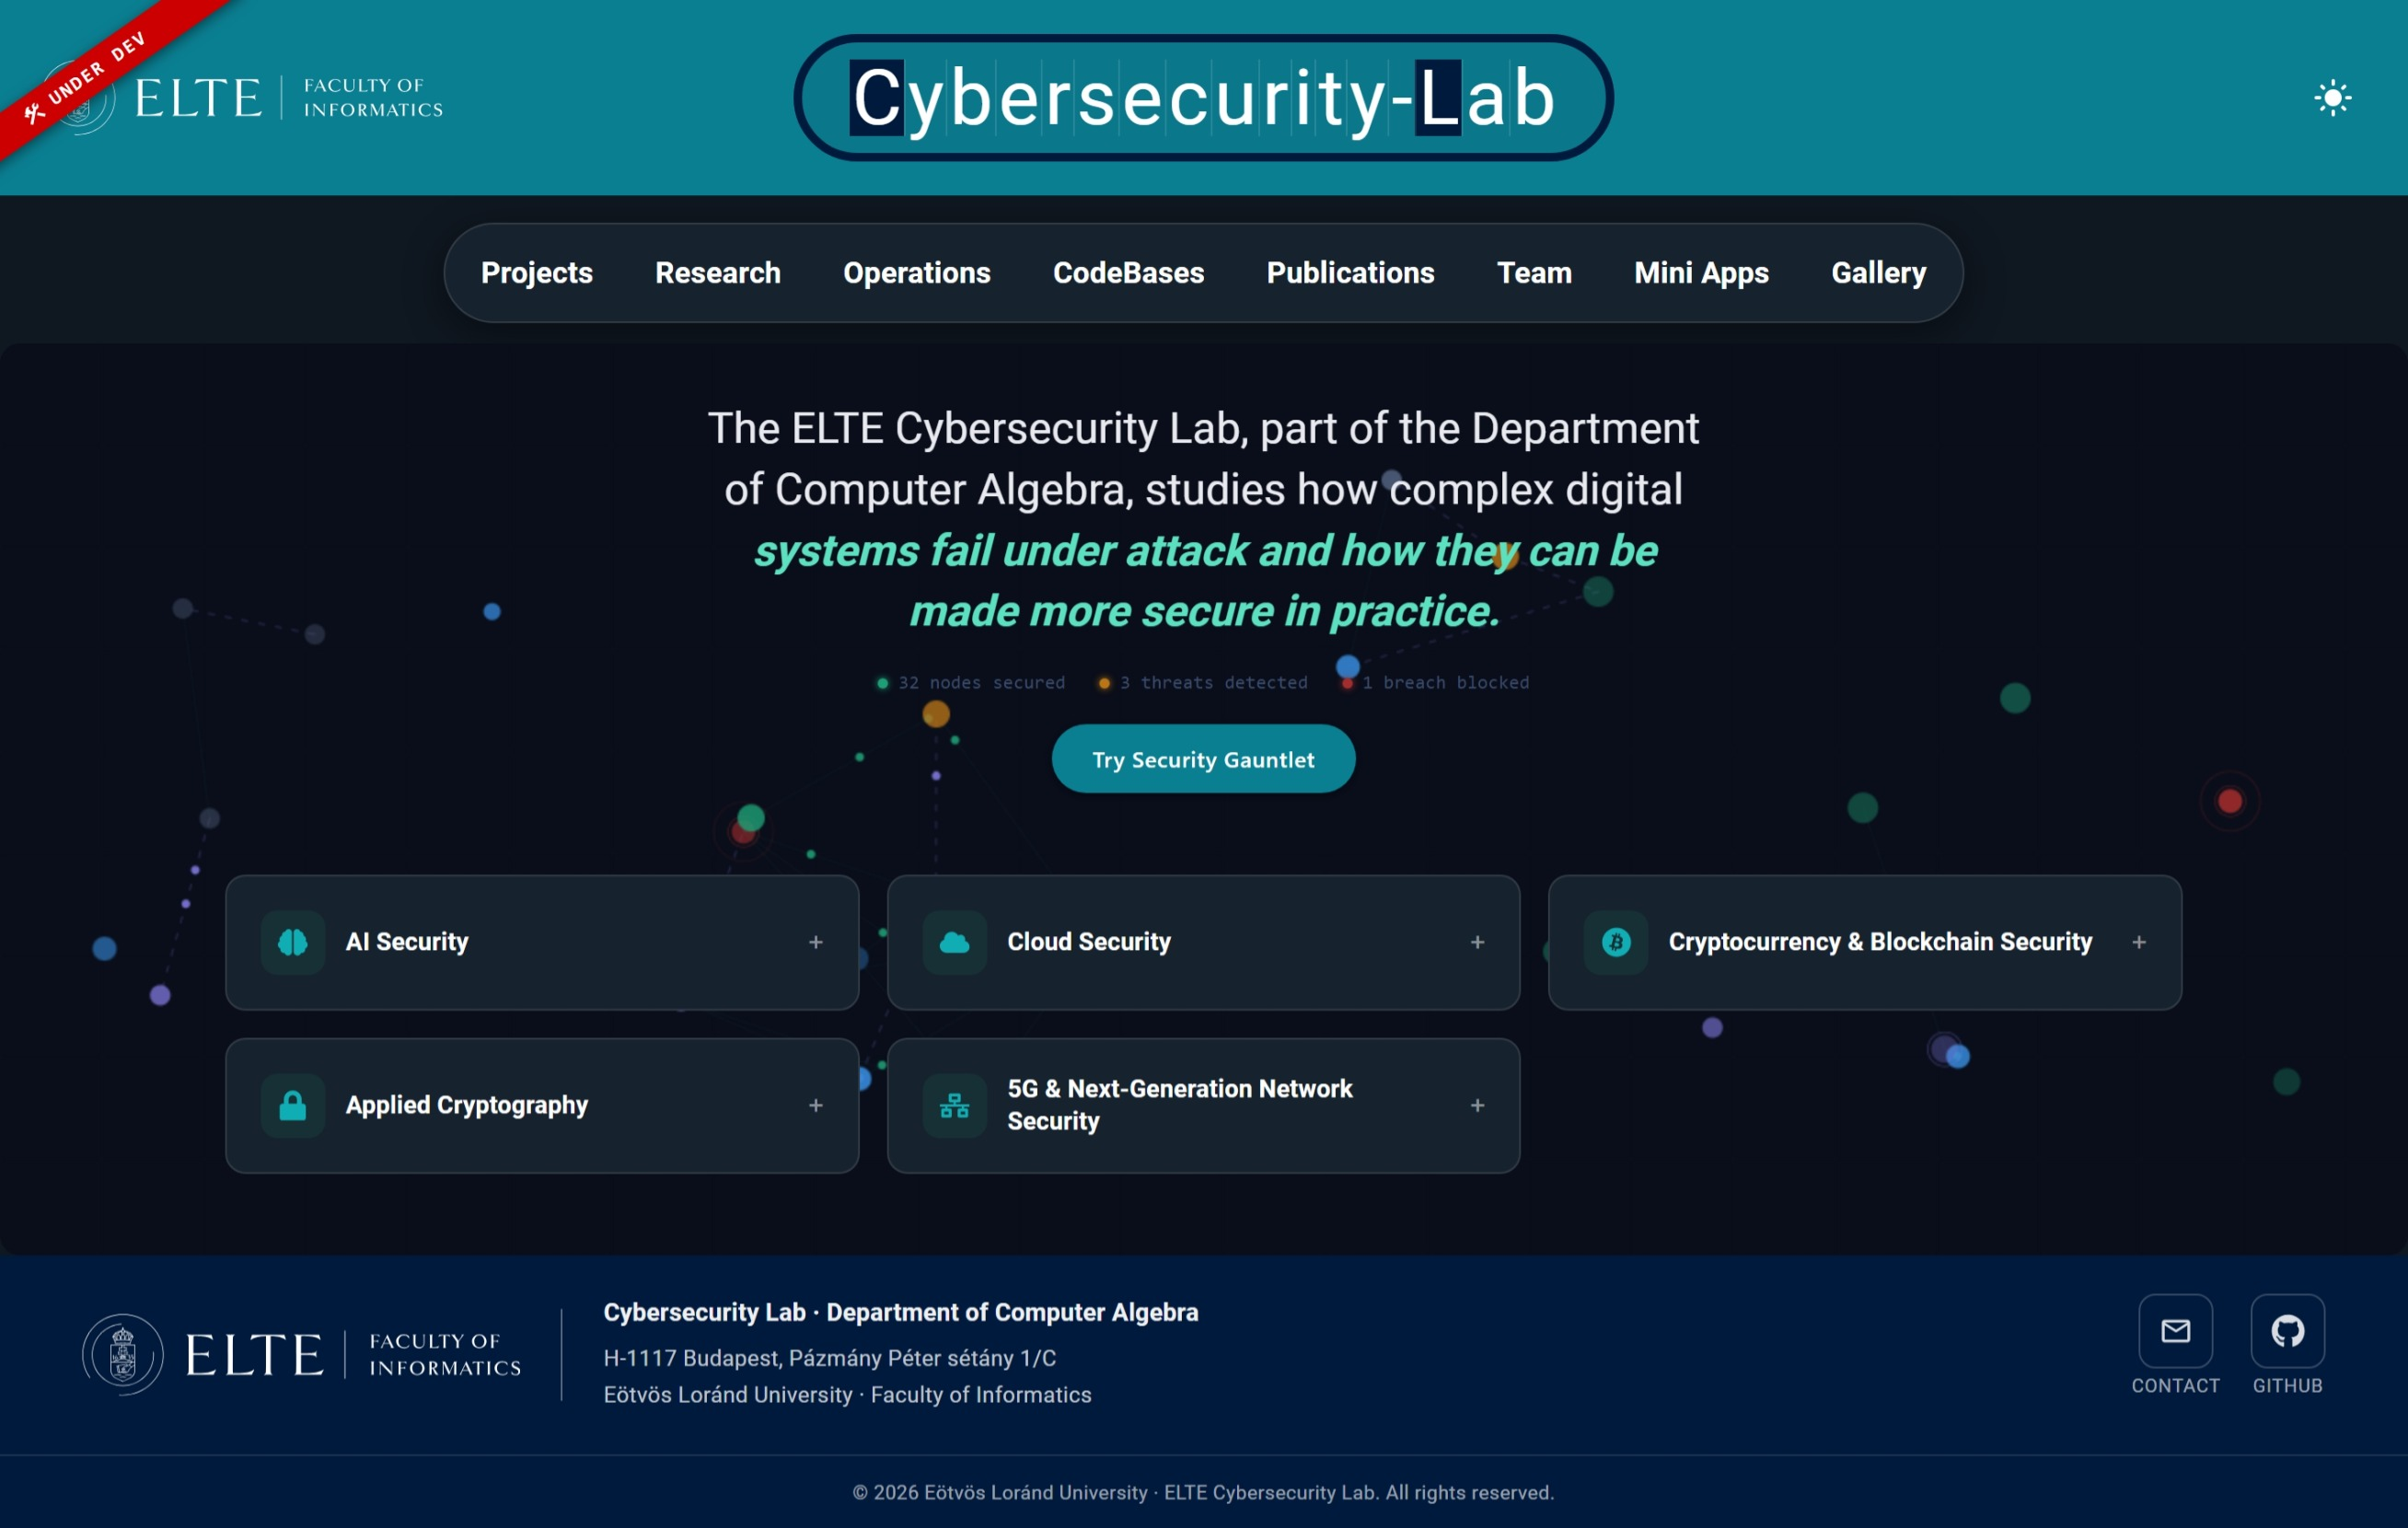
\includegraphics[width=0.88\textwidth]{images/home.jpeg}
	\caption{The Home page with the animated node background, the hexagonal research grid, and the Security Gauntlet card lower down.}
	\label{fig:home}
\end{figure}

\paragraph{Data file.} The text shown on the home page and the list of research areas it displays come from \texttt{src/data/HomePageData.ts}. The file exports \texttt{MainTitle}, a single string used as the lab's headline, and \texttt{researchAreas}, an array of \texttt{\{title, description\}} objects. Editing \texttt{MainTitle} changes the headline. Adding, removing, or editing entries in \texttt{researchAreas} changes the cards under the headline. The file is intentionally lighter than the Research page's data file because the home page shows a simpler summary.

%-----------------------------------------------------------
\section{Projects Page}\label{sec:user-projects}

The Projects page shows the lab's main research projects as a diamond-shaped node graph. There are four outer circles, one per project, and one central circle labelled \textbf{Lab Projects}. The outer circles are colour-coded and labelled with their short names (B5G Network Security, Distributed ML Security, Compliance Verification, Cloud Security).

When the page first loads, the first project in the list is already selected. The selected node is highlighted on the graph and its details appear in the panel on the right of the graph on desktop, and below the graph on mobile. Clicking any other node selects it and updates the panel immediately. The selected panel shows the project's status, the number of sub-projects it has, the number of related projects, a list of keywords, and the names of related projects with which it shares concerns.

Below the graph is the project detail section. It shows the currently selected project's full description, its main objectives (as a bullet list), and its sub-projects. Each sub-project is a collapsible row. Clicking the row expands it to show the sub-project's full description, its focus areas, and any related codebases. Related codebases are shown as clickable links that lead directly to the corresponding CodeBases page entry, so the visitor can move from a project description to the code that supports it without going through the navigation bar.

The number cards at the top of the page (Main Projects, Sub-Projects, Connections) are computed automatically from the data file. They are not edited separately.

\begin{figure}[H]
	\centering
	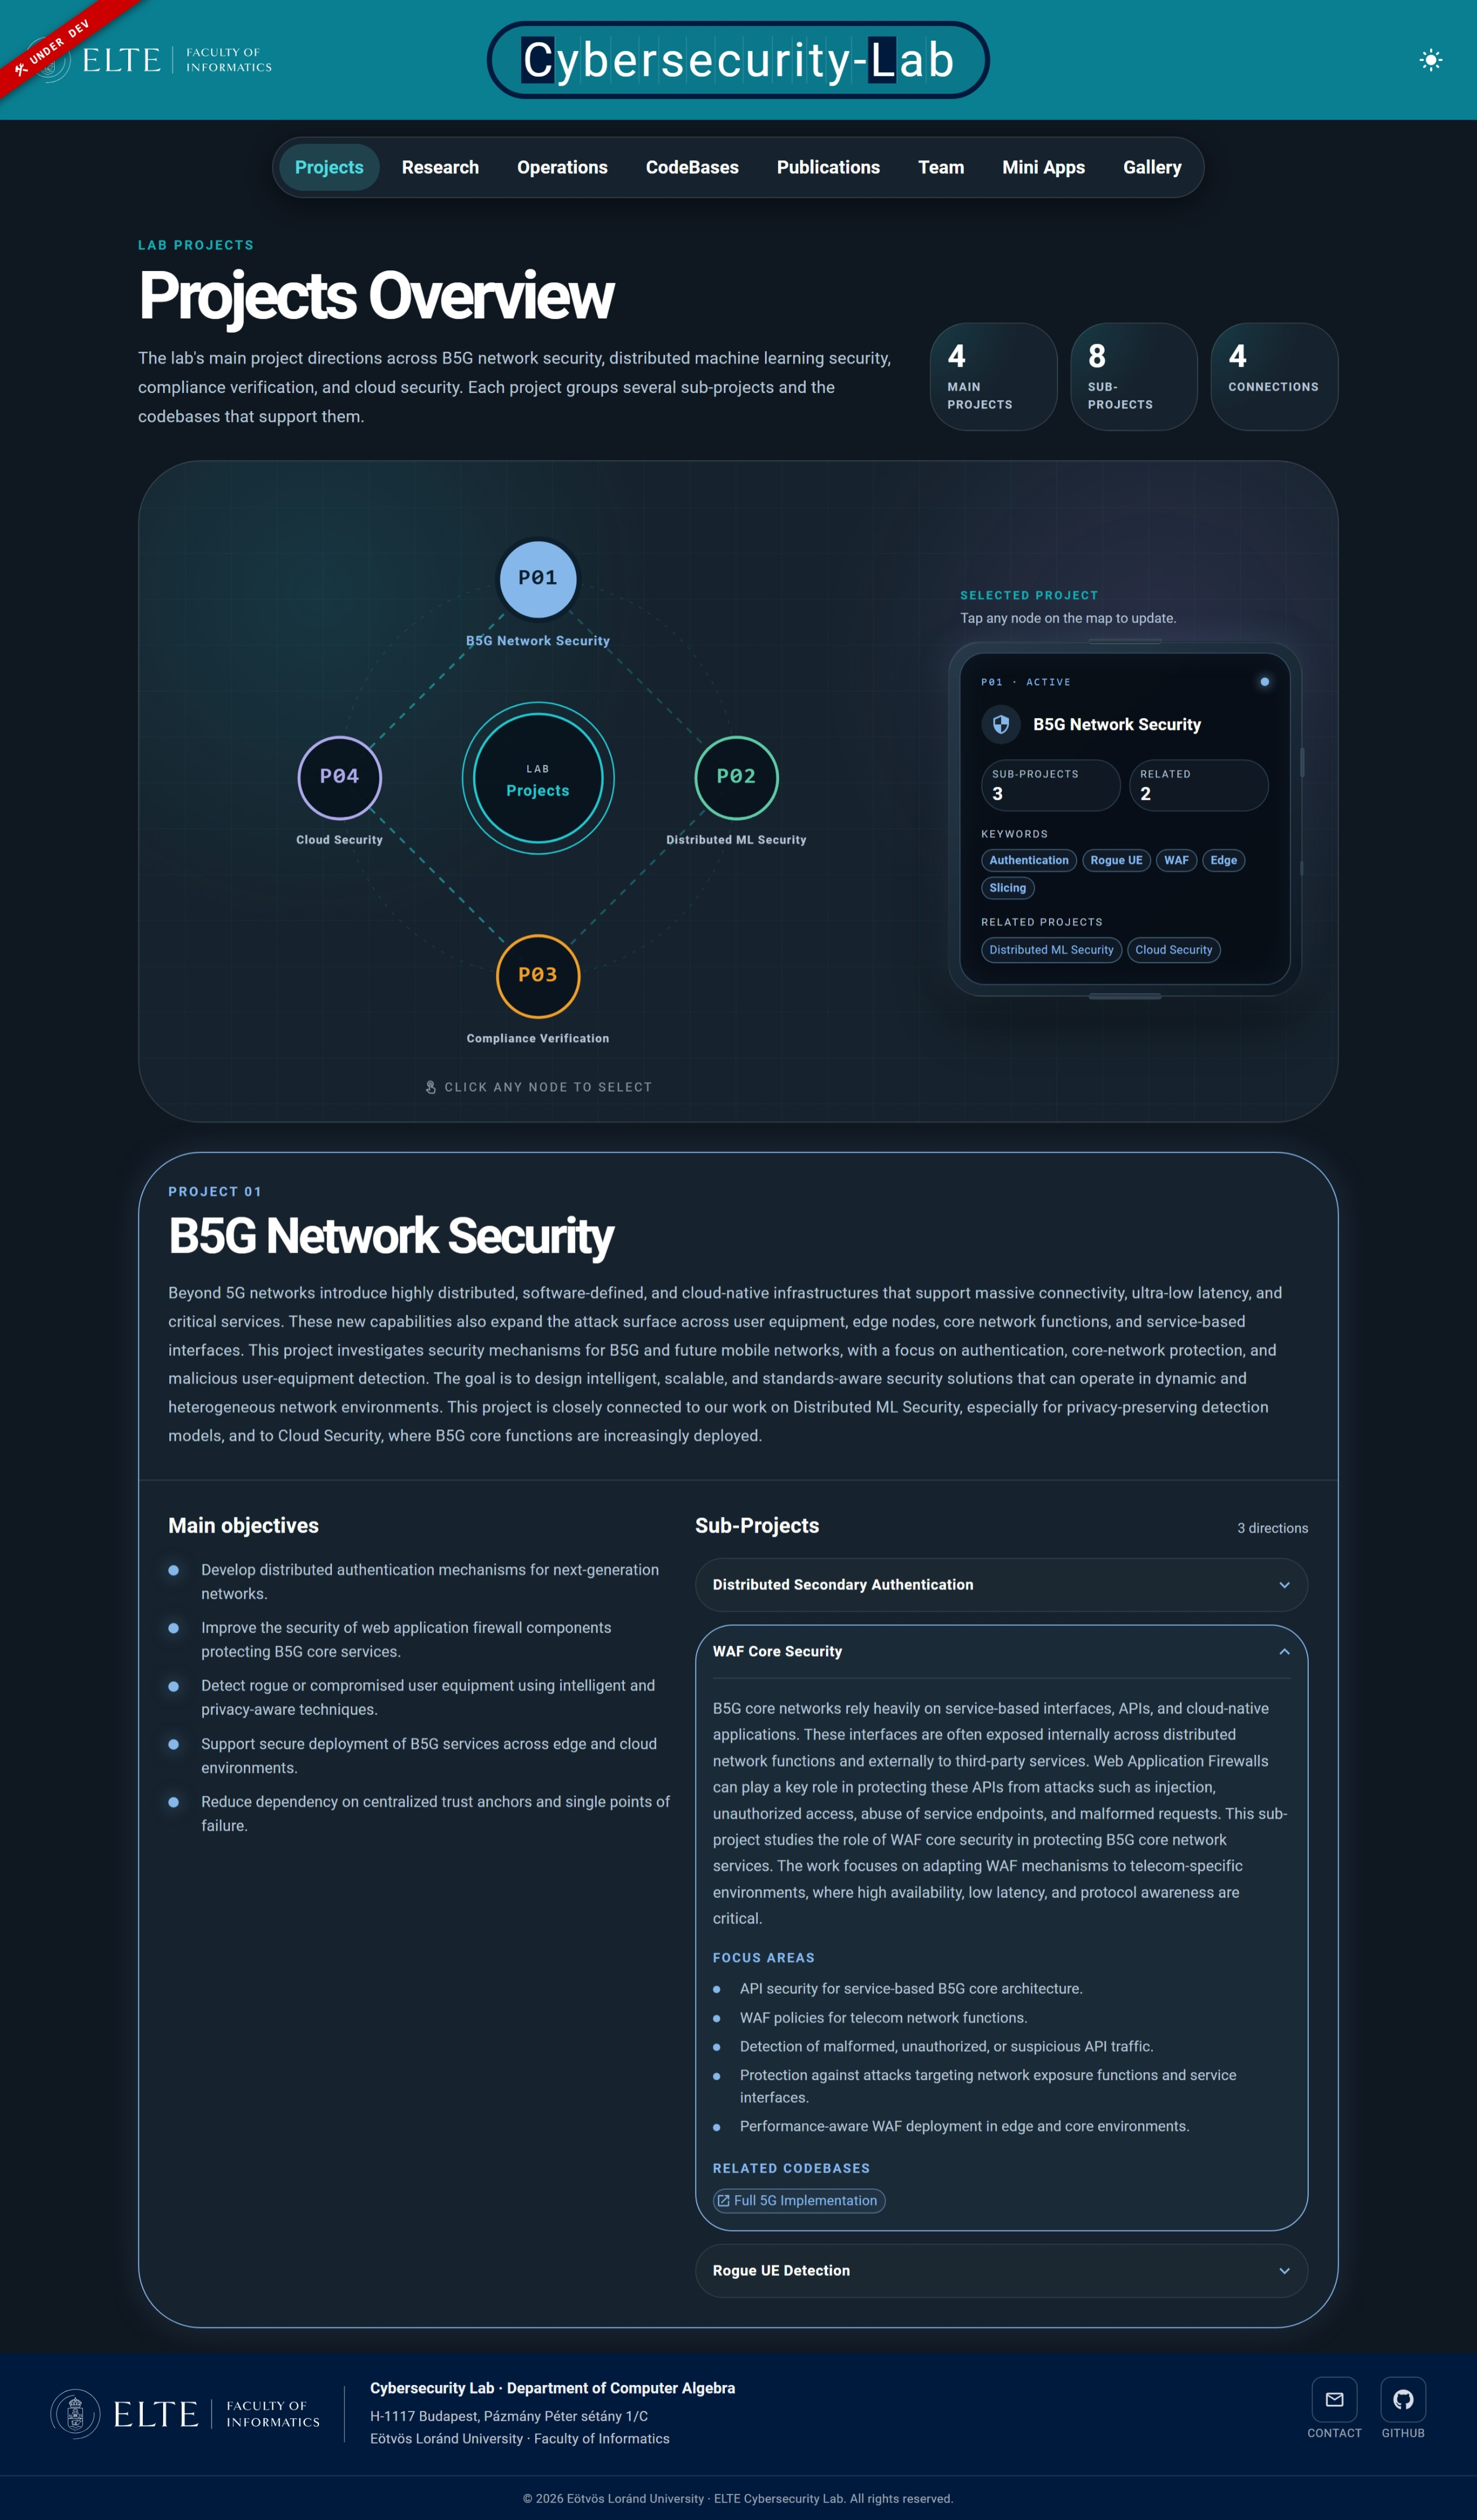
\includegraphics[width=0.72\textwidth]{images/projects.jpeg}
	\caption{The Projects page with the diamond-shaped node graph and the detail panel for the first project (B5G Network Security) open below the graph.}
	\label{fig:projects-page}
\end{figure}

\paragraph{Data file.} The Projects page is driven entirely by \texttt{src/data/projectsPageData.ts}. The file exports an object containing a \texttt{projects} array, where each project entry has a \texttt{slug}, \texttt{title}, \texttt{description}, \texttt{mainObjectives} (a list of strings), \texttt{relatedProjects} (a list of project titles), and \texttt{subProjects} (a list of sub-project objects). Each sub-project has a \texttt{title}, \texttt{description}, \texttt{researchFocus} (a list of strings), and \texttt{codebases} (a list of strings matching codebase slugs).

The \texttt{codebases} field on a sub-project is what creates the link from a project to a CodeBases entry. The portal looks up each string in the list against the codebases data and renders a clickable link if a match is found. The match is by slug, so the string in the project file must correspond to the codebase's identifier; a typo here means the link will not appear, but the rest of the project still renders. The \texttt{relatedProjects} field works similarly: it matches against other project titles in the same file.

%-----------------------------------------------------------
\section{Research Page}\label{sec:user-research}

The Research page presents the lab's research areas as a honeycomb of hexagonal cells. There are six outer cells, one per area, arranged around a central decorative cell that shows a stylised chipset motif. Unlike the Projects page, no area is selected when the page first loads. The visitor has to click a hex to open the detail panel below the honeycomb.

Each hex is coloured according to the area's accent colour, has an icon in its centre (a glyph or a small symbol), and has the area's title underneath. The first load animates the hexes into position around the central chipset on a staggered timer, so the honeycomb assembles itself rather than appearing all at once. Long titles such as \textit{Cryptocurrency and Blockchain Security} are wrapped across multiple lines automatically so they fit inside the hex.

Clicking a hex opens a panel below the honeycomb. The panel shows the area's title, a one-sentence intro in italic, and a longer description. The area's accent colour is used for the panel's heading and side border, which links the hex visually to the panel content. Clicking a different hex updates the panel immediately and re-highlights the selected hex on the honeycomb.

\begin{figure}[H]
	\centering
	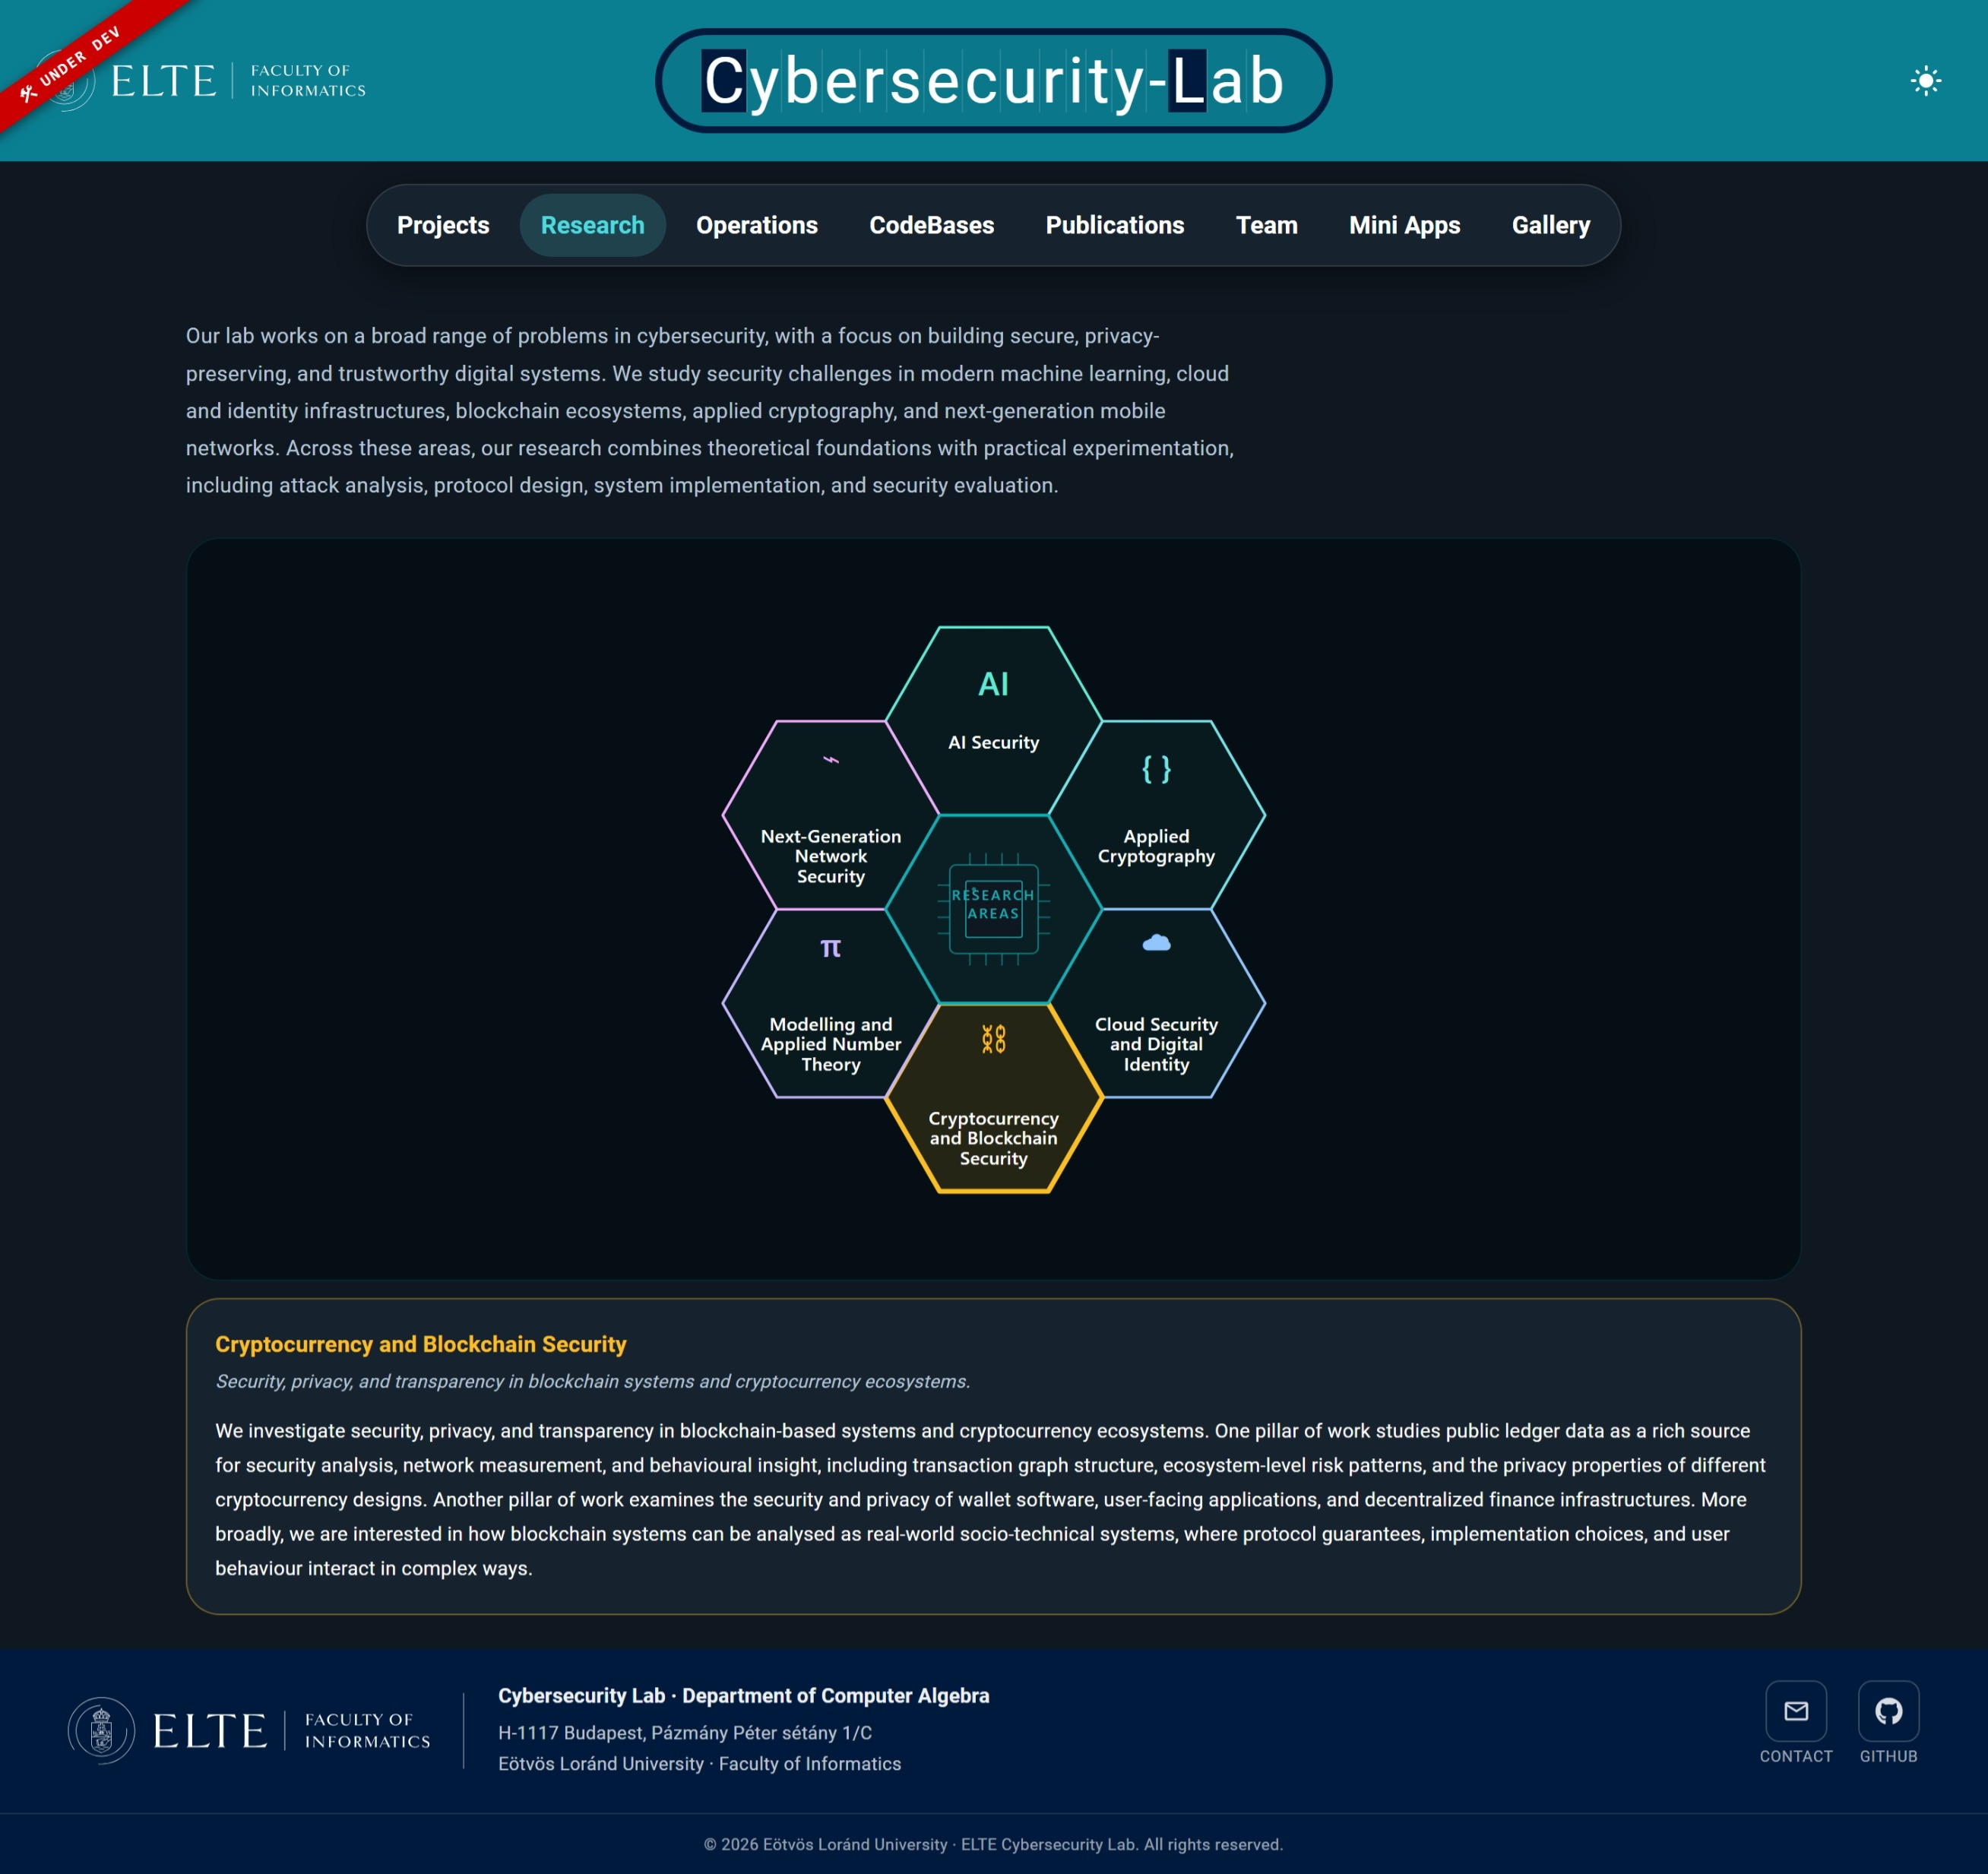
\includegraphics[width=0.88\textwidth]{images/research.jpeg}
	\caption{The Research page with the six-hex honeycomb around the central chipset motif. The Cryptocurrency and Blockchain Security hex is selected and its detail panel is open below the honeycomb.}
	\label{fig:research-page}
\end{figure}

\paragraph{Data file.} The Research page reads from \texttt{src/data/ResearchPageData.ts}. The file exports \texttt{researchPageIntro} (the paragraph shown above the honeycomb) and \texttt{researchAreas} (the array of hex entries). Each research area has an \texttt{id}, \texttt{title}, \texttt{icon}, \texttt{color}, \texttt{intro}, and \texttt{description} field.

The \texttt{color} field accepts any valid CSS colour string and is used for the hex border, the panel heading, and the panel side border. The \texttt{icon} field is a short text glyph rendered inside the hex; using a single character or a couple of characters works best because hexes have limited internal space. Adding a new area requires only a new entry in this array, the honeycomb layout adapts to the number of cells.

%-----------------------------------------------------------
\section{Operations Page}\label{sec:user-operations}

The Operations page describes how the lab organises its work. It opens with a paragraph explaining that lab work is done in small group projects rather than individual assignments. Below the paragraph is the project structure section.

The project structure is shown as a two-by-two grid. The horizontal axis is labelled \textbf{Theory} versus \textbf{Practice}. The vertical axis is labelled \textbf{Builds} versus \textbf{Breaks / Measures}. Each of the four project roles sits in its natural quadrant: \textbf{Theorist} (builds, theory), \textbf{Engineer} (builds, practice), \textbf{Attacker} (breaks, theory), and \textbf{Evaluator} (breaks, practice). The axis labels are rendered with rotated text using CSS transforms so that they sit alongside their corresponding axes.

Each quadrant is clickable, in the same interaction style as the Research honeycomb. Clicking a quadrant opens a detail panel to the right of the grid on desktop and below it on mobile. The panel shows the role's full description and uses the role's colour as an accent. Like the honeycomb, the quadrants animate into place on first load on a staggered timer.

Below the grid is a section on the lab's guiding principles. Three principles are listed: \textbf{Supervision}, \textbf{Open Source}, and \textbf{Teamwork as Training}. Each principle has a short text on one side and an interactive visual component on the other. The visual components are small custom illustrations that respond to the visitor:

\begin{itemize}
	\item \textbf{Supervision} uses an eye whose pupil tracks the visitor's mouse cursor across the page. The eye is meant to suggest the continuous attention a supervisor gives to a student project.
	\item \textbf{Open Source} uses a central code-symbol node with several coloured satellite dots that drift outward when the visitor's cursor enters the component. It is meant to suggest the way open-source contributions spread to the broader community.
	\item \textbf{Teamwork as Training} uses a cluster of small hexagons that connect to each other with lines when the visitor hovers the component. It is meant to suggest individual contributions integrating into a single coherent result.
\end{itemize}

Each visual is purely decorative; nothing important is hidden inside the interaction. On small screens the visual column is hidden and the prose takes the full width so that the principles stay readable on mobile.

\begin{figure}[H]
	\centering
	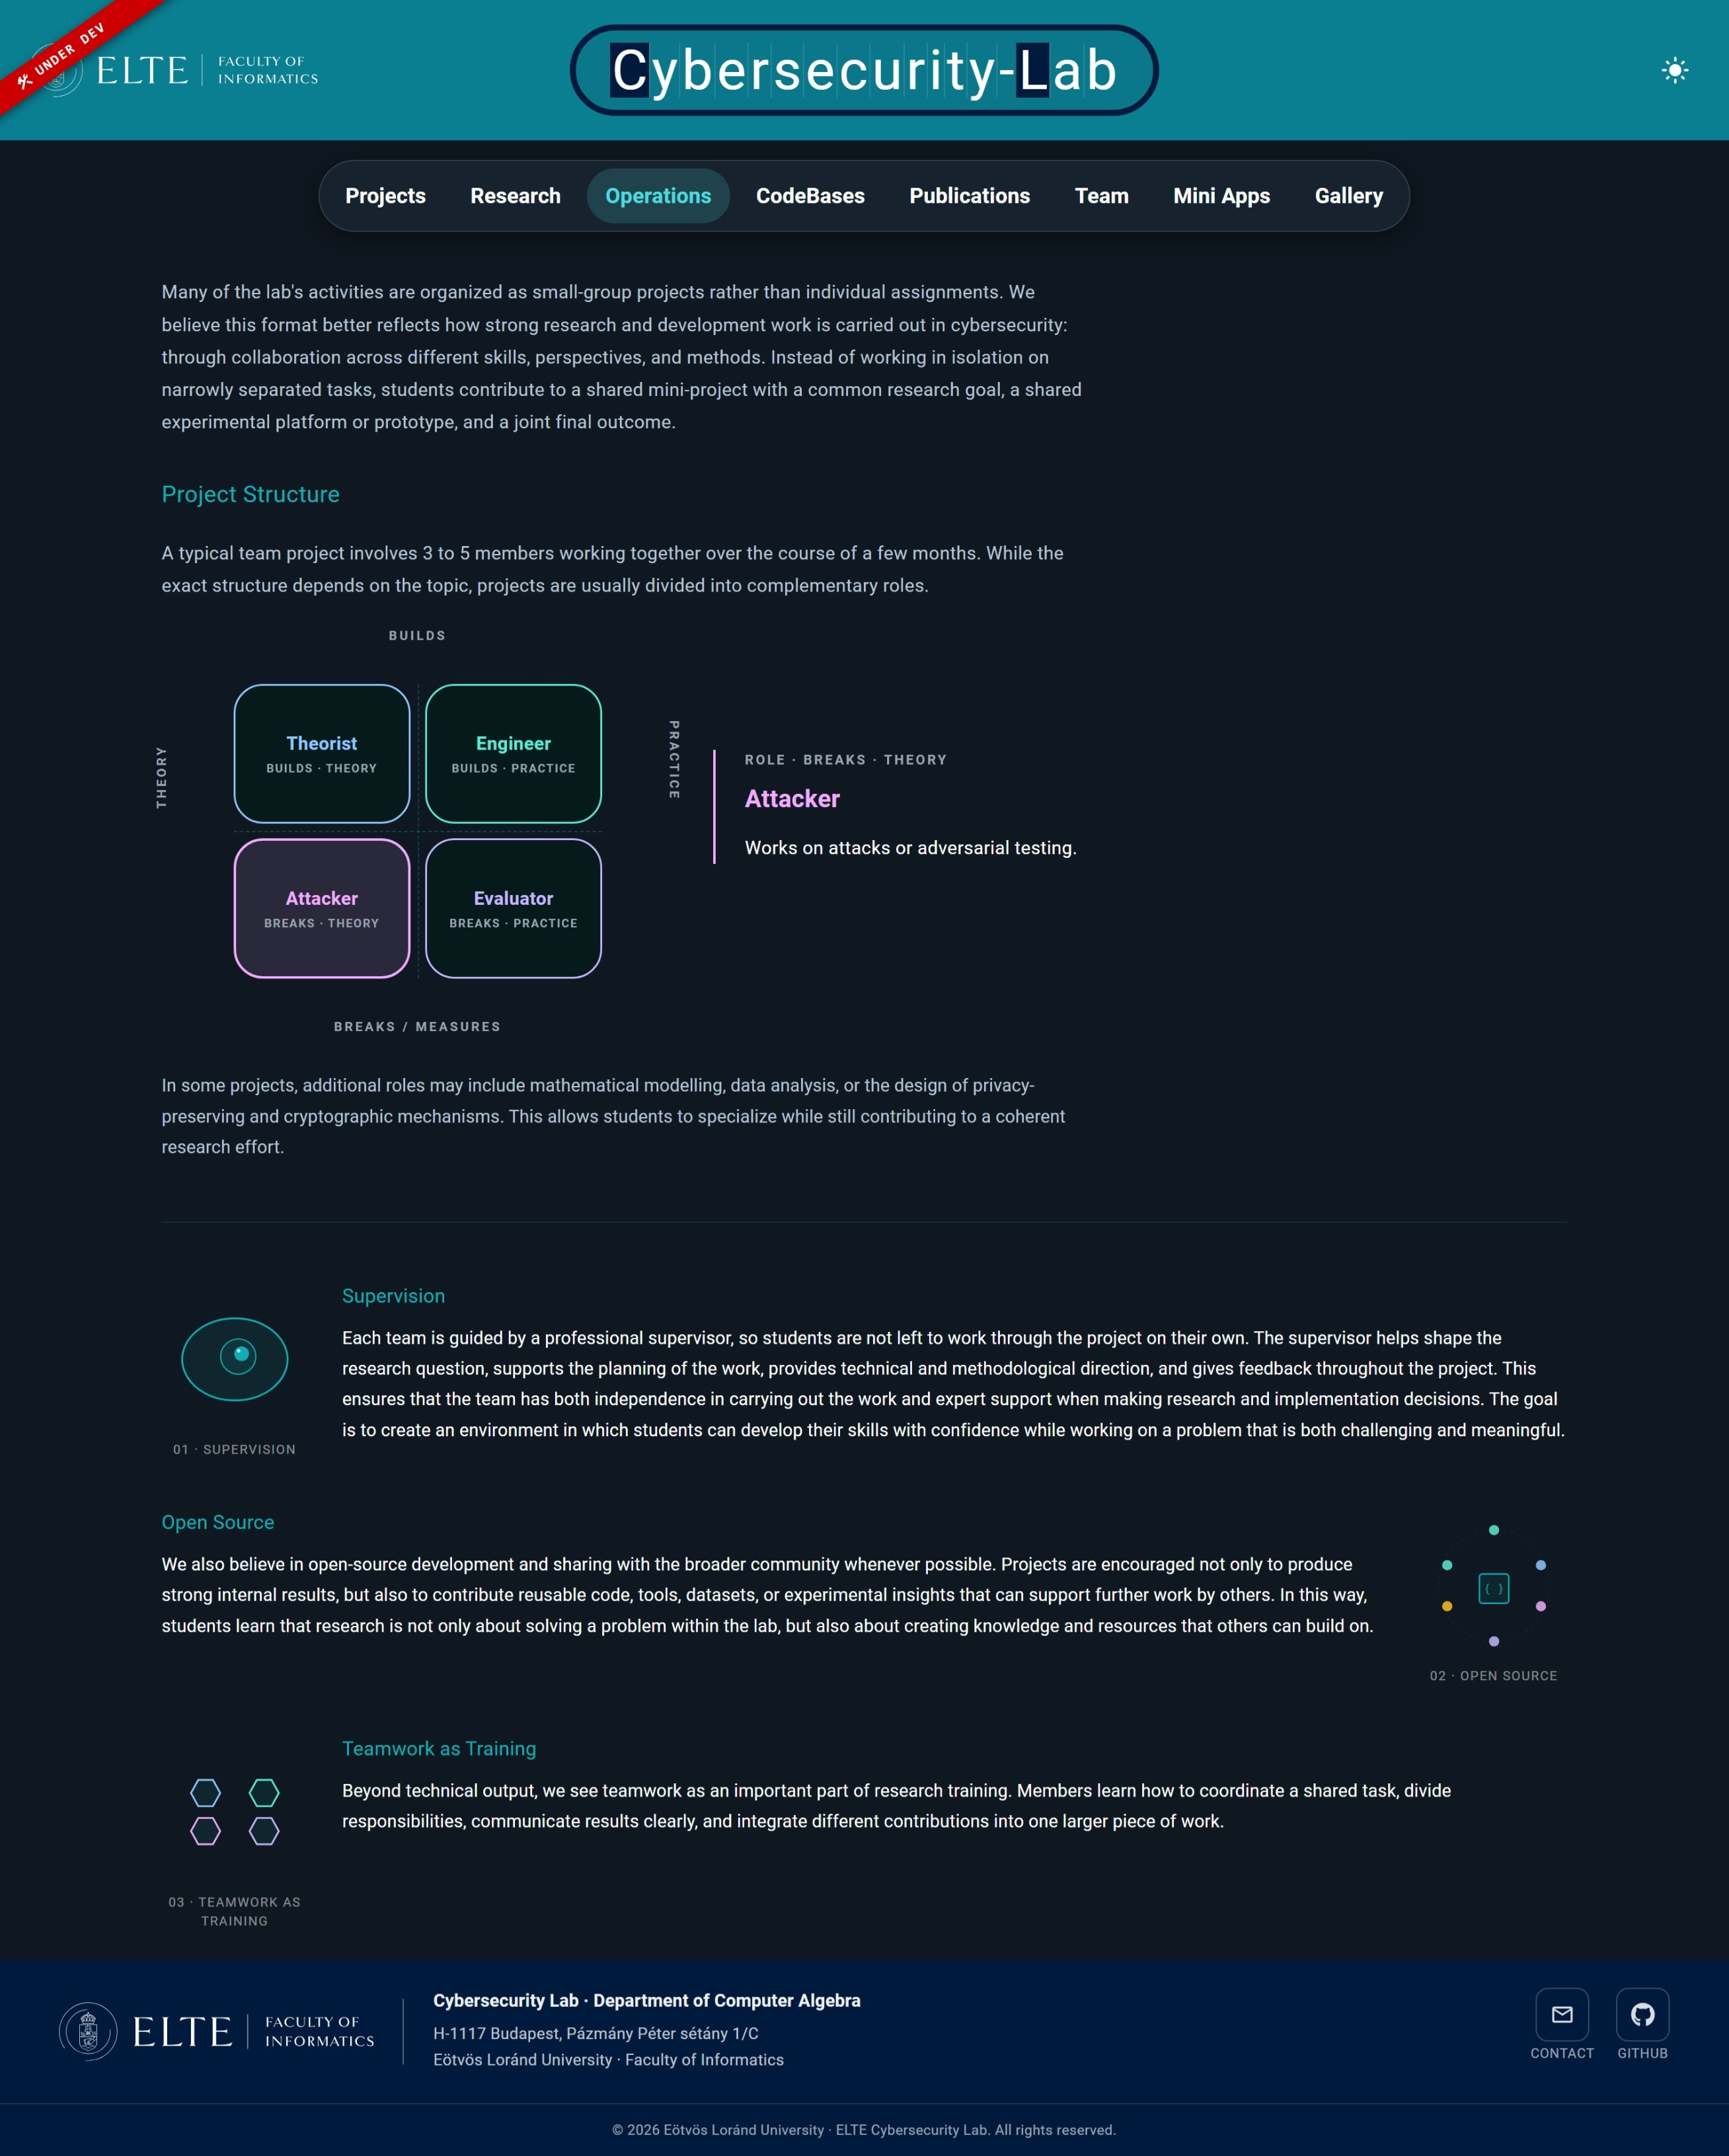
\includegraphics[width=0.88\textwidth]{images/operations.jpeg}
	\caption{The Operations page with the two-by-two role grid (the Attacker quadrant selected and showing its description on the right), and the three principles with their interactive visual components below.}
	\label{fig:operations-page}
\end{figure}

\paragraph{Data file.} The Operations page reads from \texttt{src/data/operationPageData.ts}. The file exports a single \texttt{operationPageData} object containing the intro paragraph, the structure heading and intro, the four roles (each with an \texttt{id}, \texttt{role}, \texttt{description}, axis assignment, and colours for both light and dark mode), the additional roles paragraph, and the three principles.

Each principle entry has an \texttt{id}, \texttt{title}, \texttt{description}, an optional \texttt{componentKey}, and an optional \texttt{iconFallback}. The \texttt{componentKey} field is what binds a principle to its interactive visual. The page keeps a small registry mapping component keys (\texttt{mentorEye}, \texttt{shareOrbit}, \texttt{teamPulse}) to the actual React components that render the visuals. When the page renders a principle, it looks up the \texttt{componentKey} in the registry; if the key is found, the corresponding visual is rendered, and if it is not found, the \texttt{iconFallback} value is used to render a Material UI icon instead. This means adding a new principle whose visual already exists in the registry requires no code changes at all; only a new entry in the data file. Adding a new visual requires adding one component file and one line in the registry, after which it is available to all data entries.

%-----------------------------------------------------------
\section{CodeBases Page}\label{sec:user-codebases}

The CodeBases page is the page the project was built around. It shows the lab's public repositories as a grid of cards, each card representing one repository. Each card shows the repository's logo (or a default icon if the repository does not have one), the repository's title, a short description, and two actions: \textbf{View repository} (which opens the GitHub page in a new tab) and \textbf{Open Project} (which opens the structured walkthrough for that repository).

Above the grid is a sort control with options for sorting by newest first, oldest first, title ascending, or title descending. The cards reorder on the page when the sort option is changed.

\begin{figure}[H]
	\centering
	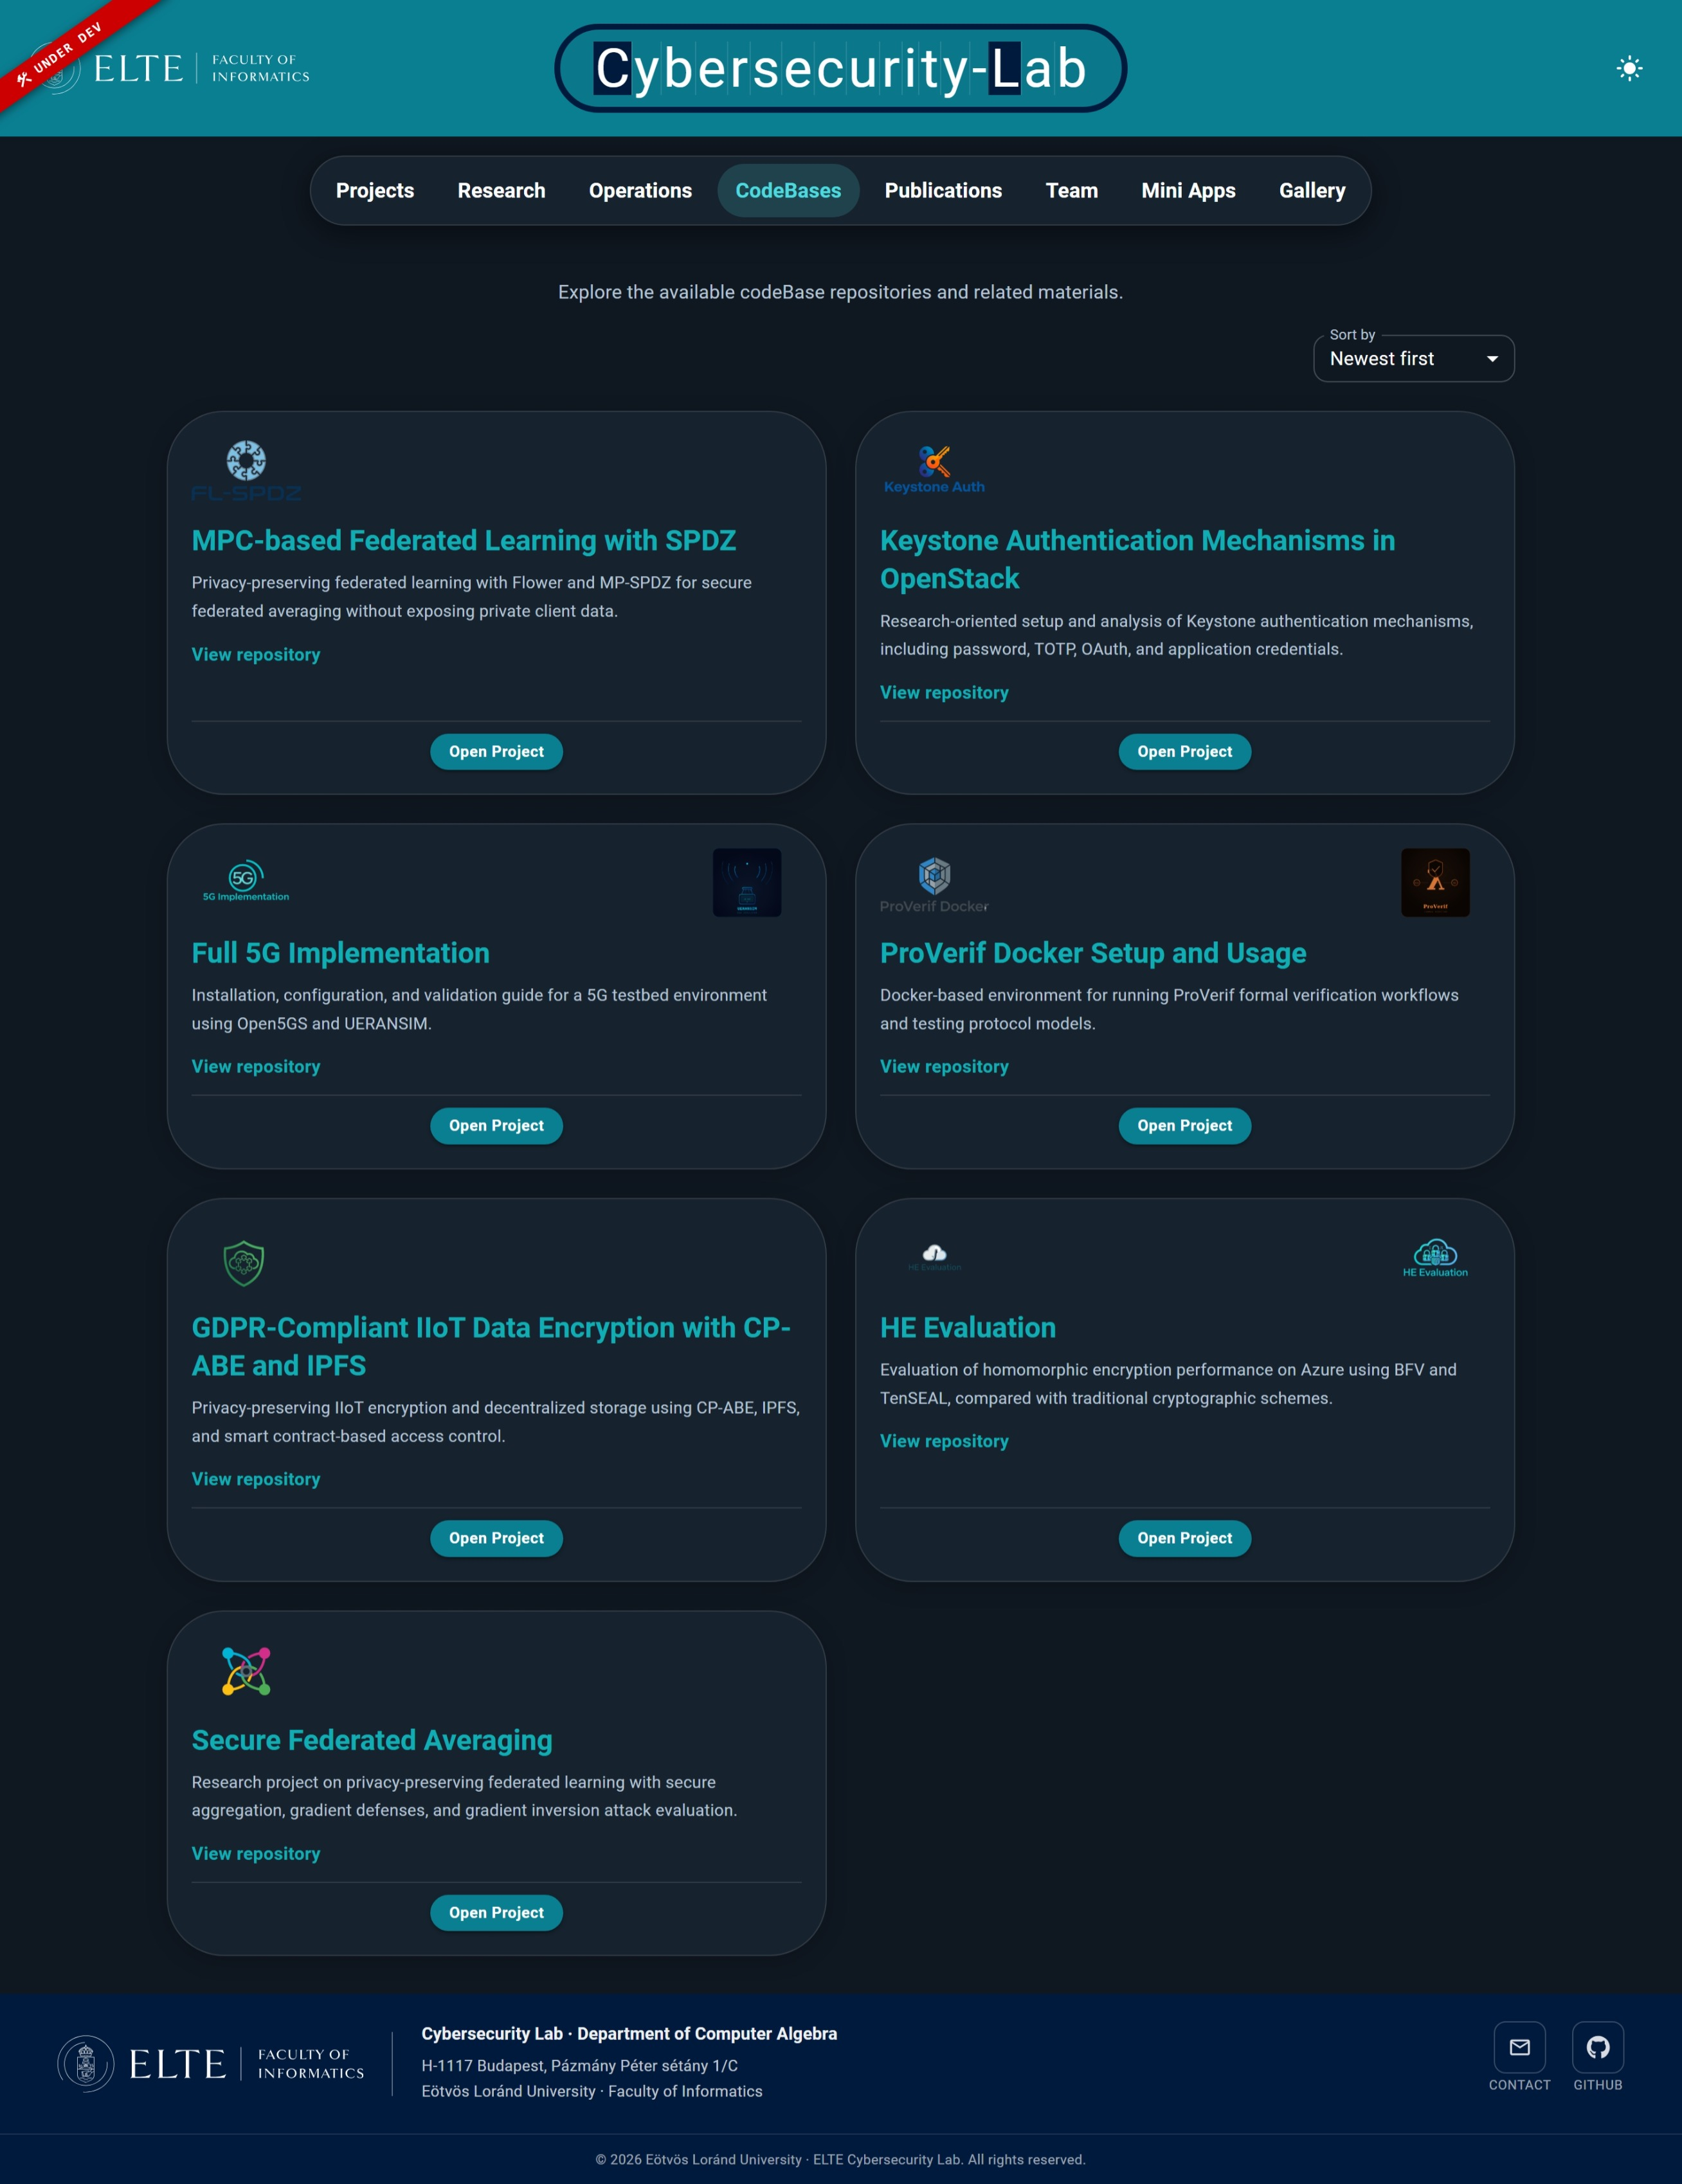
\includegraphics[width=0.88\textwidth]{images/codebases.jpeg}
	\caption{The CodeBases page with the grid of repository cards, each showing the project logo, title, short description, and two actions (View repository, Open Project).}
	\label{fig:codebases-page}
\end{figure}

Clicking \textbf{Open Project} loads a structured documentation view for the repository. On the left side of this view is a sidebar listing the topics of the documentation: \textbf{Overview}, \textbf{System Requirements}, \textbf{Hardware Setup}, \textbf{Software Installation}, \textbf{Build Instructions}, \textbf{Machines Overview}, \textbf{Configuration}, \textbf{Validation \& Testing}, \textbf{Troubleshooting}, and \textbf{References}. The exact list of topics depends on the repository; the sidebar is built from the structure of the Markdown document, not from a fixed list.

Clicking a topic in the sidebar loads only that topic into the main panel. The visitor reads one section at a time, in the same way they would read one chapter of a course at a time. At the bottom of each section there are \textbf{Back} and \textbf{Next} buttons that move to the previous and next topic in the sidebar. The current topic is highlighted in the sidebar and the highlight follows the visitor as they move through the documentation.

The content of each topic is rendered with full Markdown support: code blocks, tables, headings, links, lists, and images all render the way they would on GitHub. The lab's brand colour and dark theme are applied to the rendered content so the documentation looks like part of the portal rather than an embedded GitHub page.

\begin{figure}[H]
	\centering
	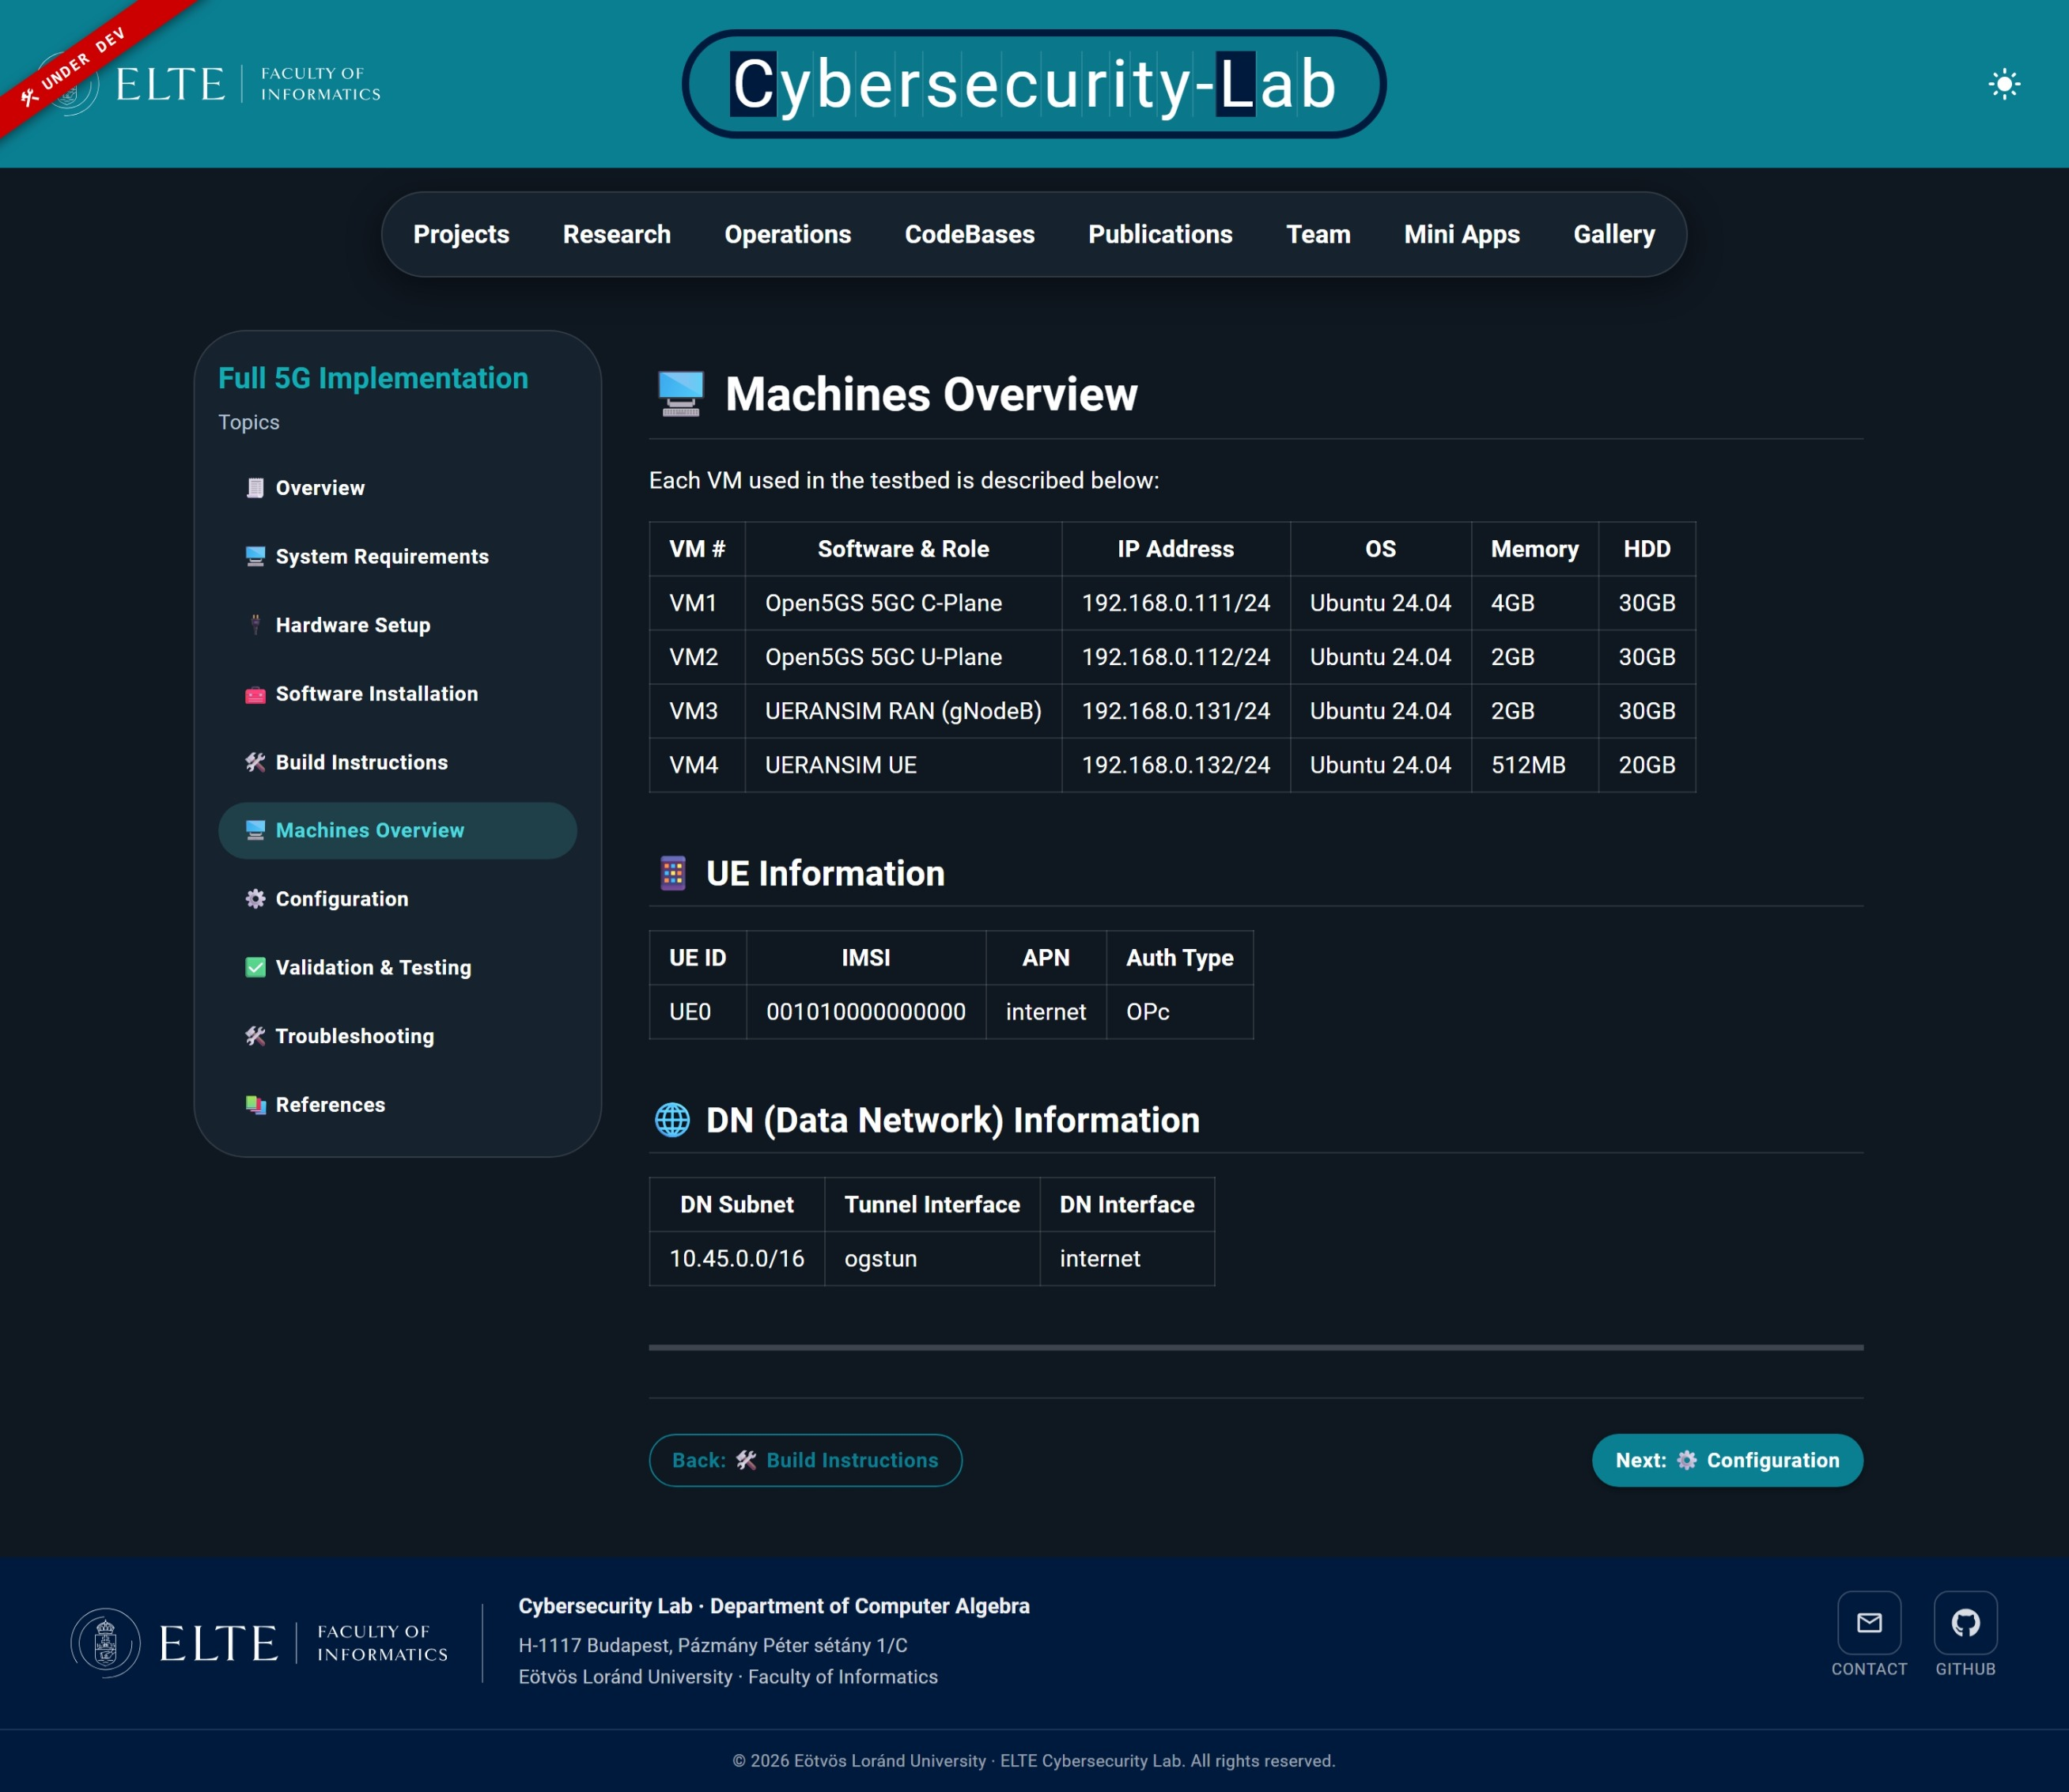
\includegraphics[width=0.88\textwidth]{images/codebase-sample.jpeg}
	\caption{A repository's detail view, showing the topic sidebar on the left and the rendered content of the selected topic (Machines Overview) on the right, with Back and Next buttons at the bottom.}
	\label{fig:codebases-detail}
\end{figure}

\paragraph{How the topics are decided.} The topics are taken directly from the Markdown file for the repository. The portal parses the file and uses the second-level Markdown headings (\texttt{\#\#}) as the top-level topics in the sidebar. Third-level headings (\texttt{\#\#\#}) become sub-topics inside a topic. The first-level heading (\texttt{\#}) is the repository's title. This is what makes the chapter-like feel work: the repository owner controls the structure of their own documentation by structuring the Markdown correctly, and the portal renders that structure as a navigable course.

\paragraph{Metadata block.} Each repository's Markdown file includes a small metadata block near the top, written as a \texttt{\#\# PORTAL\_METADATA} heading followed by a \texttt{portal} fenced code block. The block holds fields the portal uses to render the card on the CodeBases page: \texttt{slug}, \texttt{title}, \texttt{summary}, \texttt{startDate}, \texttt{endDate}, \texttt{repositoryUrl}, and a list of \texttt{logos}. The parser reads this block before walking the rest of the document and uses its values for the card and the routing. If the block is missing, the portal falls back to the file slug and a generic title.

\paragraph{Data file.} The list of repositories on the CodeBases page is built from the Markdown files in \texttt{src/content/}. Each file represents one repository's documentation and is loaded at build time by Vite. The metadata for each card (title, slug, summary, logos, etc.) comes from the metadata block inside each file, so adding a new repository to the portal is a matter of dropping a new \texttt{.md} file into \texttt{src/content/} that follows the agreed heading convention and has a valid metadata block. A template Markdown file is included in the project so anyone setting up a new repository for the lab can copy it and use it as a starting point.

%-----------------------------------------------------------
\section{Publications Page}\label{sec:user-publications}

The Publications page lists the lab's publications as a vertical list of rows. Each row shows the publication's ID, its type tag (\textbf{CONF} for conference, \textbf{JOUR} for journal, \textbf{BOOK} for book chapter), a small venue logo, the publication title, and the publication year. The row is collapsed by default and shows only this summary information.

Above the list is a filter section. There are four type filters at the top (\textbf{All}, \textbf{Conference}, \textbf{Journal}, \textbf{Book Chapter}) and three controls below: a search field that matches publication titles, a year input that filters by year, and an author dropdown populated automatically with the unique author names found in the publications data. Selecting a type filter or filling in any of the search controls narrows the list immediately.

Clicking a publication row expands it. The expanded view shows the authors, the venue with its logo, the abstract, a row of hashtag tags, and an \textbf{Access File} button. Clicking \textbf{Access File} opens the publication's URL in a new tab, where the visitor can find the full text.

The hashtags are clickable. Clicking a hashtag adds it to the active filter set as a removable pill, shown in a row labelled \textbf{ACTIVE} below the search controls. Multiple tags use AND semantics, so each additional tag narrows the list further. When two or more filters are active, a \textbf{Clear All} button appears next to them for one-click reset. Clicking a hashtag also automatically collapses the publication row and scrolls the page back up to the filter section so the visitor sees the new filter being added.

\begin{figure}[H]
	\centering
	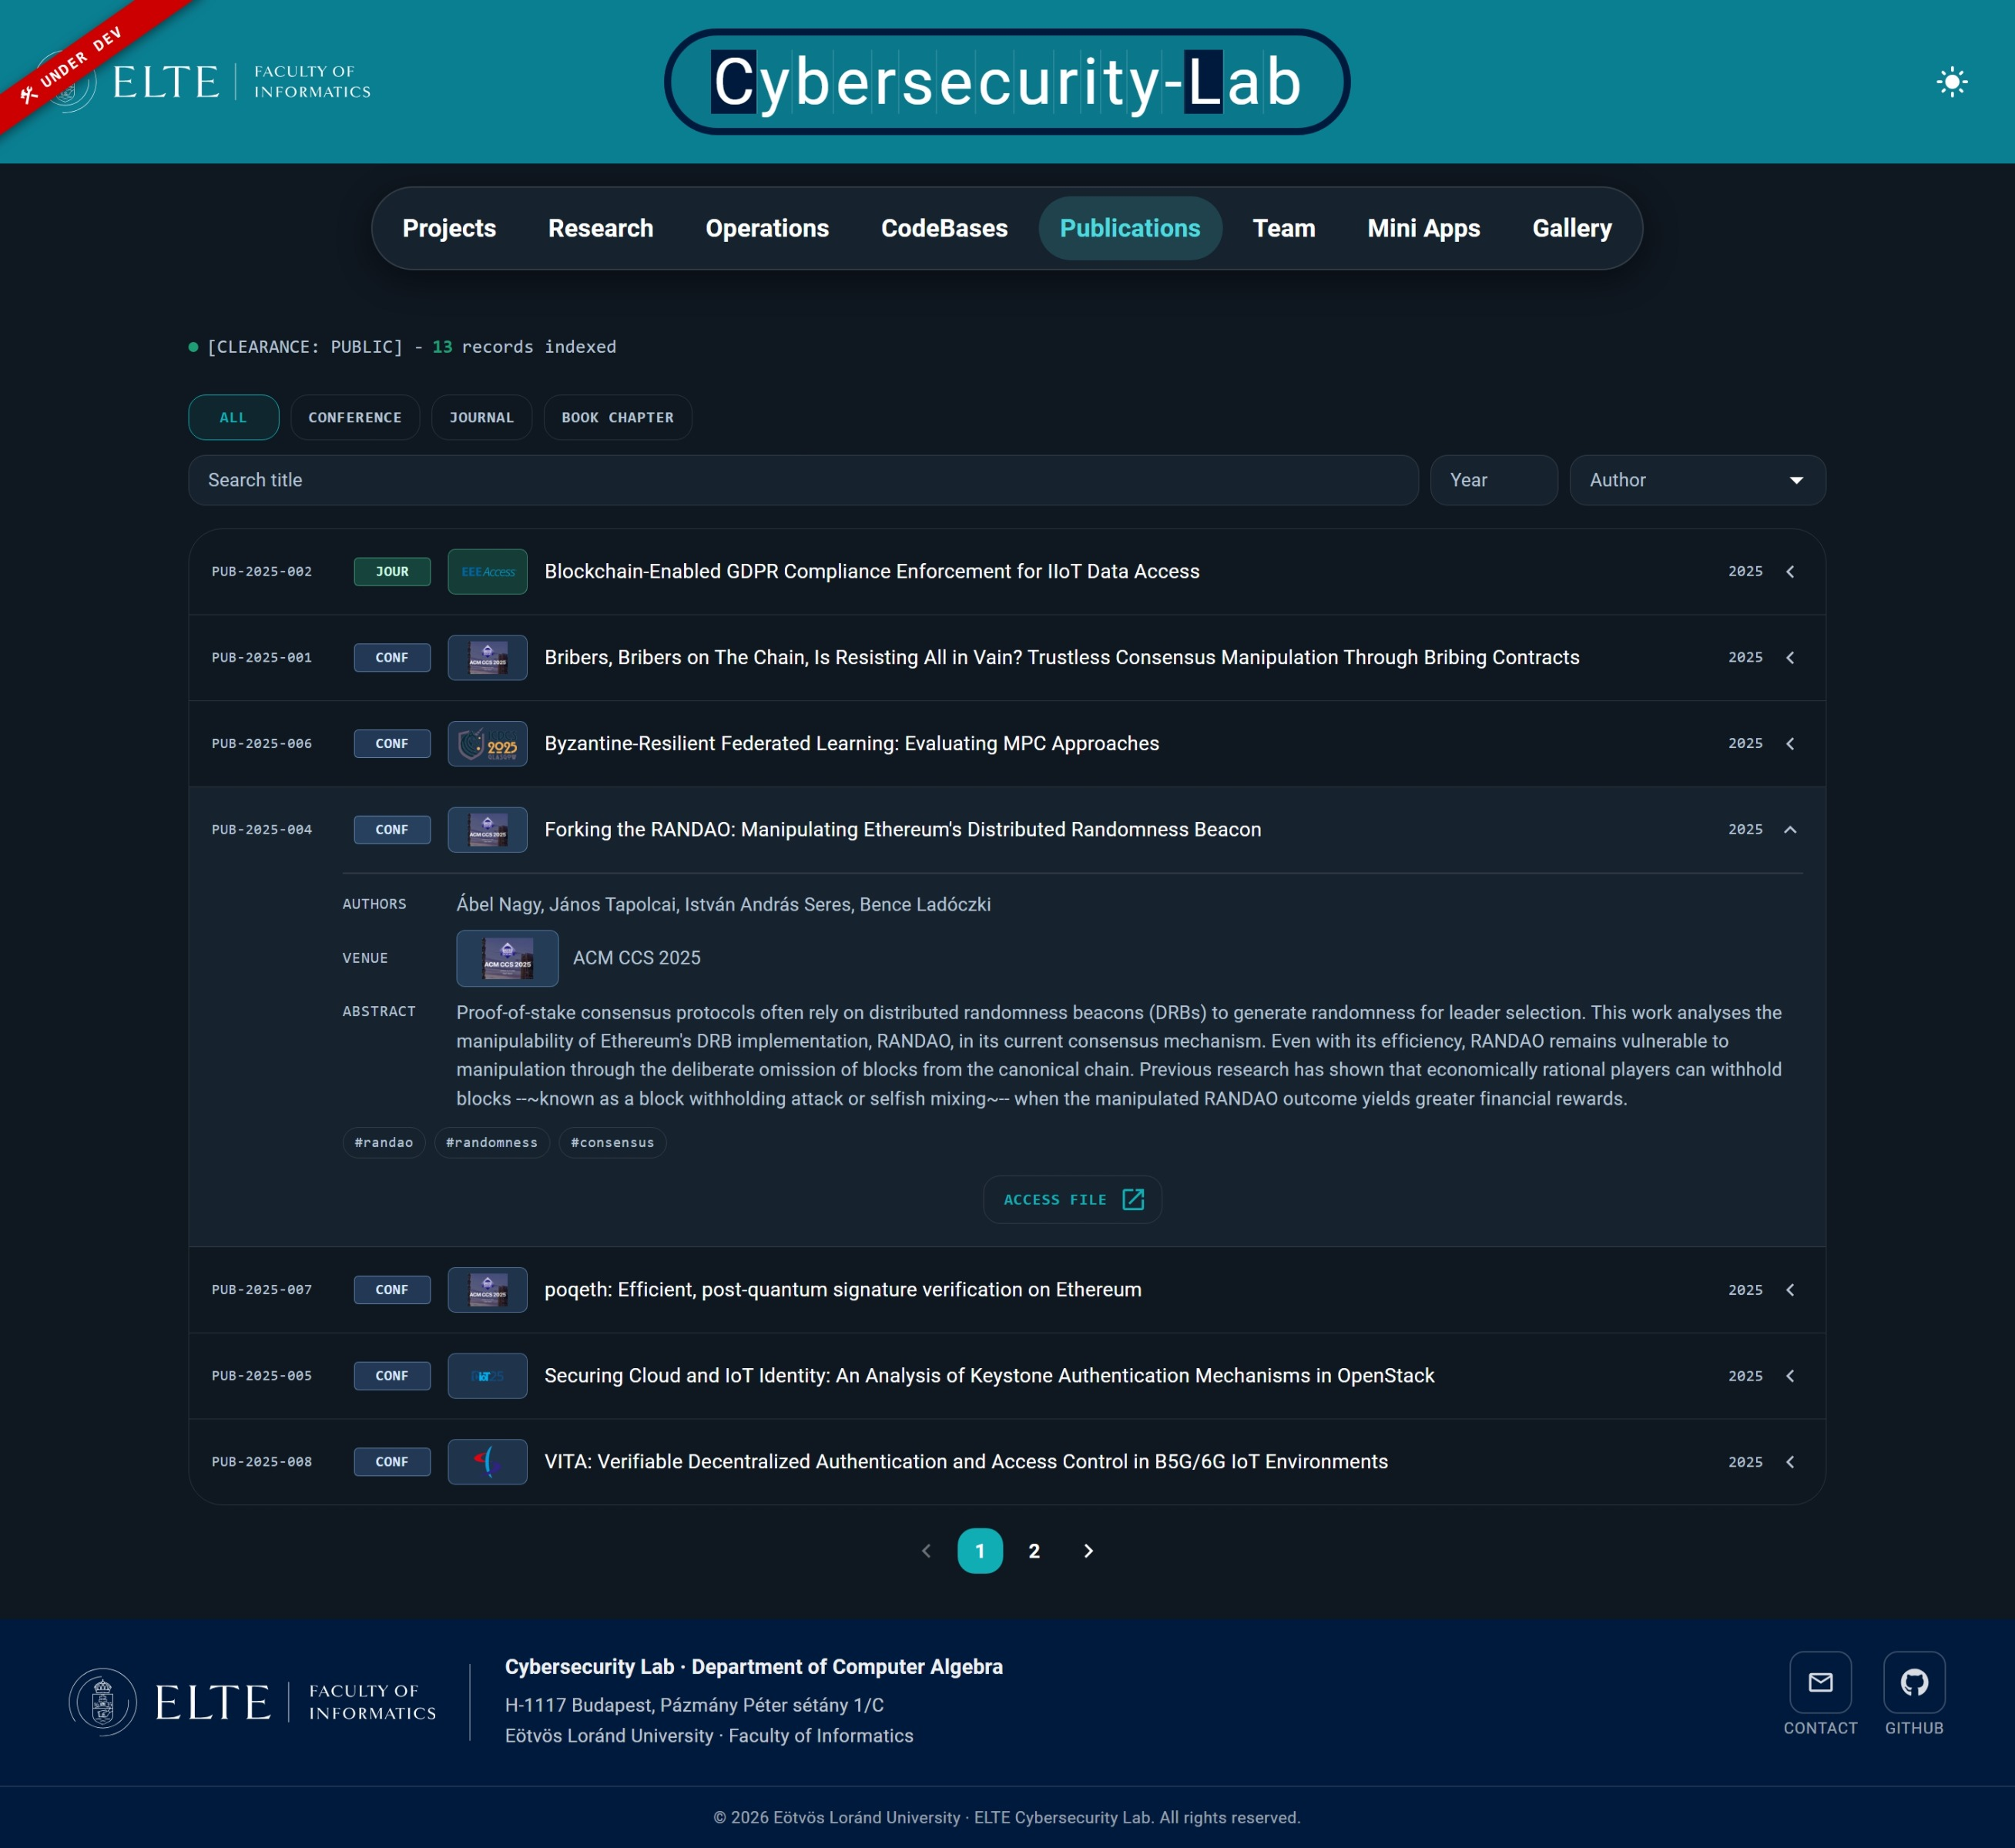
\includegraphics[width=0.88\textwidth]{images/publications_.jpeg}
	\caption{The Publications page with the type filters at the top, the search controls below them, and the publication list. The Forking the RANDAO entry is expanded to show its authors, venue, abstract, hashtags, and Access File button.}
	\label{fig:publications-page}
\end{figure}

\paragraph{Data file.} The Publications page reads from \texttt{src/data/publicationsData.ts}. Each publication entry has a code, a title, an author list, a venue, a year, a type (conference, journal, or book chapter), an abstract, a tag list, a URL pointing to the publication, and a \texttt{venueImage} field for the small logo shown next to the title. Adding a publication is a single new entry in this file. The type filters, the year input, the author dropdown, and the hashtag clicks all work off the same data with no other configuration needed.

%-----------------------------------------------------------
\section{Team Page}\label{sec:user-team}

The Team page introduces the people behind the lab. It is organised as a list of categories, each with its own group of members. The current categories are \textbf{Members} (the lab's faculty and researchers), \textbf{Developer} (the people who built the portal), and \textbf{Students Alumni} (former students of the lab).

Each category has a header row showing the category name, a thin divider, and the number of members in that category. The header is clickable and toggles the category open or closed. By default every category opens on first load.

Inside the \textbf{Members} and \textbf{Developer} categories, each member is shown as a full card: a circular avatar on the left (or a default avatar if no picture is provided), then the member's name (linked to their personal page if a link is set), their role, and a short biographical paragraph.

Inside the \textbf{Students Alumni} category, each member is shown as a smaller card containing just the avatar and the name. On desktop, alumni are paired two per row inside a shared bordered container with a vertical divider between the pair. On mobile, each alumnus is shown as its own card on its own row. The reason for two different layouts is a layout bug that appeared during development: the paired layout used a fixed grid that did not stack cleanly on mobile, and long alumni names like \textit{Arun Chittuparambil Polson} pushed the grid wider than the mobile viewport. The page now switches to single-card mobile layout below a certain breakpoint and the page no longer scrolls horizontally on small screens.

\begin{figure}[H]
	\centering
	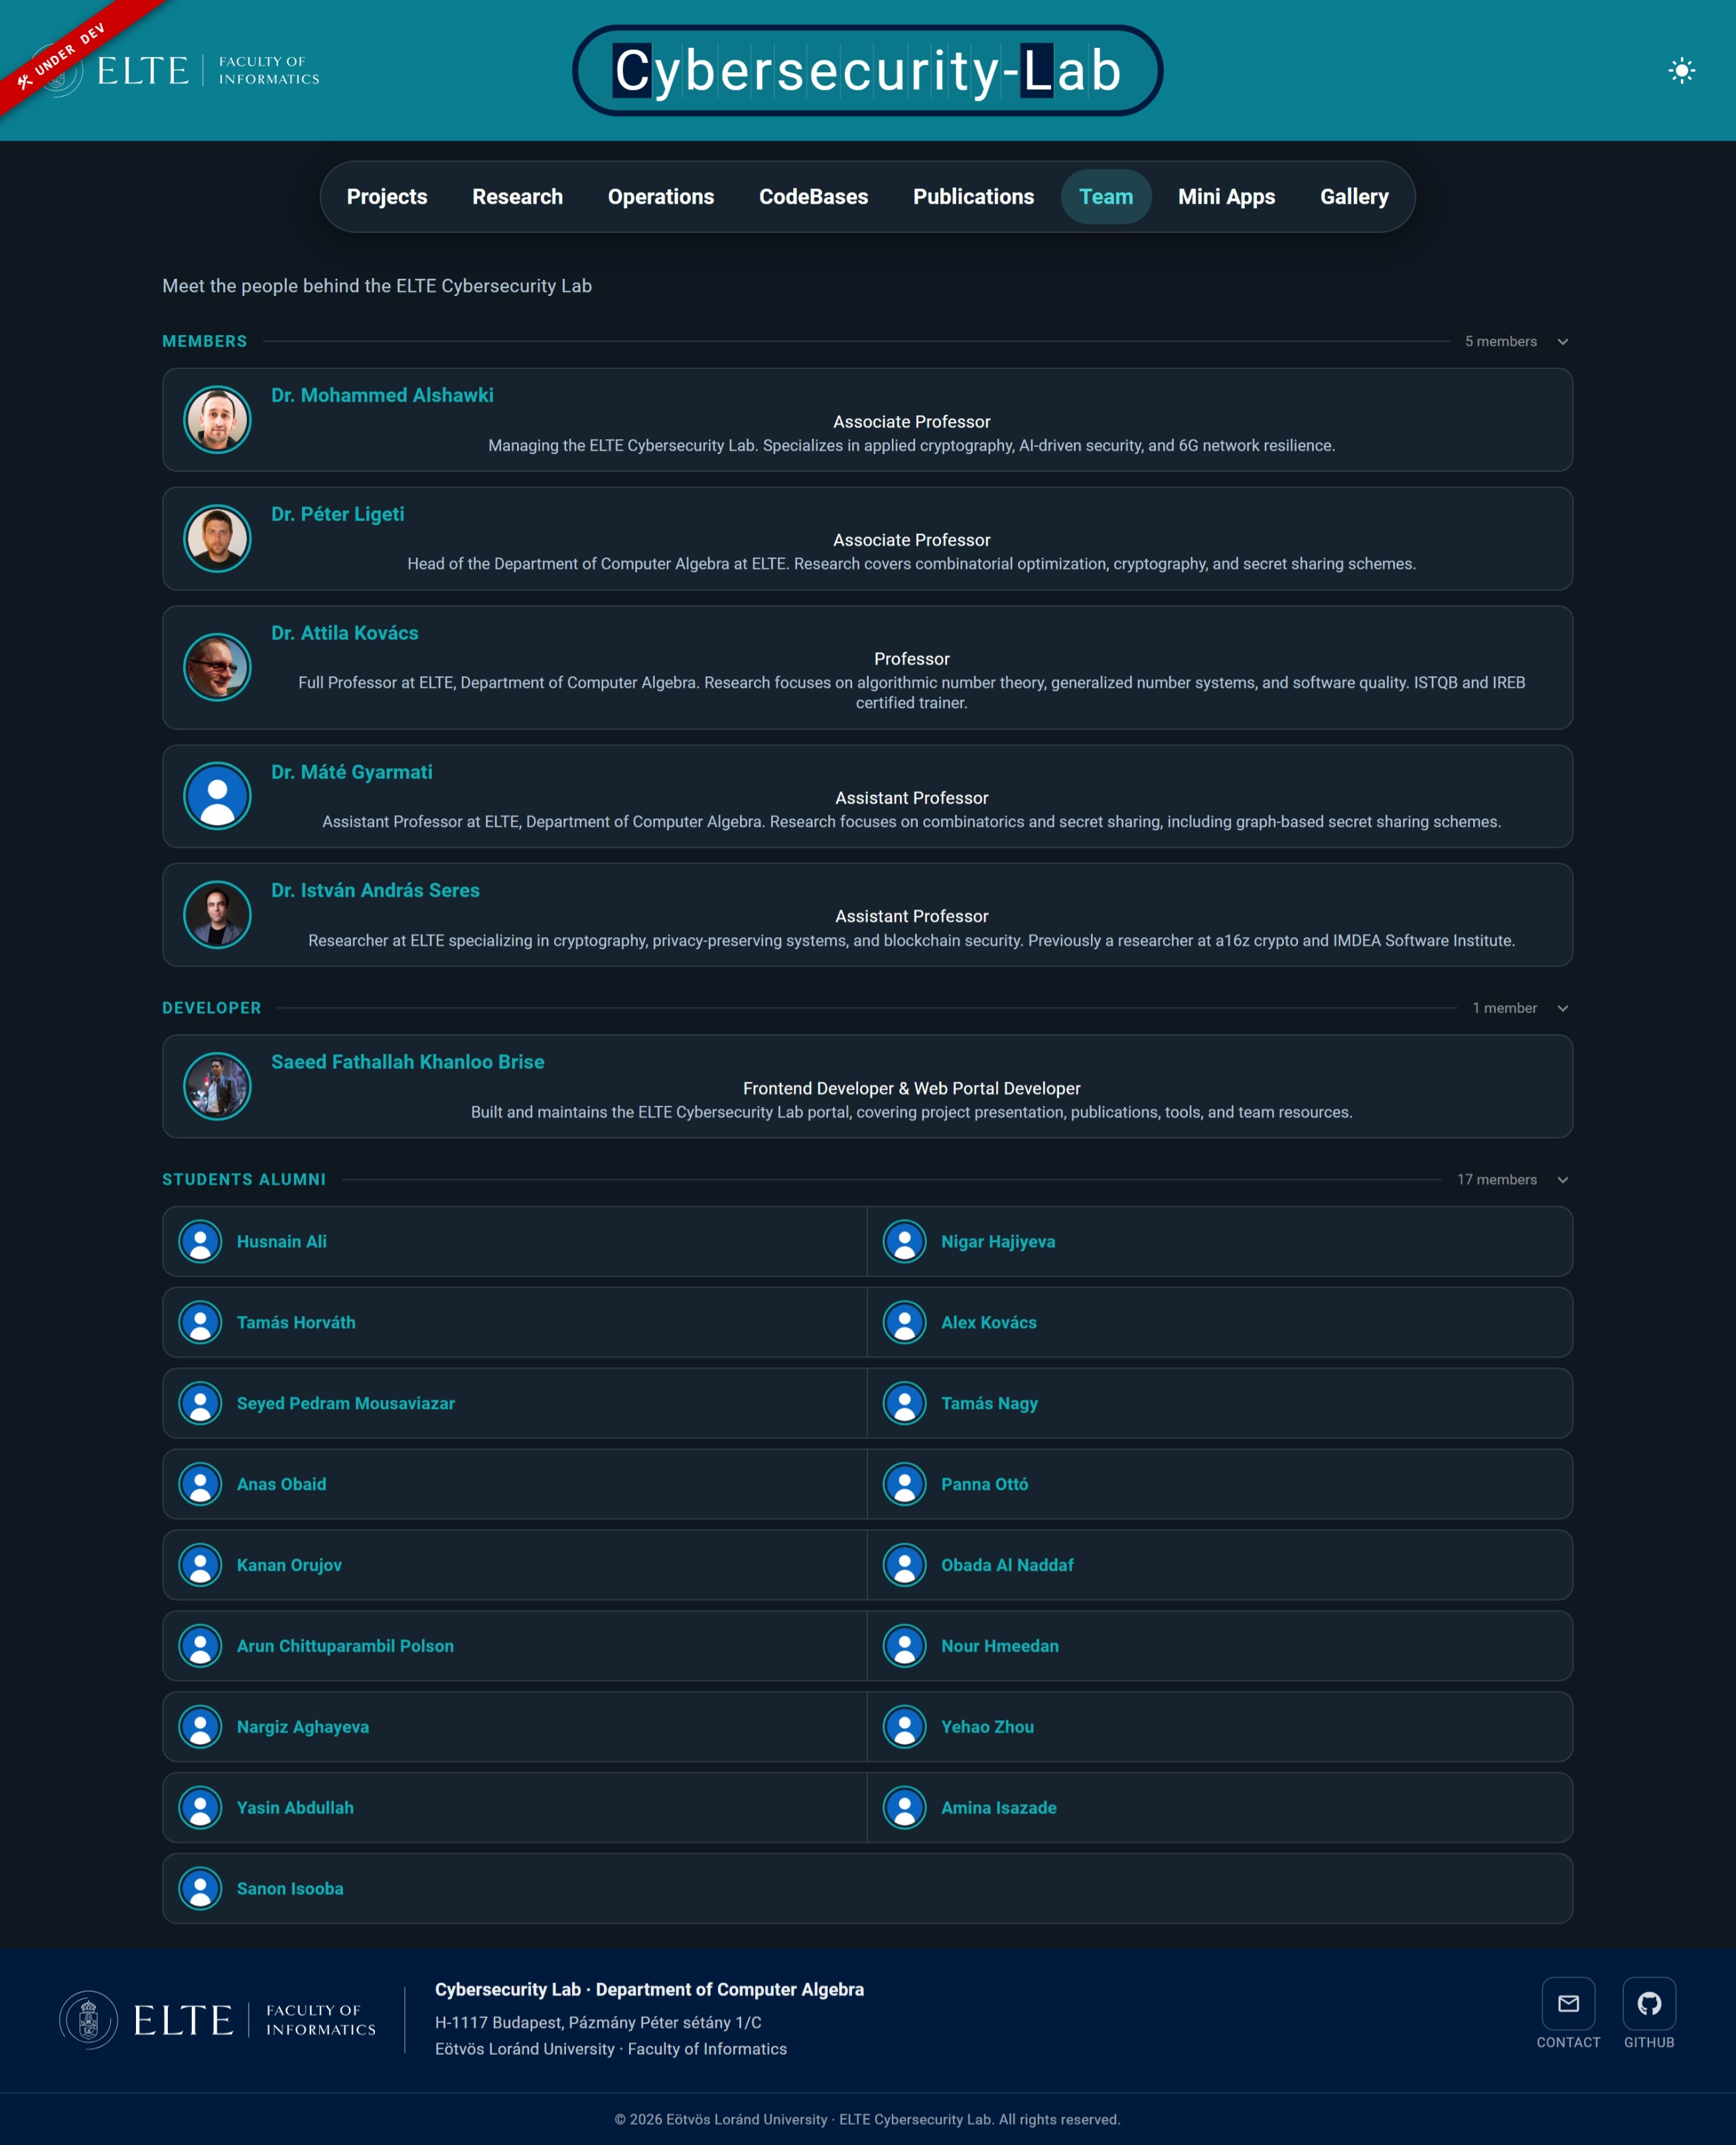
\includegraphics[width=0.88\textwidth]{images/team.jpeg}
	\caption{The Team page showing the Members, Developer, and Students Alumni categories. Members and Developer use the full card layout; alumni use the compact paired card layout on desktop.}
	\label{fig:team-page}
\end{figure}

\paragraph{Data file.} The Team page reads from \texttt{src/data/teamData.ts}. The file exports an array of \texttt{TeamCategory} objects, each with a \texttt{category} (the heading), and a \texttt{members} array. Each member has a \texttt{name}, \texttt{familyName}, \texttt{role}, \texttt{extraInfo}, \texttt{picture}, and \texttt{link}. The optional \texttt{title} field is for honorifics such as \textbf{Dr.} An empty \texttt{picture} field falls back to the default avatar. An empty \texttt{link} field renders the name as plain text instead of as a link.

The category order in the file is the category order on the page. Moving a member from one category to another is a matter of cutting and pasting the entry. Renaming a category renames its header. Adding a new category is a single new entry at the top level of the array.

%-----------------------------------------------------------
\section{Mini Apps Page}\label{sec:user-tools}

The Mini Apps page hosts the interactive tools and educational mini-applications built for the lab. At the time of writing there are two: \textbf{Ancient Cipher} and \textbf{Security Gauntlet}.

Each tool is shown as a card. The card has a square image at the top, two pill labels (a category label such as \textbf{Cryptography} or \textbf{Game}, and a status label such as \textbf{Live} or \textbf{Beta}), the tool's title, and a short description. Clicking the card opens the tool itself.

\textbf{Ancient Cipher} is a small encryption-and-decryption tool that supports classical ciphers (Caesar, Vigen{\`e}re). The visitor types in a message, picks a cipher, sets the cipher's parameters, and sees the encrypted or decrypted output update in real time. It is intended for teaching rather than for serious use; the goal is to give students an interactive way to play with the ciphers they read about in lectures.

\textbf{Security Gauntlet} is a collection of cybersecurity-themed mini-games, currently containing a Caesar cipher breakdown puzzle, a Keystone authentication packet-flow exchange, and a gradient defender game. The intent is for the gauntlet to grow over time as more games are added.

\begin{figure}[H]
	\centering
	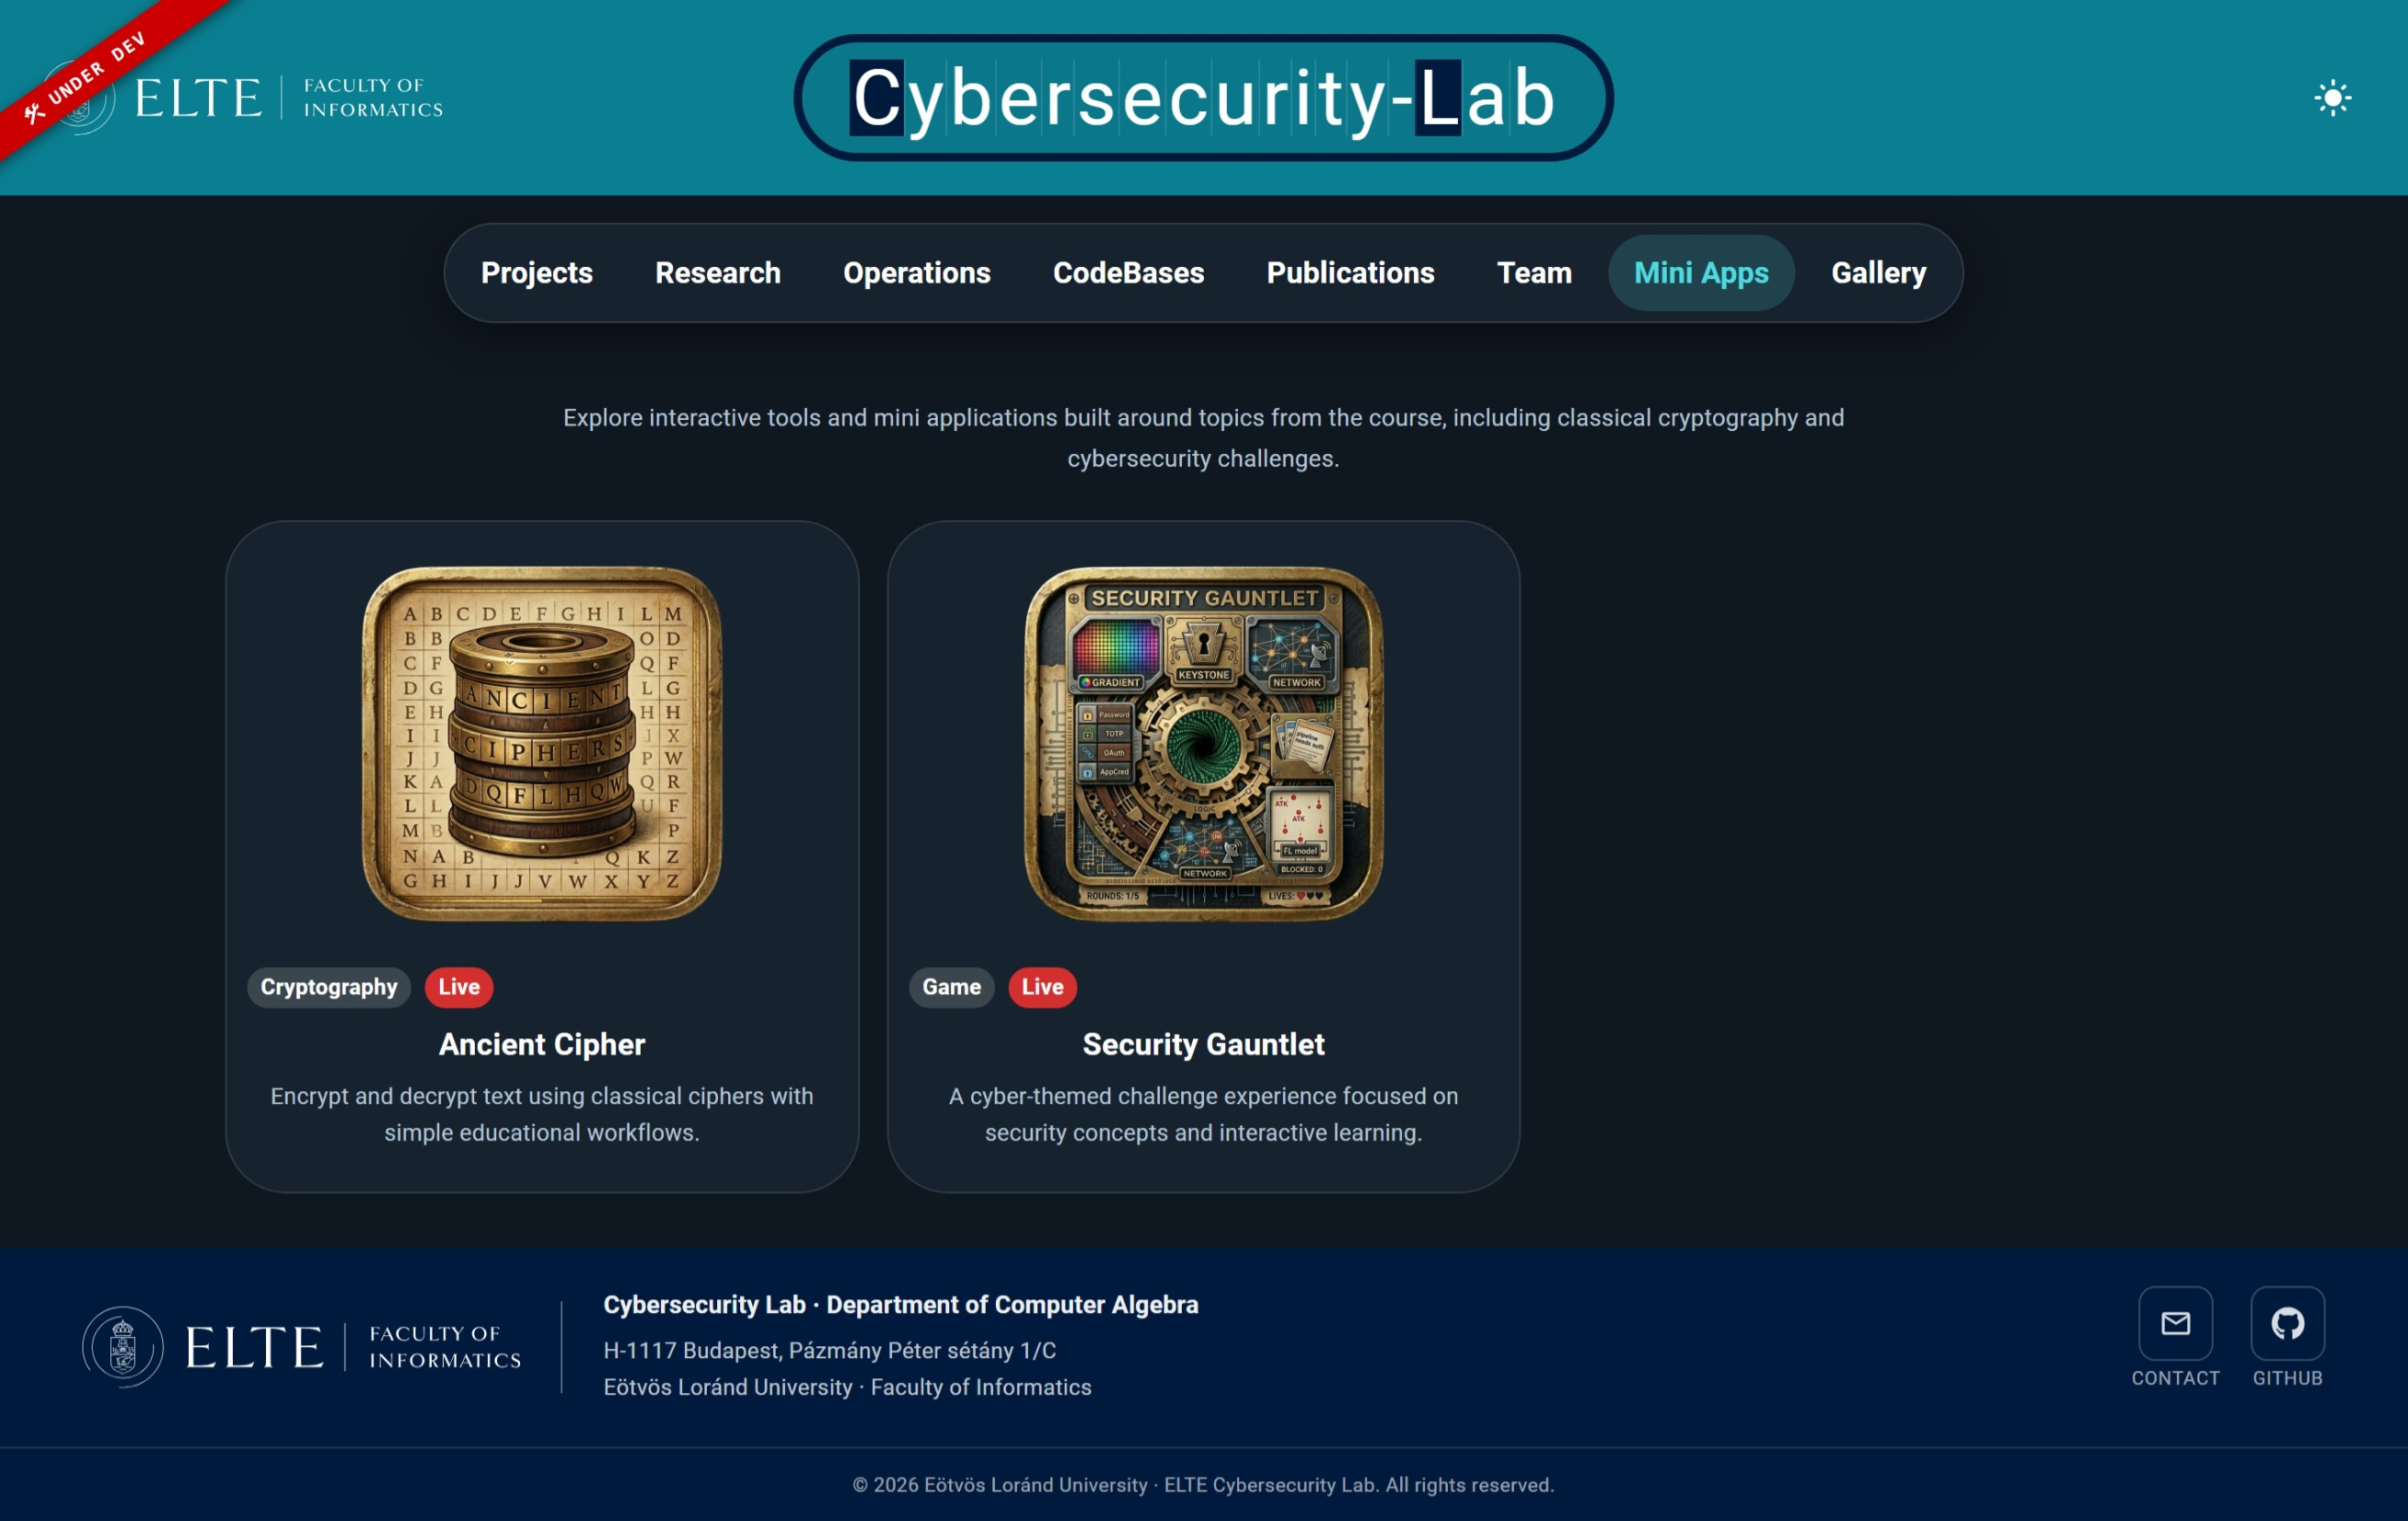
\includegraphics[width=0.78\textwidth]{images/mini-apps.jpeg}
	\caption{The Mini Apps page with two tool cards: Ancient Cipher (cryptography, live) and Security Gauntlet (game, live).}
	\label{fig:miniapps-page}
\end{figure}

\paragraph{Data file.} The Mini Apps page reads from \texttt{src/data/toolsData.ts}. Each tool entry has a \texttt{title}, \texttt{slug} (used as the route segment for the tool's page), \texttt{image} (a path to the card's image), \texttt{description}, optional \texttt{status} (\texttt{live}, \texttt{beta}, or \texttt{coming-soon}), and optional \texttt{category}. Adding a new tool requires the new entry in this file plus a route in the application that handles the tool's slug.

%-----------------------------------------------------------
\section{Gallery Page}\label{sec:user-gallery}

The Gallery page shows photographs of the lab, the university, and the campus. The photos are arranged onto stylised circuit-board-themed layouts, with three different board variants on desktop. The current layout shows the photo slot count at the top (e.g.\ \texttt{SECTION\_A // 04 SLOTS}) and arranges photos around drawn circuit traces with chip-like markers.

The visitor cycles through the available boards using the arrow controls on the sides of the layout. The pagination counter at the top of the page (e.g.\ \texttt{01 / 03}) shows the current board and the total. Clicking on any photo enlarges it for a closer look; clicking outside the enlarged photo collapses it back to the layout.

Three desktop board variants are available: a four-slot board (section A), and two three-slot boards (sections B and C). The portal picks a section for each page at random, with the constraint that the same section never appears twice in a row, so consecutive boards always use a different layout. If a section has more slots than the remaining photos provide, the empty slots are filled with the default photo so the board still looks complete. On mobile, the boards collapse to one photo per page to keep the layout readable on a narrow screen.

\begin{figure}[H]
	\centering
	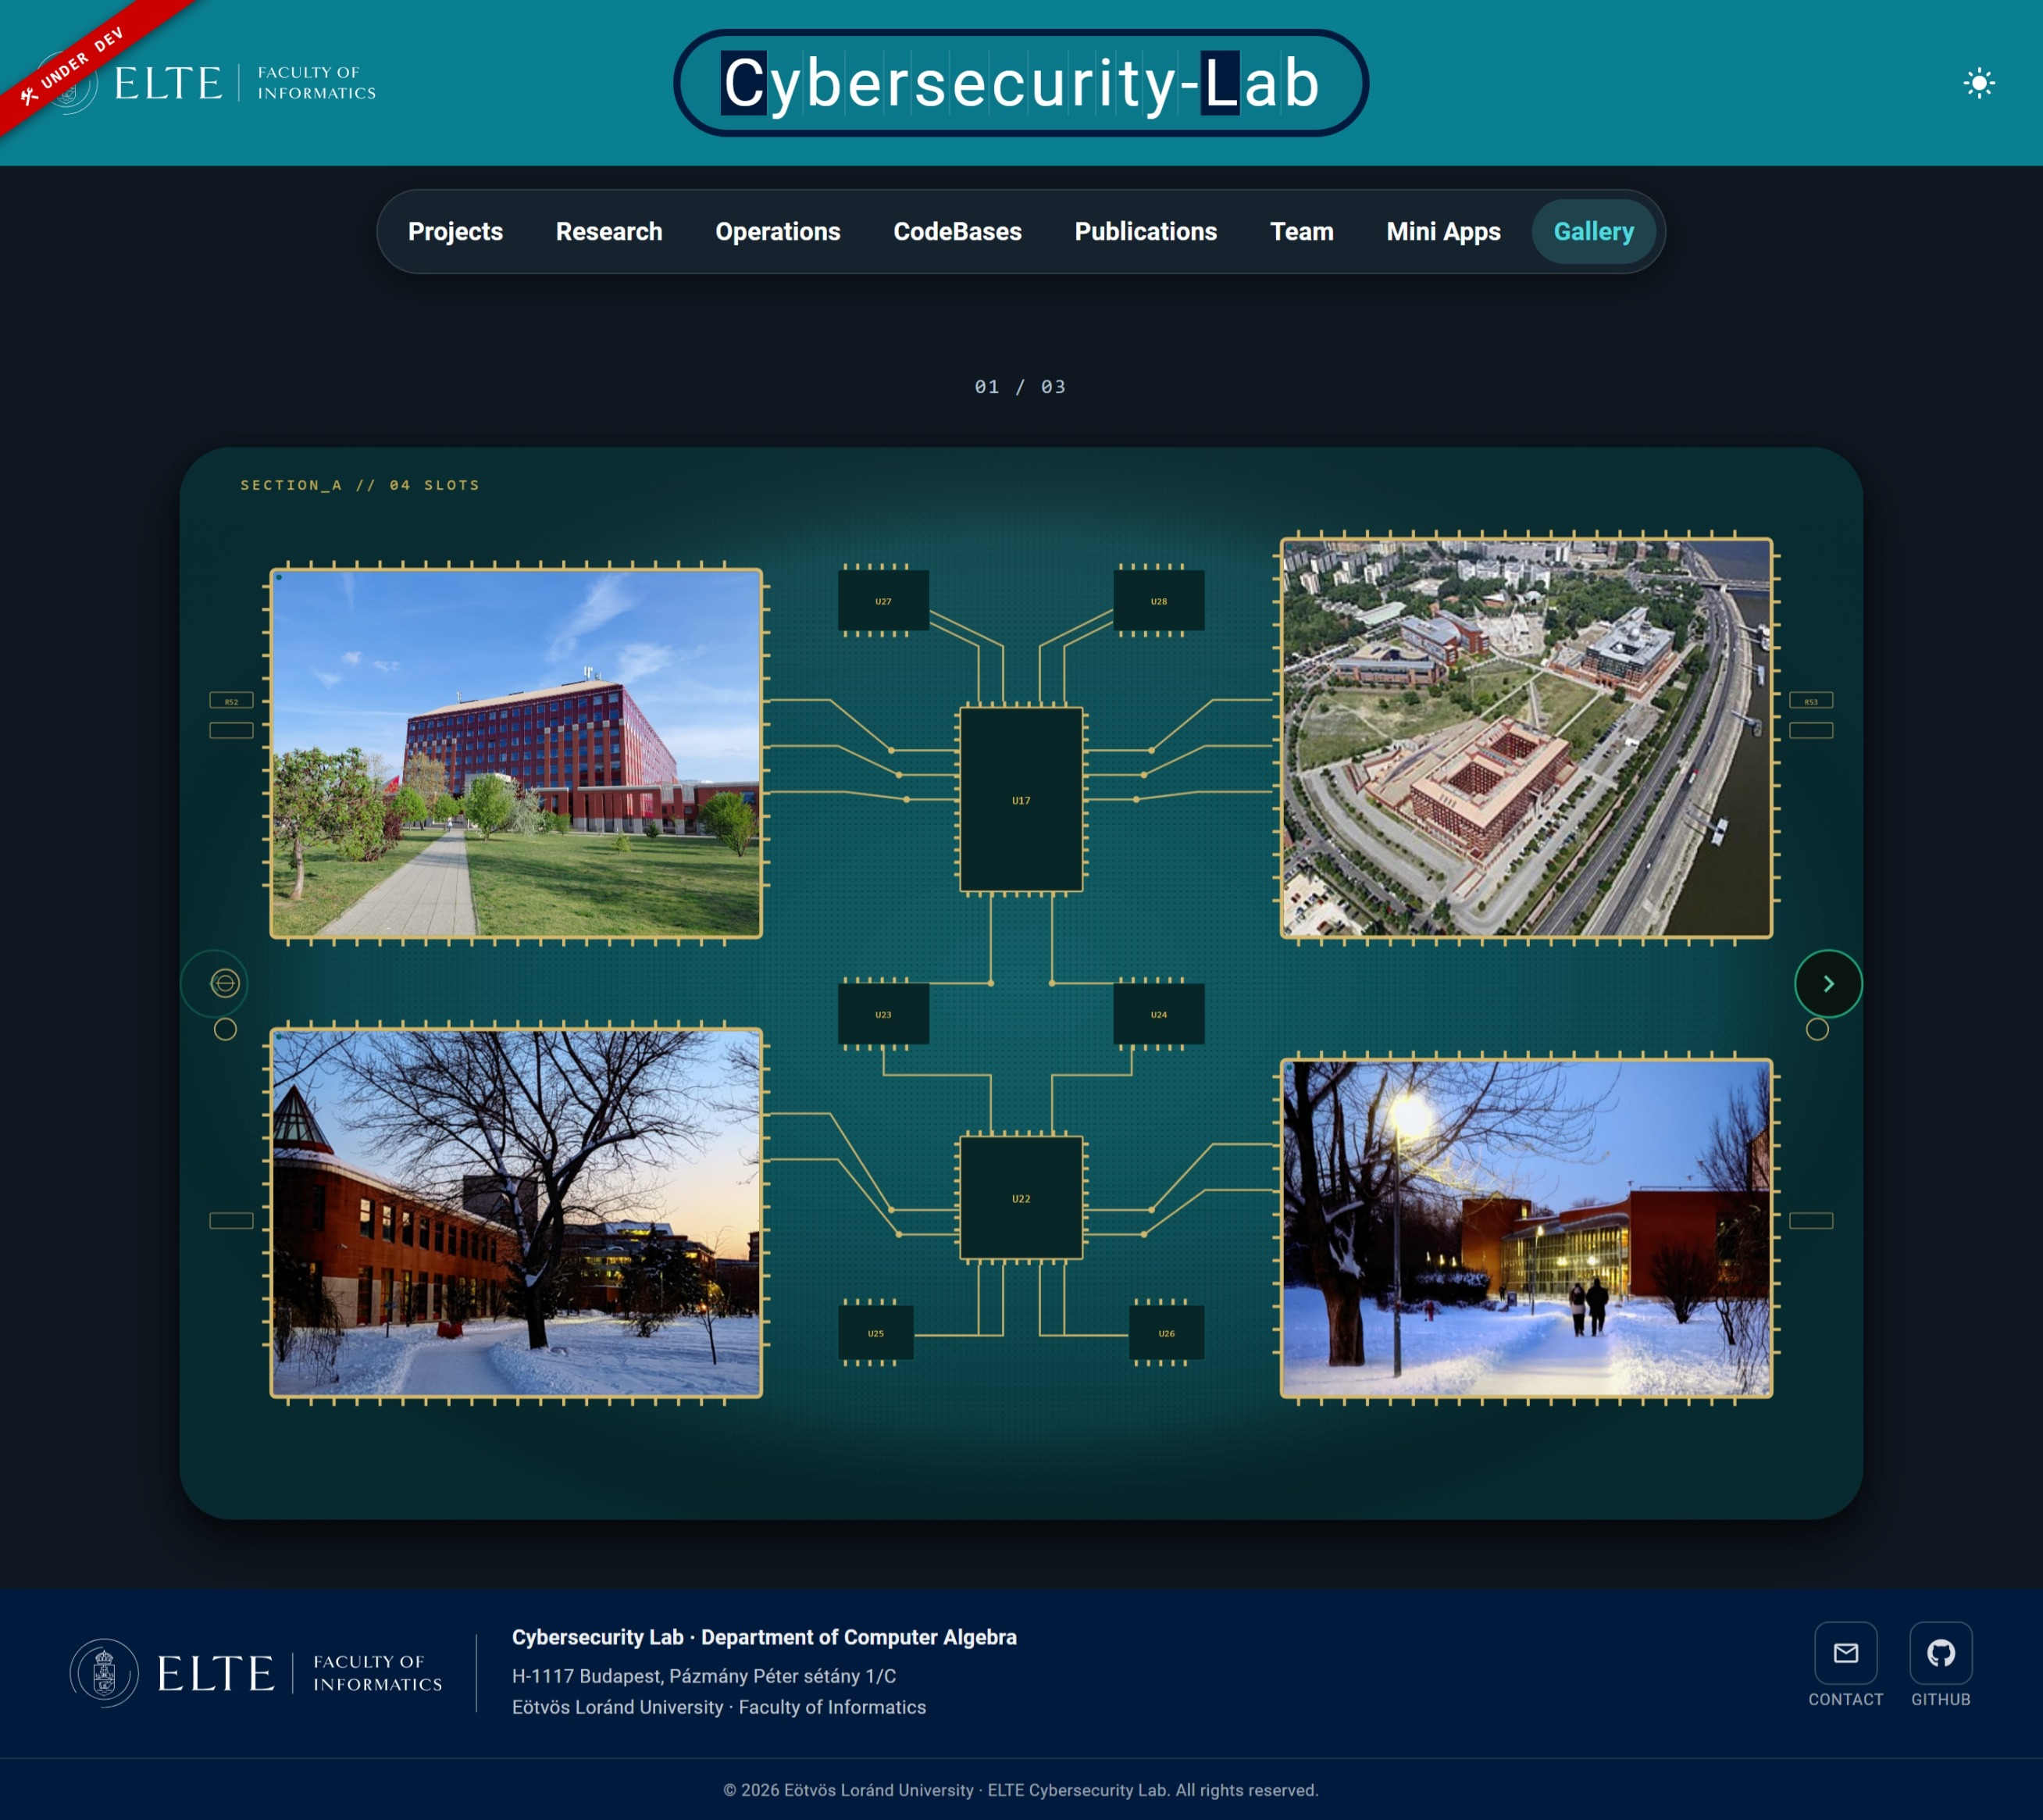
\includegraphics[width=0.88\textwidth]{images/gallery.jpeg}
	\caption{The Gallery page with a four-slot board (SECTION\_A) showing campus and lab photos arranged around drawn circuit traces. Arrow controls on the sides move to the next or previous board.}
	\label{fig:gallery-page}
\end{figure}

\paragraph{Data file.} The Gallery page reads from \texttt{src/data/galleryData.ts}. The file exports \texttt{galleryPhotos} (an array of file names), \texttt{defaultPhoto} (the file name used when a slot has no specific photo), and \texttt{galleryBasePath} (the directory where the photo files live in the \texttt{public/} folder). Adding photos is a matter of dropping the file into \texttt{public/gallery/} and adding its file name to the array. The portal handles the rest.

%-----------------------------------------------------------
\section{Contact Page}\label{sec:user-contact}

The Contact page is reachable from the \textbf{Contact} button in the footer rather than from the main navigation bar. It shows a single card titled \textbf{Contact} with a short paragraph (``Reach out for questions, collaboration, or general inquiries.''), an email line, and a phone line.

Below the contact details there is an \textbf{Open form} dropdown. Clicking it expands a contact form (name, email, message) inline below the contact card. The form is laid out but is not connected to a backend; submitting it does not currently send anything. The form is hidden behind the dropdown intentionally so that visitors who only want to copy the email or phone number do not have to scroll past an unused form.

The email and phone numbers shown on the page are currently placeholder values (\texttt{contact@example.com} and \texttt{+36 00 000 0000}). The lab is expected to replace these with the real values once they have decided what to publish.

\begin{figure}[H]
	\centering
	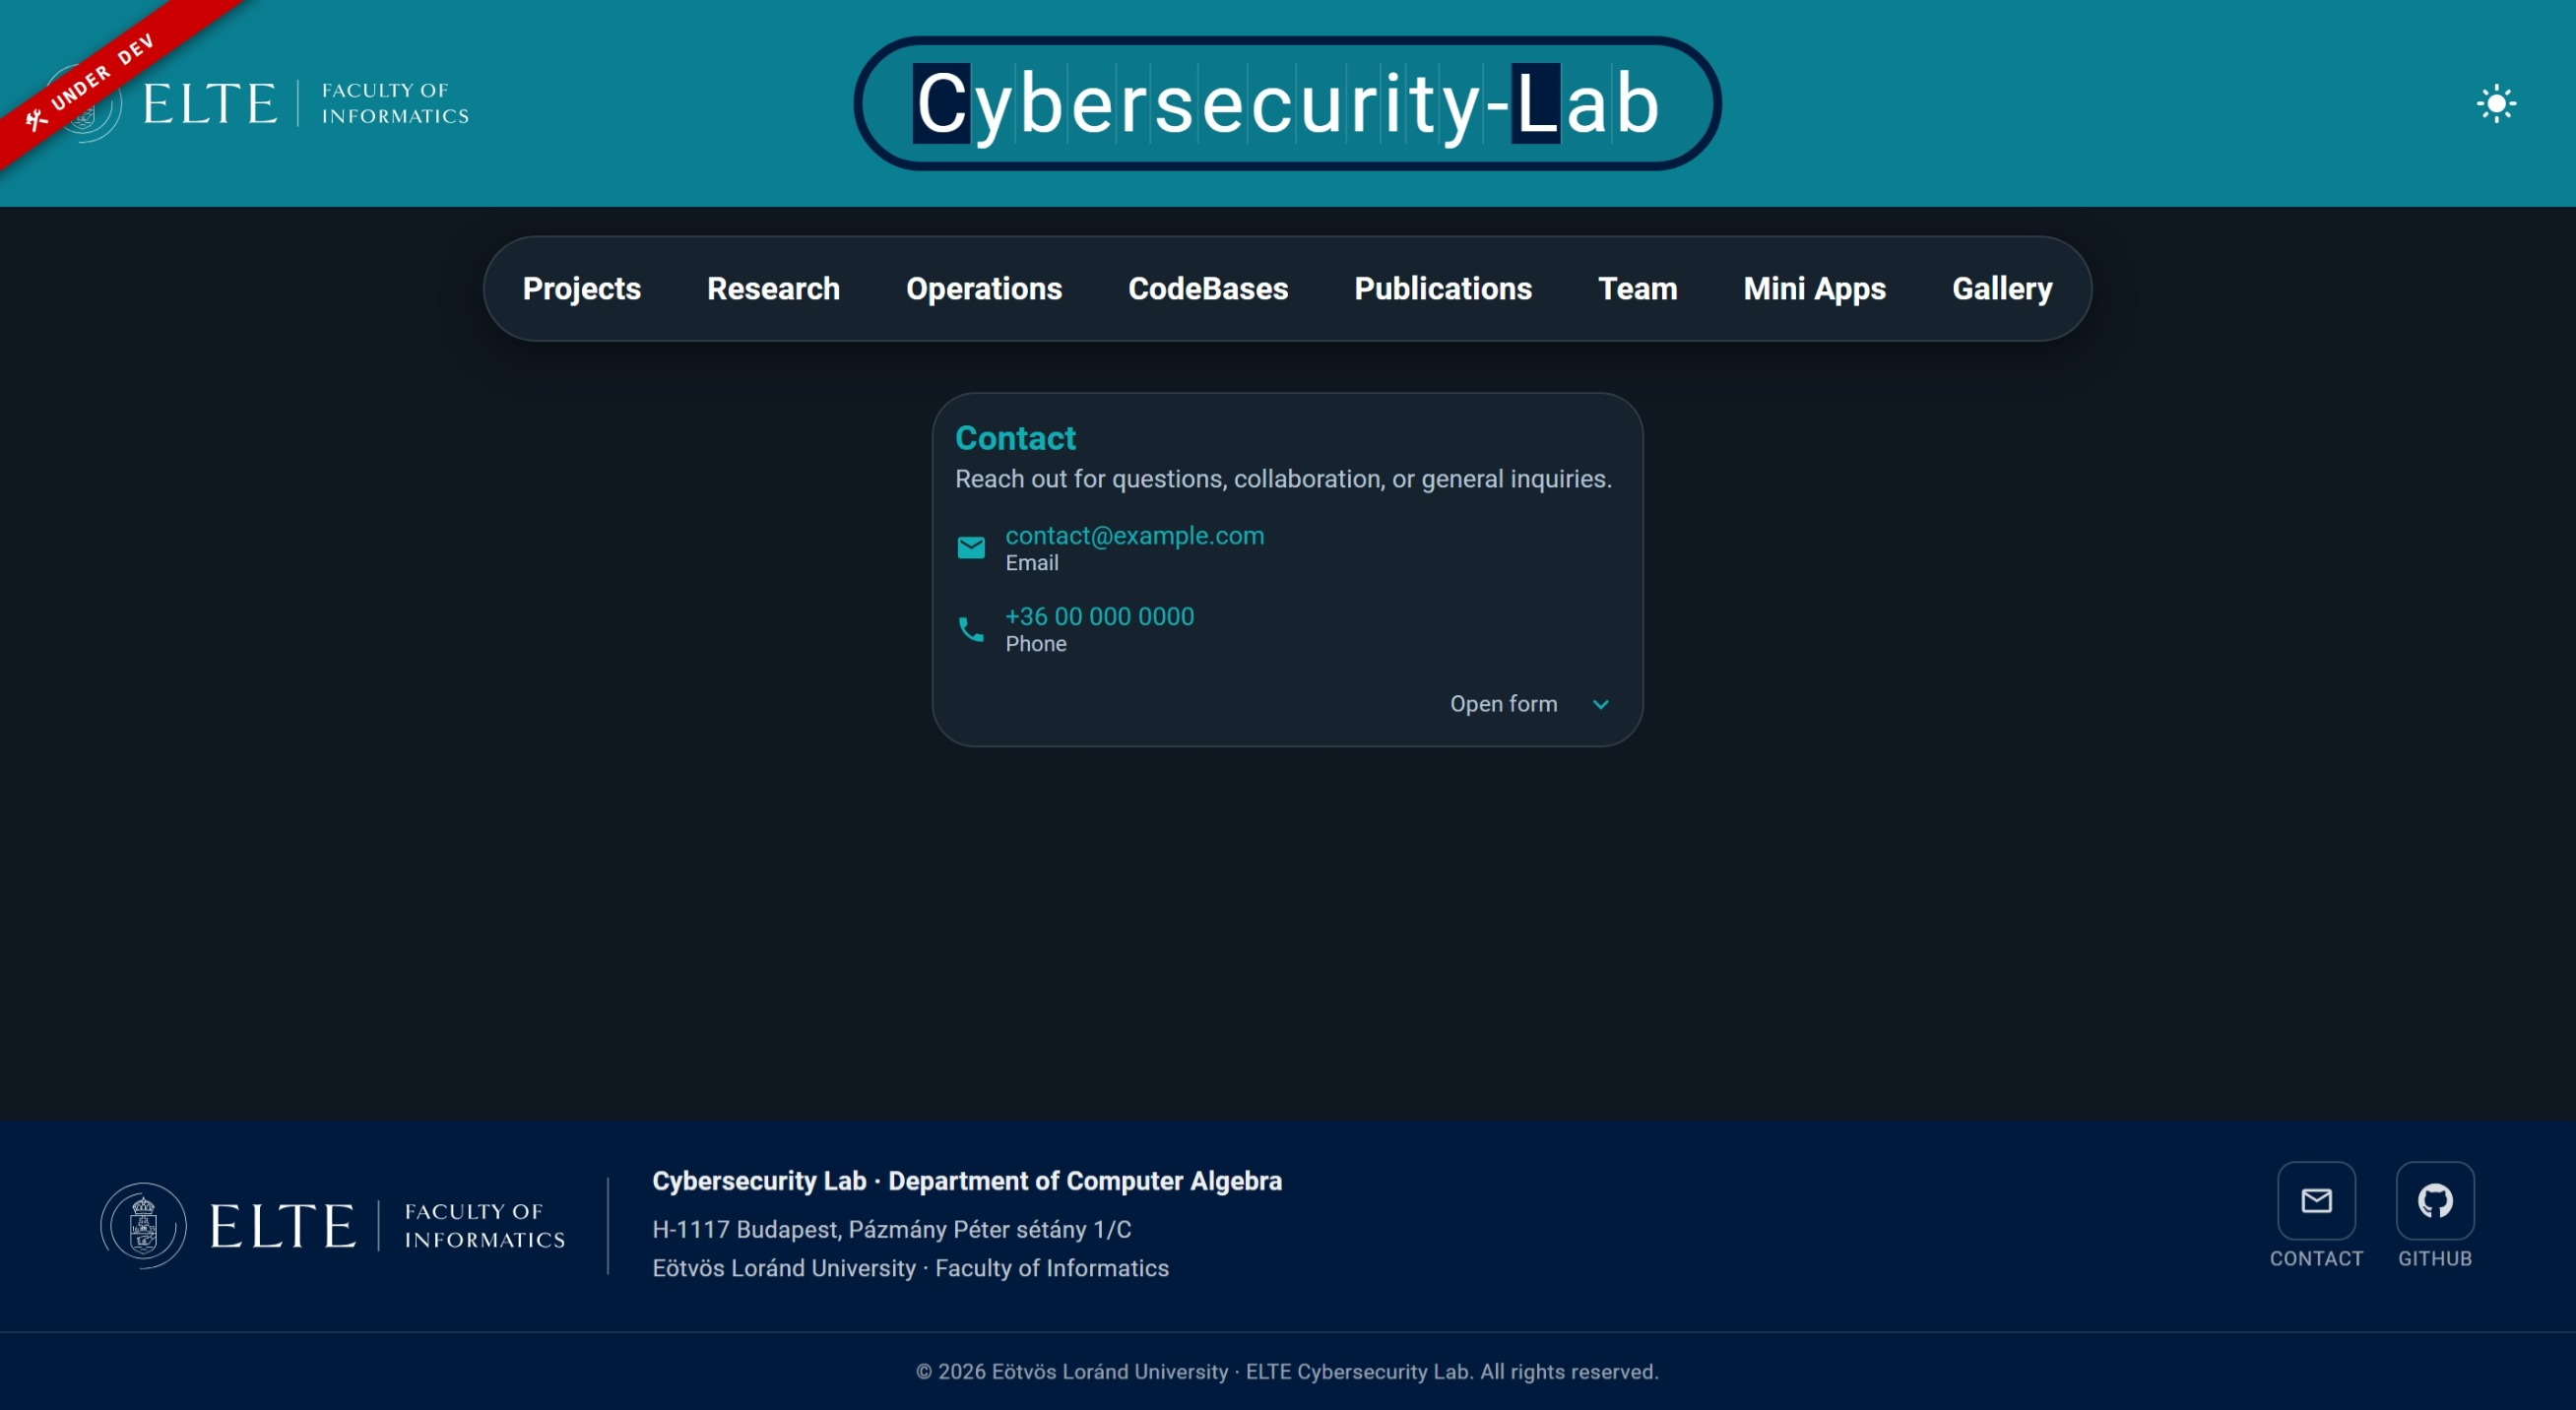
\includegraphics[width=0.88\textwidth]{images/contact-us.jpeg}
	\caption{The Contact page with the contact card showing the placeholder email and phone, and the Open form dropdown below for the contact form.}
	\label{fig:contact-page}
\end{figure}

\paragraph{Data file.} The Contact page reads from \texttt{src/data/contactPageData.ts}. The file is intentionally small: it has three fields, \texttt{email}, \texttt{phone}, and \texttt{showForm}. Setting \texttt{showForm} to \texttt{false} (the default) keeps the form behind the dropdown. Setting it to \texttt{true} would expand the form by default. The email and phone fields are plain strings.

%-----------------------------------------------------------
\section{GitHub Organisation Page}\label{sec:user-github}

The portal has a companion landing page on GitHub itself: the \texttt{profile/README.md} file in the \texttt{elte-cybersec/.github} repository, which GitHub renders as the organisation's profile page. This page is what visitors arriving through GitHub see first.

The GitHub organisation page mirrors the portal's structure rather than duplicating it. It has a waving banner at the top, an \textbf{About the lab} section, a \textbf{Research areas} grid with the same six areas as the Research page, a \textbf{Featured projects} grid with the lab's main public repositories, a \textbf{How we work} section that mirrors the Operations page, a \textbf{The team} section listing the lab manager and the scientific team, and \textbf{Get involved} and \textbf{Connect} sections that link back to the portal.

The intent is that visitors who arrive through GitHub do not have to leave GitHub to understand what the lab is about; they can read the organisation page and only follow the link to the portal if they want a more interactive experience. The two pages share the same brand colours and the same description text, so they feel like parts of the same identity. The top part of github page is shown in Figure~\ref{fig:github-org-page} on the next page.

\begin{figure}[H]
	\centering
	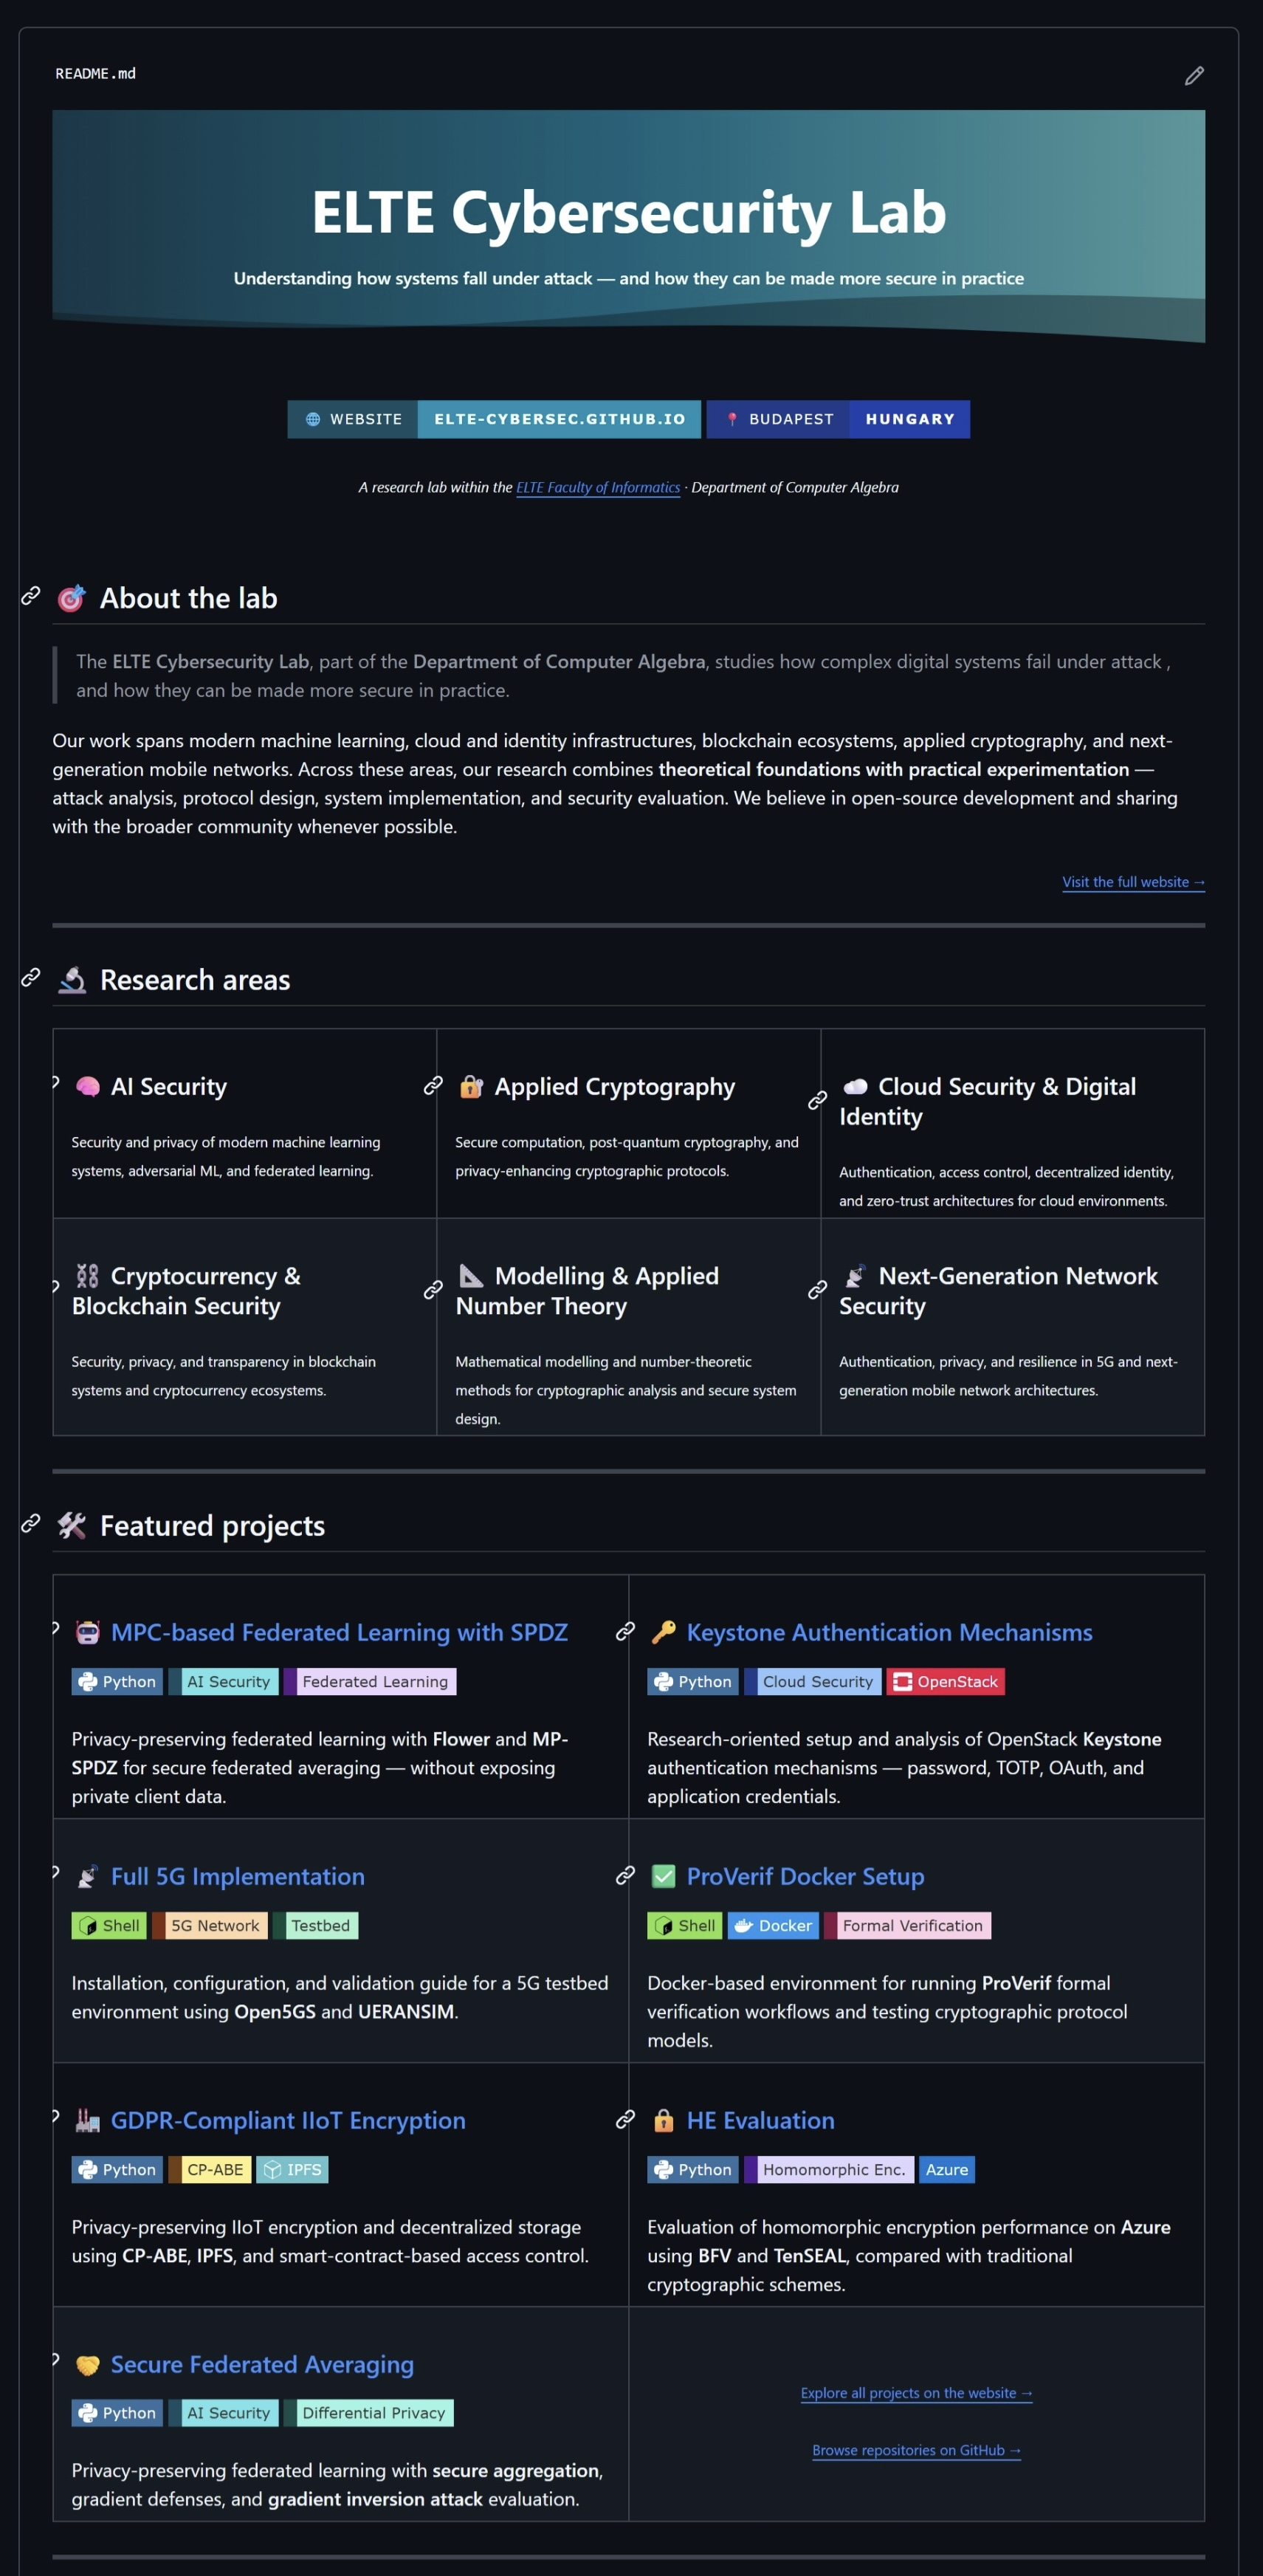
\includegraphics[width=0.75\textwidth]{images/github.jpeg}
	\caption{The ELTE Cybersecurity organisation page on GitHub, mirroring the structure of the portal with the about section, research areas, featured projects, how-we-work, team, and connect sections.}
	\label{fig:github-org-page}
\end{figure}
	\cleardoublepage
	
	%----------------------------------------------------------------------------
\chapter{Developer Documentation}\label{ch:dev}
%----------------------------------------------------------------------------

This chapter documents the portal from a developer's point of view. It opens with the technology stack, then describes the design decisions taken on each part of the portal and the alternative approaches that were considered and rejected. From there it moves into the architecture and the data flow, the parser that powers the CodeBases page, the pluggable component registry that powers the Operations principles, the theming and routing setup, and the project's repository layout. The chapter closes with a section on testing, since the testing performed during this project was manual and is short enough to belong here rather than in its own chapter.

%-----------------------------------------------------------
\section{Technology Stack}\label{sec:dev-stack}

The technology choices for the portal were practical rather than aspirational. The aim was a static, hostable-anywhere frontend with no backend dependency, so that the portal could be served from GitHub Pages without any infrastructure to maintain.

\subsection{Frontend Stack}\label{subsec:dev-stack-frontend}

\paragraph{React with TypeScript.}
React is the rendering library for the entire portal \cite{react}. TypeScript sits on top of React and types every component, every data file, and every utility \cite{typescript}. The data-driven architecture relies heavily on TypeScript: every page reads from one or more typed data files, and a typo in a field name or a wrong shape in a data file is caught at compile time rather than at runtime. The interfaces and types for each data file (\texttt{ResearchArea}, \texttt{ProjectRole}, \texttt{TeamCategory}, etc.) sit in the same data directory as the data, which keeps the type and the data near each other and makes it obvious to a future editor what shape an entry should have.

\paragraph{Vite.}
Vite is the build tool and development server \cite{vite}. It was picked for its fast cold start, fast hot reload, and small production bundle. The portal does not have a backend, so the entire production output is a static bundle that can be served by any static-file host. Vite produces that bundle through \texttt{npm run build}. Vite is also used to import the Markdown content files at build time through its \texttt{import.meta.glob} feature, which bundles every \texttt{.md} file in \texttt{src/content/} into the static output as a raw string.

\paragraph{React Router with Hash Routing.}
React Router handles client-side navigation between pages \cite{reactrouter}. The portal uses \texttt{HashRouter} rather than \texttt{BrowserRouter}, and the reason is GitHub Pages. GitHub Pages serves static files only; it does not run a server-side rewrite rule that would redirect every unknown URL back to \texttt{index.html}. With \texttt{BrowserRouter} this means deep links break: opening \texttt{example.com/projects} directly in the browser results in a 404, because there is no file at that path. With \texttt{HashRouter} the path lives after the \texttt{\#} (e.g.\ \texttt{example.com/\#/projects}), the actual file requested is always \texttt{index.html}, and the router handles the rest on the client. This makes shareable links to any page on the portal work reliably without any infrastructure tricks.

\paragraph{Material UI.}
Material UI supplies the base components: buttons, cards, dialogs, dropdowns, autocompletes, collapsibles, and the grid layout \cite{mui}. It uses Emotion for CSS-in-JS styling \cite{emotion}. The portal's brand colours, typography, and dark-and-light themes are configured through Material UI's theme provider, which means a theme change propagates to every Material UI component on the portal automatically.

\paragraph{Markdown rendering.}
The CodeBases page reads Markdown content from each repository's documentation file and renders it on the page. The Markdown is parsed with a Markdown parser and rendered through a React Markdown component, with custom renderers for headings, code blocks, tables, and images so that the rendered output picks up the portal's brand colours and dark-mode styling \cite{markdownit, reactmarkdown, commonmark}.

\subsection{Hosting and Automation}\label{subsec:dev-stack-hosting}

\paragraph{GitHub Pages.}
The portal is hosted on GitHub Pages \cite{githubpages}. The deployment pipeline is simple: Vite builds the static bundle into the \texttt{dist/} folder, and the contents of \texttt{dist/} are pushed to the \texttt{gh-pages} branch of the repository, which GitHub Pages serves. Because the portal has no backend, there is nothing else to deploy.

\paragraph{GitHub Actions.}
GitHub Actions is used (and where applicable, prepared) for automation \cite{githubactions}. There is one workflow for building and deploying the portal on push to the main branch, and there is a prepared (but not currently enabled) workflow that would fetch the latest documentation files from each tracked repository and commit the updated content back to the portal. The second workflow is disabled because it requires a GitHub access token to read the other lab repositories, and that token has not yet been provisioned for the project. The chapter on challenges and improvements describes this in more detail.

%-----------------------------------------------------------
\section{Design Decisions}\label{sec:dev-design}

This section explains the design decisions taken during the project. For each major decision, it describes the alternatives that were considered, what was eventually chosen, and why.

\subsection{Static Data Files Over a Backend}\label{subsec:dev-design-static}

The portal is a fully static client-side application. There is no API, no database, and no backend service. Every page reads its content from one or more TypeScript data files inside the \texttt{src/data/} directory at build time, and the resulting static bundle is what gets served to visitors.

The alternative would have been a small CMS or a custom backend with an admin panel. That was considered seriously, especially for the Publications page (which could grow into hundreds of entries) and the Team page (which changes whenever someone joins or leaves the lab). It was rejected for three reasons. The first is hosting: GitHub Pages does not run a backend, and the lab does not currently have infrastructure to host one. Adding a backend would mean either paying for a service, asking the university to host something, or running it on a personal server, and none of those was a good long-term option. The second is editing: a CMS adds an interface but it also adds an account, a database, and a deployment that all need to keep working. For a lab portal that changes weekly at most, that is a lot of moving parts. The third is the path of least resistance for the people who will actually edit the portal: opening a \texttt{.ts} file in a code editor and changing a string is faster than logging into a CMS, finding the right entry, editing it, saving it, and waiting for the cache to update.

The trade-off is that someone with no programming background cannot edit the portal without opening a code editor. That is acknowledged as a limitation and is discussed under improvements; a dedicated admin dashboard would be the right solution, but it requires the backend that was deliberately not built.

\subsection{Why Hash Routing}\label{subsec:dev-design-routing}

React Router supports two main routing modes: \texttt{BrowserRouter}, which uses the HTML5 history API and produces clean URLs like \texttt{/projects}, and \texttt{HashRouter}, which puts the path after a \texttt{\#} sign as in \texttt{/\#/projects}. The portal uses \texttt{HashRouter}, and the reason is purely a hosting constraint.

GitHub Pages is a static-file host. When a visitor opens \texttt{example.com/projects} directly, GitHub Pages looks for a file at \texttt{/projects} and, finding nothing, returns a 404. To make \texttt{BrowserRouter} work in this environment, the host has to be told to fall back to \texttt{index.html} for any unknown path, and GitHub Pages does not support that fallback. With \texttt{HashRouter}, the part after the \texttt{\#} is never sent to the server, so the request is always for the root of the site, GitHub Pages always returns \texttt{index.html}, and the router takes the path from the hash on the client.

Clean URLs would have been nicer to look at, but they would have required either moving to a different host (Vercel, Netlify, or a custom server) or accepting that direct links to pages would not work. Neither was worth it for a portal whose main user journey is to land on the home page and click through the navigation bar.

\subsection{Structured Markdown for CodeBases}\label{subsec:dev-design-markdown}

The CodeBases page was the first page where the data-driven design was forced to deal with content that was not under the portal's direct control: documentation files written by the people who own the repositories. Three approaches were considered.

The first approach was to render each documentation file exactly as GitHub renders a README, in one long scroll, with no internal navigation. That was the first version that got built. It looked acceptable for one repository and broke down completely as soon as there were several, because each document has a different shape, a different length, and a different idea of what belongs where. There was no chapter-like feel and no way to navigate inside a project.

The second approach was to ignore the README entirely and store all the documentation content inside the portal as separate files or data structures. That was rejected because it would duplicate work: the repository owner would have to maintain the documentation on GitHub for the repository's own visitors, and again on the portal for the portal's visitors. Any change would have to be made twice. Duplication is the kind of thing that breaks down the fastest.

The third approach, the one that was taken, was to fix the document shape rather than the rendering. A simple convention was agreed: one first-level heading for the repository title, second-level headings for top-level topics, third-level headings for sub-topics. With that convention in place, a parser can take any document that follows it and split it into navigable topics. The repository owner maintains a single document, the portal reads that document at build time, and the page renders it as a course-like walkthrough. A template Markdown file is included with the project so that any new repository can copy it and follow the same shape from the start.

A small metadata block at the top of each document (a \texttt{\#\# PORTAL\_METADATA} heading followed by a \texttt{portal} fenced code block) carries the fields the portal needs to render the card on the CodeBases page (title, summary, logos, repository URL, dates). Keeping the metadata in the same file as the content means everything about a repository lives in one place: open one file and you see both the card description and the topics that will appear on the detail page.

\subsection{Pluggable Components on the Operations Page}\label{subsec:dev-design-pluggable}

The principles section of the Operations page presents an interesting design problem. Each principle has a written description on one side and an interactive visual on the other. The visuals are not generic icons; they are custom SVG-and-React components, each illustrating something specific about the principle. The question was how to bind a principle (which lives in the data file) to its visual (which is a React component).

The naive approach is to put the component reference directly into the data file. That was rejected because data files should not import React components; it would push the data into needing to know about the rendering layer, and it would mean that anyone editing the data has to import the right component and remember the right name.

The approach taken was a small registry. Each principle in the data file declares a \texttt{componentKey} string and an \texttt{iconFallback} string. The page keeps a registry that maps component keys to actual React components. At render time, the page looks up the key. If a component is registered for that key, it is rendered. If not, the fallback (a Material UI icon name) is rendered instead.

This decouples the data from the components in both directions. Adding a new principle whose visual already exists in the registry requires no code changes at all; only a new entry in the data file. Adding a new visual requires one new component file and one line in the registry, after which it is available to every principle in the data file. The fallback means the page never breaks: if the data file references a key that does not exist, the icon shows up instead and the rest of the page still renders.

\subsection{Interaction Pattern: Click-to-Expand}\label{subsec:dev-design-interaction}

Three of the lab's biggest pages (Projects, Research, Operations) share the same interaction pattern: a graphical element on the page (a node graph, a honeycomb, a quadrant grid), and clicking an item in the graphic opens a detail panel either next to it or below it on smaller screens. This was an intentional choice. The first interactive page built was the Research honeycomb, and once that was working the same pattern was applied to the other two for consistency. A visitor who has used the honeycomb on the Research page already knows how to use the role grid on the Operations page and the project graph on the Projects page; they do not have to learn a new interaction.

The one place where the pattern is deliberately not followed is the Projects page, where the first project is auto-selected on page load. This is because the Projects page is the entry point for most visitors interested in research output, and showing nothing on page load would force them to click before they could read anything. The Research and Operations pages, by contrast, are introductory in nature; their job is to give an overview first and the details only on demand.

\subsection{Why a Decoded-Text Header}\label{subsec:dev-design-header}

The portal title in the header (\textbf{Cybersecurity-Lab}) is animated: on every page load, it appears as a scrambled string of characters and then resolves into the readable title over a second or so. This is a small touch and could easily have been left out. It was kept because it fits the lab's identity, the lab studies cryptography, authentication, and systems that hide and reveal information, and a small decoded-text animation in the header echoes that. The animation runs once per load and does not repeat, so it does not become annoying.

\subsection{Why Layout Diversity in the Gallery}\label{subsec:dev-design-gallery}

The Gallery page picks one of three different board layouts for each page of photos. The alternative would have been a single, fixed layout. The reason a varied pick was preferred is honesty about the photo set: the lab does not have a fixed number of curated photos, and the photo set is expected to grow over time. A fixed layout would have to be designed for a specific photo count, and adding photos would require redesigning the page. Three layouts that handle different photo counts means new photos can be added without changing the page; the portal picks a layout that fits and rotates between them so the same section does not appear twice in a row.

\subsection{Why No Image Generation for Visuals}\label{subsec:dev-design-visuals}

Several of the visual elements on the portal (the honeycomb, the role grid, the interactive principle components, the project node graph) could have been done with rendered images or external illustrations. Instead they are all built as SVG inside React components.

The trade-off was deliberate. SVG components scale to any screen size without loss of quality, they pick up the theme colours through CSS variables, and they animate cleanly with browser primitives. An exported image would have looked good at one size, broken at others, and required a re-export every time a theme colour or a small detail changed. For interactive elements specifically, SVG-in-React is also much easier to wire up to click and hover handlers than an image would be.

The cost is that the components are more work to build than dropping an image into the page would have been. That cost was paid once per component and is not paid again.

%-----------------------------------------------------------
\section{Architecture and Data Flow}\label{sec:dev-architecture}

The portal's architecture is intentionally flat. There is no state management library, no global store, no event bus, no service layer. Each page is a self-contained React component that imports its data from one or more files in \texttt{src/data/}, applies its own internal state (which project is selected, which category is expanded), and renders.

The flow for a typical page is straightforward: the page component imports its data file at the top, types the import using the interfaces exported from the data file itself, and then iterates over the data to render the page. Selection state (which hex is open, which role is selected) lives in the page component's local state and resets when the visitor navigates away. There is no caching layer because there are no asynchronous fetches; every piece of data is bundled into the static output and available synchronously.

Asset paths across the portal are routed through a small utility, \texttt{resolveAssetPath}. Because the portal is served from a sub-path on GitHub Pages, every image and avatar URL needs the right base prefix to resolve correctly. The utility handles this in one place so that components do not have to: it returns external URLs unchanged, leaves \texttt{data:} URLs alone, and prefixes relative paths with Vite's \texttt{BASE\_URL}. Listing~\ref{lst:asset-path} shows it in full.

\begin{lstlisting}[language=TypeScript,caption={\texttt{resolveAssetPath} utility used by every component that renders an image, avatar, or logo.},label={lst:asset-path}]
	const DEFAULT_PREFIX = import.meta.env.BASE_URL;
	
	export function resolveAssetPath(path?: string | null): string {
		if (!path) {
			return DEFAULT_PREFIX;
		}
		
		if (/^(https?:)?\/\//i.test(path) || path.startsWith("data:")) {
			return path;
		}
		
		const normalizedPath = path.startsWith("/") ? path.slice(1) : path;
		
		return `${DEFAULT_PREFIX}${normalizedPath}`;
	}
\end{lstlisting}

%-----------------------------------------------------------
\section{The CodeBases Parser}\label{sec:dev-parser}

The CodeBases parser is the most involved piece of code in the project. It takes a raw Markdown string and produces a structured representation that the documentation view can render as a navigable course. It also pulls out a small metadata block embedded near the top of the document, which the CodeBases card on the index page uses.

\subsection{Loading the Documents}\label{subsec:dev-parser-loading}

The Markdown files live in \texttt{src/content/} and are loaded at build time by Vite. The portal does not fetch them at runtime; the loader reads every \texttt{.md} file in the directory and bundles it into the static output as a raw string. Listing~\ref{lst:repo-loader} shows the loader.

\begin{lstlisting}[language=TypeScript,caption={\texttt{getRepositoryPages} loads every Markdown file from \texttt{src/content/} as a raw string at build time.},label={lst:repo-loader}]
	import type { RepositoryPageMeta } from "../types";
	
	export function getRepositoryPages(): RepositoryPageMeta[] {
		const modules = import.meta.glob("../content/*.md", {
			eager: true,
			query: "?raw",
			import: "default",
		}) as Record<string, string>;
		
		return Object.entries(modules).map(([filePath, content]) => {
			const fileName = filePath.split("/").pop() ?? "";
			const fileSlug = fileName.replace(/\.md$/i, "");
			
			return {
				fileName,
				fileSlug,
				content,
			};
		});
	}
\end{lstlisting}

The file slug (the file name without its extension) is the default identifier for a repository if the metadata block does not supply one of its own. Once the raw content is loaded, each document is handed to the parser.

\subsection{The Document Parser}\label{subsec:dev-parser-document}

The parser walks the Markdown line by line and identifies headings, the table of contents, the metadata block, and code fences. It treats the first \texttt{\#} heading as the document title, \texttt{\#\#} headings as sections, and \texttt{\#\#\#} headings as sub-sections (called children of a section). A \texttt{\#\# Table of Contents} heading and the lines underneath it are skipped, because the portal builds its own sidebar from the section list and the in-document table of contents would only duplicate that. A \texttt{\#\# PORTAL\_METADATA} heading marks the start of the metadata block, which is read separately and not added to the rendered content.

A small \texttt{slugifyHeading} helper turns each heading title into a stable identifier the sidebar can use as a URL fragment and as a React key. Listing~\ref{lst:slugify} shows it.

\begin{lstlisting}[language=TypeScript,caption={\texttt{slugifyHeading} converts a heading title into a stable identifier.},label={lst:slugify}]
	function slugifyHeading(title: string): string {
		return title
		.toLowerCase()
		.replace(/[`*_~]/g, "")
		.replace(/[^\p{L}\p{N}\s-]/gu, "")
		.trim()
		.replace(/\s+/g, "-");
	}
\end{lstlisting}

The core of the parser is a state machine over the lines of the document. It keeps the current section, the current child, two buffers for accumulating the body of each, and a few flags that track whether the walker is currently inside a code fence, the table of contents, the metadata block, or the metadata's fenced code.

The first half of the walk, shown in Listing~\ref{lst:parser-core-1}, handles the special states: the metadata block, the \texttt{\#\# PORTAL\_METADATA} marker, and code fences. These checks come first because they all suppress normal content handling for the lines they cover.

\begin{lstlisting}[language=TypeScript,caption={The first half of \texttt{parseRepositoryDocument}: special-state handling for metadata, the portal block, and code fences.},label={lst:parser-core-1}]
	for (const rawLine of lines) {
		const trimmedLine = rawLine.trim();
		
		if (insideMetadata) {
			if (!insidePortalBlock) {
				if (trimmedLine.startsWith("```portal")) {
					insidePortalBlock = true;
				}
				continue;
			}
			
			if (trimmedLine === "```") {
				metadata = parsePortalMetadataBlock(portalBlockLines);
				insidePortalBlock = false;
				insideMetadata = false;
				continue;
			}
			
			portalBlockLines.push(rawLine);
			continue;
		}
		
		if (trimmedLine === "## PORTAL_METADATA") {
			flushSection();
			insideTableOfContents = false;
			insideMetadata = true;
			continue;
		}
		
		if (isFenceLine(rawLine)) {
			insideCodeFence = !insideCodeFence;
			if (!insideTableOfContents) {
				pushContentLine(rawLine);
			}
			continue;
		}
		
		if (insideCodeFence) {
			if (!insideTableOfContents) {
				pushContentLine(rawLine);
			}
			continue;
		}
	\end{lstlisting}
	
	The second half, shown in Listing~\ref{lst:parser-core-2}, handles the headings themselves and the fall-through case for regular content lines. A \texttt{\#\#} heading whose title matches ``Table of Contents'' switches the walker into TOC mode (which suppresses content until the next \texttt{\#\#}); a \texttt{\#} heading is the document title and is skipped; a \texttt{\#\#} heading starts a new section; a \texttt{\#\#\#} heading starts a new child of the current section.
	
	\begin{lstlisting}[language=TypeScript,caption={The second half of \texttt{parseRepositoryDocument}: heading handling and fall-through to content lines.},label={lst:parser-core-2}]
		const headingMatch = rawLine.match(/^(#{1,3})\s+(.*)$/);
		
		if (headingMatch) {
			const level = headingMatch[1].length;
			const title = headingMatch[2].trim();
			
			if (level === 2 && /table of contents/i.test(title)) {
				flushSection();
				insideTableOfContents = true;
				continue;
			}
			
			if (insideTableOfContents) {
				if (level === 2) {
					insideTableOfContents = false;
				} else {
					continue;
				}
			}
			
			if (level === 1) {
				continue;
			}
			
			if (level === 2) {
				startNewSection(title);
				continue;
			}
			
			if (level === 3) {
				startNewChild(title);
				continue;
			}
		}
		
		if (insideTableOfContents) {
			continue;
		}
		
		pushContentLine(rawLine);
	}
	
	flushSection();
\end{lstlisting}

A few details are worth flagging. The code fence detection is what stops the parser from treating a \texttt{\#\#} heading inside a code block as a real section heading. The \texttt{flushSection} helper finalises the current section (closing its child if any), commits it to the section list, and resets the buffers. The fallback for unparseable lines (in the surrounding \texttt{try/catch}, not shown here) writes a short warning into the section body so the document still renders even if a single line trips up the walker.

\subsection{The Metadata Block}\label{subsec:dev-parser-metadata}

The metadata block uses a deliberately simple format: \texttt{key: value} lines inside a \texttt{portal} fenced code block, with a special \texttt{logos:} key that introduces a list of dash-prefixed entries. Listing~\ref{lst:metadata-parser} shows the helper that reads it.

\begin{lstlisting}[language=TypeScript,caption={\texttt{parsePortalMetadataBlock} reads the small key/value block at the top of each document.},label={lst:metadata-parser}]
	function parsePortalMetadataBlock(lines: string[]): ParsedPortalMetadata {
		const metadata: ParsedPortalMetadata = {};
		const logos: string[] = [];
		
		let insideLogos = false;
		
		for (const rawLine of lines) {
			const line = rawLine.trim();
			
			if (!line) continue;
			
			if (line.startsWith("logos:")) {
				insideLogos = true;
				continue;
			}
			
			if (insideLogos && line.startsWith("-")) {
				logos.push(line.replace(/^-+\s*/, "").trim());
				continue;
			}
			
			if (insideLogos && !line.startsWith("-")) {
				insideLogos = false;
			}
			
			const separatorIndex = line.indexOf(":");
			if (separatorIndex === -1) continue;
			
			const key = line.slice(0, separatorIndex).trim();
			const value = line.slice(separatorIndex + 1).trim();
			
			switch (key) {
				case "slug":          metadata.slug = value || undefined; break;
				case "title":         metadata.title = value || undefined; break;
				case "summary":       metadata.summary = value || undefined; break;
				case "startDate":     metadata.startDate = value || undefined; break;
				case "endDate":       metadata.endDate = value || undefined; break;
				case "repositoryUrl": metadata.repositoryUrl = value || undefined; break;
				default: break;
			}
		}
		
		metadata.logos = logos;
		return metadata;
	}
\end{lstlisting}

The block intentionally avoids needing a real YAML parser. Repository owners only have to follow the pattern \texttt{key: value} and (for logos) a dash-prefixed list. Anything else in the block is silently ignored, which means stray text in a draft does not break parsing.

\subsection{From Parsed Document to Card Metadata}\label{subsec:dev-parser-card}

Once each document has been parsed, \texttt{getParsedCodebase} converts the parsed metadata into the shape the CodeBases card expects. It resolves a slug (preferring the metadata's slug and falling back to the file slug), supplies a default title and description if the metadata is missing them, and builds the route path the card's \textbf{Open Project} button uses. Listing~\ref{lst:parser-card} shows the relevant part.

\begin{lstlisting}[language=TypeScript,caption={\texttt{buildCodebaseMeta} turns the parsed metadata into the shape the CodeBases card uses.},label={lst:parser-card}]
	function buildCodebaseMeta(
	repo: RepositoryPageMeta,
	metadata: ParsedPortalMetadata,
	): CodebaseMeta {
		const resolvedSlug = resolveProjectSlug(repo, metadata);
		
		return {
			slug: resolvedSlug,
			title: metadata.title || toTitleCaseFromSlug(resolvedSlug),
			shortDescription:
			metadata.summary ||
			"This project contains repository-based documentation and related materials.",
			routePath: `/repos/${resolvedSlug}`,
			startDate: metadata.startDate,
			endDate: metadata.endDate,
			logos: metadata.logos || [],
			repositoryUrl: metadata.repositoryUrl,
		};
	}
\end{lstlisting}

A second helper, \texttt{sortCodebase}, orders the cards by title or by start date. The sort modes match the dropdown labels on the CodeBases page (newest first, oldest first, title ascending, title descending) and the date sort falls back to title comparison when two cards share a start date, which keeps the order stable. Listing~\ref{lst:sort-codebase} shows it.

\begin{lstlisting}[language=TypeScript,caption={\texttt{sortCodebase} sorts the CodeBases cards by the user-selected mode.},label={lst:sort-codebase}]
	export function sortCodebase(
	codes: CodebaseMeta[],
	mode: CodebaseSortMode = "title-asc",
	): CodebaseMeta[] {
		const sorted = [...codes];
		
		switch (mode) {
			case "title-desc":
			return sorted.sort((a, b) => b.title.localeCompare(a.title));
			
			case "startDate-newest":
			return sorted.sort((a, b) => {
				const aTime = toSortableTime(a.startDate);
				const bTime = toSortableTime(b.startDate);
				if (aTime !== bTime) return bTime - aTime;
				return a.title.localeCompare(b.title);
			});
			
			case "startDate-oldest":
			return sorted.sort((a, b) => {
				const aTime = toSortableTime(a.startDate);
				const bTime = toSortableTime(b.startDate);
				if (aTime !== bTime) return aTime - bTime;
				return a.title.localeCompare(b.title);
			});
			
			case "title-asc":
			default:
			return sorted.sort((a, b) => a.title.localeCompare(b.title));
		}
	}
\end{lstlisting}

%-----------------------------------------------------------
\section{Publications Filtering}\label{sec:dev-publications}

The Publications page composes three small helpers to do all of its filtering and sorting: \texttt{sortPublications} (year-descending, then alphabetical), \texttt{filterPublications} (type filter), and \texttt{searchPublications} (combined type, title-search, and year filter). Listing~\ref{lst:publications-filter} shows the combined search function, which is what the page calls on every interaction.

\begin{lstlisting}[language=TypeScript,caption={\texttt{searchPublications} combines the type, title, and year filters into one pass over the publication list.},label={lst:publications-filter}]
	export function searchPublications(
	items: PublicationItem[],
	options: PublicationSearchOptions
	): PublicationItem[] {
		const normalizedSearch = options.searchText.trim().toLowerCase();
		const normalizedYear = options.year.trim();
		
		return items.filter((item) => {
			const matchesType =
			options.type === "all" ? true : item.type === options.type;
			
			const matchesSearch =
			normalizedSearch.length === 0
			? true
			: item.title.toLowerCase().includes(normalizedSearch);
			
			const matchesYear =
			normalizedYear.length === 0 ? true : String(item.year) === normalizedYear;
			
			return matchesType && matchesSearch && matchesYear;
		});
	}
\end{lstlisting}

The hashtag filter (described in the user documentation) is layered on top of this same pipeline: the active tag pills are stored separately and a final filter pass keeps only publications whose tag list contains every active tag.

%-----------------------------------------------------------
\section{Gallery Page Building}\label{sec:dev-gallery}

The Gallery page does more than read a list of photos and render them; it builds a sequence of board pages from the available photos, picking a layout for each page based on how many photos remain and rotating between layouts so consecutive pages do not use the same one. The logic lives in \texttt{buildGalleryPages}, shown in Listing~\ref{lst:gallery-build}.

\begin{lstlisting}[language=TypeScript,caption={\texttt{buildGalleryPages} produces the sequence of board pages for the Gallery, picking sections by available slot count and rotating between them.},label={lst:gallery-build}]
	const DESKTOP_SECTIONS: { id: SectionId; slots: number }[] = [
	{ id: "A", slots: 4 },
	{ id: "B", slots: 3 },
	{ id: "C", slots: 3 },
	];
	
	function pickRandomSection(exclude: SectionId | null): { id: SectionId; slots: number } {
		const pool = exclude
		? DESKTOP_SECTIONS.filter((s) => s.id !== exclude)
		: DESKTOP_SECTIONS;
		const index = Math.floor(Math.random() * pool.length);
		return pool[index];
	}
	
	function padPhotos(photos: string[], targetCount: number): string[] {
		const result = [...photos];
		while (result.length < targetCount) {
			result.push(defaultPhoto);
		}
		return result;
	}
	
	export function buildGalleryPages(
	photos: string[],
	isMobile: boolean,
	): GalleryPage[] {
		if (photos.length === 0) return [];
		
		if (isMobile) {
			return photos.map((photo) => ({
				sectionId: "MOBILE",
				photos: [photo],
			}));
		}
		
		const pages: GalleryPage[] = [];
		let cursor = 0;
		let lastSectionId: SectionId | null = null;
		
		while (cursor < photos.length) {
			const section = pickRandomSection(lastSectionId);
			const slice = photos.slice(cursor, cursor + section.slots);
			pages.push({
				sectionId: section.id,
				photos: padPhotos(slice, section.slots),
			});
			cursor += section.slots;
			lastSectionId = section.id;
		}
		
		return pages;
	}
\end{lstlisting}

Two details are worth flagging. The first is the exclusion of the previous section when picking the next one (\texttt{pickRandomSection} excludes \texttt{lastSectionId}), which is what guarantees that the same layout never appears twice in a row. The second is \texttt{padPhotos}, which fills any unused slots with the default photo so that the board still looks complete when the photo list runs out before the page does. On mobile the function takes a simpler path: one photo per page, with a fixed \texttt{MOBILE} section id, since the desktop boards do not fit in a narrow viewport.

%-----------------------------------------------------------
\section{The Component Registry on Operations}\label{sec:dev-registry}

The pluggable component registry described in Section~\ref{subsec:dev-design-pluggable} is implemented as a small lookup map. The data file declares a \texttt{componentKey} string per principle; the registry resolves the string to a React component at render time.

The page component then looks up the key for each principle and renders either the registered component or the fallback Material UI icon described by the \texttt{iconFallback} field. The fallback path is what makes the registry safe: a data file can reference a key that does not exist, and the page still renders cleanly.

%-----------------------------------------------------------
\section{Theming}\label{sec:dev-theming}

The portal supports two themes: dark and light. The dark theme is the default. The toggle in the header switches between them in place without a page reload.

The theming is implemented through a single token file (\texttt{src/data/themeTokens.ts}) that exports a \texttt{themeTokens} object with two entries: \texttt{dark} and \texttt{light}. Each entry contains a complete set of colour tokens (primary main, primary light, primary dark, secondary, background, paper, text primary, text secondary, divider, surface, brand navy, white, contrast colours, and a set of decorative tokens used for the PCB-style decorative motifs). The Material UI theme provider is configured to read from the active token set, and a small React context tracks which theme is active.

Adding a new colour token is a matter of adding the field to both \texttt{dark} and \texttt{light} (TypeScript will fail the build if one is added without the other, because the token shape is typed), then using the token in the component that needs it. Adjusting an existing colour is a one-line change.

Decorative motifs (the PCB-themed backgrounds on the home page and the gallery) use their own dedicated tokens (\texttt{pcbSubstrate}, \texttt{pcbTraceGold}, etc.) so that the decorative styling can be tuned without affecting the rest of the portal's colours.

%-----------------------------------------------------------
\section{Repository Layout}\label{sec:dev-layout}

The portal's source code is organised into a small number of top-level directories under \texttt{src/}:

\begin{itemize}
	\item \texttt{src/components/} contains the React components that render each page. Components are grouped by page: \texttt{components/team/}, \texttt{components/projects/}, \texttt{components/research/}, and so on. Shared layout components (header, footer, navigation) sit at the top level.
	\item \texttt{src/data/} contains the data files described throughout this document and the user documentation chapter. Each file exports both the data and the TypeScript interface it satisfies.
	\item \texttt{src/content/} contains the Markdown files that drive the CodeBases page. One file per repository.
	\item \texttt{src/types/} contains the cross-cutting TypeScript interfaces that are used in multiple places (\texttt{TeamMember}, \texttt{TeamCategory}, \texttt{PublicationItem}, \texttt{ContactPageData}, \texttt{ProjectsPageData}, \texttt{ParsedRepositoryDocument}, etc.).
	\item \texttt{src/utils/} contains small utility functions: \texttt{resolveAssetPath} (the asset path resolver), \texttt{getRepositoryPages} (the Markdown loader), \texttt{parseRepositoryDocument} (the document parser), \texttt{getCodebases} (the card-metadata builder), \texttt{sortCodebase} (the codebase sort), \texttt{publications} (the publication filter and search helpers), and \texttt{buildGalleryPages} (the gallery page builder).
	\item \texttt{src/theme/} contains the Material UI theme configuration and the React context for the theme toggle.
	\item \texttt{public/} contains static assets that are served as-is: the lab logo, the avatars, the gallery photos, the tool images, the publication venue images, and the project images.
\end{itemize}

The build is configured through \texttt{vite.config.ts} at the repository root and the TypeScript compiler is configured through \texttt{tsconfig.json}. The two most important Vite settings are the \texttt{base} URL (which must match the GitHub Pages path so that assets resolve correctly) and the build output directory.

%-----------------------------------------------------------
\section{Adding Content}\label{sec:dev-adding}

Most additions to the portal are data-only and require no code changes. The summary below lists what to do for each common case.

\paragraph{Adding a team member.} Edit \texttt{src/data/teamData.ts}. Find the right category and add a new entry to its \texttt{members} array. If the member needs a photo, drop the photo file into \texttt{public/avatars/} and set the \texttt{picture} field to its file name.

\paragraph{Adding a publication.} Edit \texttt{src/data/publicationsData.ts}. Add a new publication entry with its code, title, authors, venue, year, type, abstract, tags, URL, and venue image. Drop the venue logo into \texttt{public/publications/} and set the \texttt{venueImage} field to its file name.

\paragraph{Adding a project or sub-project.} Edit \texttt{src/data/projectsPageData.ts}. Add a new entry to the \texttt{projects} array. The project graph layout adapts to the number of projects automatically. If the new project relates to existing codebases, list the codebase slugs in the \texttt{codebases} field of the relevant sub-project.

\paragraph{Adding a research area.} Edit \texttt{src/data/ResearchPageData.ts}. Add a new entry to the \texttt{researchAreas} array. The honeycomb adapts to the number of areas.

\paragraph{Adding a codebase.} Drop a new Markdown file into \texttt{src/content/}. The file must start with a \texttt{\#} heading for the title and a \texttt{\#\# PORTAL\_METADATA} block with at least a \texttt{title} and \texttt{summary}, then use \texttt{\#\#} headings for sections and optional \texttt{\#\#\#} headings for sub-sections. A template Markdown file is included in the project root.

\paragraph{Adding a mini app.} Edit \texttt{src/data/toolsData.ts}. Add the new tool's entry with its title, slug, image, description, status, and category. Add a route in the application that renders the tool's page at the new slug.

\paragraph{Adding a gallery photo.} Drop the photo into \texttt{public/gallery/} and add the file name to \texttt{galleryPhotos} in \texttt{src/data/galleryData.ts}.

\paragraph{Changing the contact details.} Edit \texttt{src/data/contactPageData.ts} and set the \texttt{email} and \texttt{phone} fields.

\paragraph{Changing the lab address or external links.} Edit \texttt{src/data/siteConfig.ts}.

%-----------------------------------------------------------
\section{Testing}\label{sec:dev-testing}

The testing performed during this project was manual. There are no automated tests in the portal. The reason for this is straightforward: the portal is a static, client-side application with no business logic, no API surface, no authentication, no database, and no asynchronous state to test in a meaningful unit-test sense. Most of what could go wrong is a layout issue or a data-shape issue, both of which are easier to catch by opening the page in the browser than by writing a test for them.

Testing was done by going through each page after every meaningful change, in both light and dark mode, on both desktop and mobile viewport widths. The checks were:

\begin{itemize}
	\item Does the page render without console errors?
	\item Are all interactive elements clickable and do they produce the expected behaviour (selection, expansion, navigation)?
	\item Does the page stack correctly on mobile, with no horizontal scroll?
	\item Do hover and focus states behave as expected, including keyboard focus rings on tab-based navigation?
	\item Does the theme toggle change every component without leaving stray light-mode colours in dark mode or vice versa?
	\item Do external links open in a new tab and internal links keep the same tab?
\end{itemize}

A small set of edge cases was checked deliberately because they came up during development. The Team page's mobile layout was tested specifically with long alumni names because earlier versions caused horizontal scroll. The honeycomb was tested with research area titles of various lengths because the multi-line wrapping had to handle the longer names. The Publications filter was tested with several active tags at once because the AND semantics had to behave correctly. The CodeBases parser was tested against documents that did not follow the convention to confirm that they still render acceptably (a single-topic view or a fallback warning inside a section body) rather than breaking the page.

The TypeScript compiler is itself part of the testing strategy. Every data file is typed against the interface it satisfies, and the build fails if any entry has a wrong shape. This catches most data-related mistakes at build time before they can break a page.

For future work, automated component tests and visual-regression tests would be a reasonable addition, particularly for the CodeBases parser and the pluggable component registry, both of which have non-trivial logic. They were not built for this project because the manual testing was sufficient for the project's scope and because the time was better spent on building the actual features.
	\cleardoublepage
	
	%----------------------------------------------------------------------------
\chapter{Challenges and Improvements}\label{ch:challenges}
%----------------------------------------------------------------------------

This chapter records the parts of the project that were difficult, the gaps that exist in the current implementation, and the improvements that would be reasonable to make next. It is meant to be useful both as a reflection on the work done and as a starting point for whoever picks the project up from here.

%-----------------------------------------------------------
\section{Challenges Faced}\label{sec:challenges-faced}

\subsection{Designing the Right Level of Structure}\label{subsec:challenges-structure}

The biggest challenge during the project was not technical. It was finding the right level of structure for the data. A portal like this has two opposing pressures pulling on it. On one side, the structure has to be strict enough that the pages render predictably: a project needs sub-projects, a member needs a name, a publication needs a year. On the other side, the structure has to be loose enough that the people editing the data files do not feel constrained or have to fight the schema to add normal content.

The first versions of several data files were over-engineered. A project entry, at one point, had separate fields for the abstract, the introduction, the motivation, and the problem statement, because that felt like the right way to break down what a project is. The result was that adding a new project meant filling in four nearly identical paragraphs and the page rendered them as if they were separate sections, which they were not. The fix was to collapse all of that back into a single \texttt{description} field and let the text itself be the structure. The same lesson applied to the publications: an early version had per-entry fields for keywords, methodology, results, and contributions, and was simplified down to a single abstract field and a list of tags.

A related challenge was the codebases data. The Markdown convention described in Chapter~\ref{ch:dev} (one \texttt{\#} title, \texttt{\#\#} topics, \texttt{\#\#\#} sub-topics) is simple enough on its own, but it took several rounds of editing the existing repositories' READMEs to actually make them follow it. Several of the lab's repositories had READMEs that mixed heading levels in non-obvious ways, used bold lines instead of headings, or had decorative banners that confused the parser. Each one had to be re-edited by hand. The lesson here was that a template README and a written convention would have been worth producing on day one rather than at the end.

\subsection{Mobile Layout for the Team Page}\label{subsec:challenges-team-mobile}

The Team page was the one page where a non-trivial mobile bug appeared. The Students Alumni section used a two-column grid with the alumni paired up inside a shared bordered container with a vertical divider between the cards. On desktop this looked clean and saved vertical space. On mobile, two things broke at once. The grid columns were defined with \texttt{1fr}, which defaults to \texttt{minmax(auto, 1fr)} and allows a column to grow to fit its content. The names inside the cards had \texttt{white-space: nowrap} so they would not break across lines. The combination meant that long names like \textit{Arun Chittuparambil Polson} and \textit{Seyed Pedram Mousaviazar} pushed their columns wider than the mobile viewport, which made the entire page scroll horizontally.

The fix used two changes. First, the page now renders different structures on mobile and desktop, switched by a media query at the small breakpoint: on desktop the alumni keep the paired layout, on mobile each alumnus is its own card on its own row. Second, \texttt{min-width: 0} was added to grid cells so that the text ellipsis truncation actually triggers instead of being defeated by the auto-sized column.

This was the only case in the portal where mobile and desktop had to use genuinely different component structures rather than just different styles. As a rule the portal prefers CSS-only responsiveness, but the alumni grid needed two structurally different layouts (paired groups vs.\ single cards) and that was the cleanest way to express it.

\subsection{Long Titles in the Honeycomb}\label{subsec:challenges-honeycomb}

The research honeycomb was harder to lay out than expected. Hexagons have a fixed internal width at every height, and several of the research area titles were longer than that width allowed. \textit{Cryptocurrency and Blockchain Security} is three words and does not fit on a single line inside a hex. \textit{Cloud Security and Digital Identity} is similar. The first version of the honeycomb either truncated these titles with an ellipsis (which lost information) or overflowed them past the hex border (which looked broken).

The fix was a small text-wrapping helper that splits a title across multiple lines based on word count and on a target line length, and renders each line as its own SVG \texttt{<tspan>} centred inside the hex. Two-word titles render on one line, three-word titles render on two lines, longer titles render on three. The honeycomb computes vertical centring based on how many lines the title ends up taking, so titles of different lengths all sit visually centred.

\subsection{Click Feedback on the Honeycomb and Role Grid}\label{subsec:challenges-focus}

The honeycomb and the role grid are clickable SVG elements. By default, when a clickable SVG element is clicked with the mouse, browsers draw a rectangular focus ring around it. That ring looked terrible on a hexagon, because the hex shape itself was carefully drawn and the rectangle on top of it broke the visual.

The fix was a CSS rule that hides the default focus ring on mouse clicks (\texttt{outline: none} on \texttt{:focus:not(:focus-visible)}) and keeps a hex-shaped dashed outline on keyboard focus (\texttt{:focus-visible}). This way mouse users see no rectangular ring, and keyboard users still get an obvious focus indicator that follows the hex shape rather than fighting it. The same fix was applied to the role quadrants on the Operations page.

%-----------------------------------------------------------
\section{Current Gaps}\label{sec:challenges-gaps}

This section lists the things that are not finished and would need to be picked up by the next person working on the project.

\subsection{Contact Form Backend}\label{subsec:challenges-contact}

The contact form on the Contact page is laid out but is not connected to anything. Submitting it does not currently send a message. The placeholder email and phone (\texttt{contact@example.com} and \texttt{+36 00 000 0000}) also need to be replaced with the lab's real contact details, once the lab decides what to publish.

There are two reasonable ways to wire up the form. The first is a serverless email service such as Formspree or a similar provider, which would let the form post directly to a third-party endpoint and forward the message to a real inbox without the portal needing a backend. This is the simplest approach and fits the current static-only architecture. The second is a small backend service hosted somewhere (a tiny endpoint on a university server, or a cloud function) that receives the form data, stores it, and forwards it. The second approach is more work but gives the lab control over the data, which may be the right call for a university portal.

\subsection{GitHub Actions Automation}\label{subsec:challenges-actions}

The current portal has the README content for each codebase checked in as static Markdown. This was deliberate: the portal works without any GitHub API calls when it is opened, and the lab does not have a hosting setup that supports build-time fetches against authenticated APIs.

The longer-term plan is for the README content to be updated automatically, so that a change to a repository's README on GitHub propagates to the portal without anyone editing the portal. Two options are reasonable here.

The first option is a scheduled GitHub Actions workflow on the portal repository that runs once a week, fetches the latest \texttt{README.md} from each tracked repository, updates the portal's data, and commits the result back to the portal. This is the simpler of the two and the workflow has already been written for it. It is not currently enabled because it requires a GitHub Personal Access Token (PAT) or a fine-grained GitHub App token with read access to the tracked repositories. The token would need to be stored in the portal repository's GitHub Actions secrets. Provisioning this token requires organisation-level permission that was not granted for the project.

The second option is a per-repository workflow on each tracked repository that pushes README changes to the portal whenever the README is committed. This is more responsive (the portal updates within minutes of a README change rather than within a week) but it requires a workflow file and a token in every tracked repository, which is more work to set up and maintain.

Either option requires the access token to be provisioned. Once that is in place, enabling the first option is a one-line change to the workflow file.

\subsection{Admin Dashboard}\label{subsec:challenges-admin}

The strongest case for future work is a small admin dashboard with authentication. The current approach (editing \texttt{.ts} files) is fine for someone comfortable with a code editor, but most lab members are not necessarily comfortable with that, and asking the lab manager to edit code every time a member joins or a publication is added is a friction point.

A dashboard would let an authenticated lab admin add, edit, or remove entries from a form on the website, with the changes saved to a backend store. The form fields would map directly to the data shapes already defined in the data files, so the underlying schema does not need to change; only the editing interface does.

Building this requires a backend with authentication, a database to hold the structured content, and an API surface for the dashboard to read and write through. None of this was in scope for the current project (which was constrained to a static frontend on GitHub Pages), but if the project moves to a different hosting model it would be the most useful single addition.

\subsection{More Mini Apps}\label{subsec:challenges-miniapps}

The Mini Apps page is intentionally extensible. The current set is small (Ancient Cipher and Security Gauntlet) and the page is designed to grow over time as more teaching material is added. Likely candidates for future apps include an interactive demonstration of Diffie-Hellman key exchange, a visual walk-through of RSA encryption and decryption, a Shamir secret-sharing demonstration, and a hash-collision puzzle. Each of these maps to a course topic the lab teaches, and each would be self-contained enough to add as a new tool without affecting the rest of the portal.

A separate idea that came up during the project was an in-portal exam or practice mode where students could solve cybersecurity challenges and submit their solutions. This is interesting but it runs into the same backend constraint as the admin dashboard: running and grading student code reliably requires a server. Without one, the most that could be done client-side is a guided puzzle with predetermined right answers, which is a thinner version of the same idea.

\subsection{Site Configuration and Branding}\label{subsec:challenges-branding}

The portal is currently branded with the ELTE Faculty of Informatics colours and the lab's name. The \texttt{siteConfig.ts} file holds the textual content, but several pieces of branding are still embedded in components (the under-development banner, the decorative PCB motifs on the home page and the gallery boards, the wave animation on the GitHub organisation page). Pulling all of these into the configuration or theme files would make it possible to rebrand the portal for a different lab or a different version of the same lab without touching any code.

%-----------------------------------------------------------
\section{Closing Notes}\label{sec:challenges-closing}

The project was built with a particular constraint in mind: the lab is going to keep adding content, and the portal has to keep working when they do. The data-driven architecture is what makes that constraint addressable. Every page is one or two data files away from accepting new content, the types catch most mistakes at build time, and the rendering layer adapts to the number of entries it is given rather than being hard-coded to a fixed count.

The constraint the project did not meet, on the other hand, is a person who is not a programmer being able to update the portal without help. That gap is real and it is the single most useful thing to address next. The improvements section above describes how: a backend with authentication, a small admin dashboard, a way for lab members to maintain their own entries without touching the code. Until that is in place, the portal works, but it works on the assumption that whoever is editing the data files is comfortable in a code editor. That is a fair assumption for the first version and a fair starting point for the next one.

	\cleardoublepage
	
	% Bibliography
	\cleardoublepage
	\phantomsection
	\addcontentsline{toc}{chapter}{\biblabel}
	\nocite{*}
	\printbibliography[title=\biblabel]
	\cleardoublepage
	
	% List of figures
	\phantomsection
	\addcontentsline{toc}{chapter}{\lstfigurelabel}
	\listoffigures
	\cleardoublepage
	
	% List of listings
	\phantomsection
	\addcontentsline{toc}{chapter}{\lstcodelabel}
	\lstlistoflistings
	\cleardoublepage
	
\end{document}